% !TeX encoding=unicode
% !TeX program = lualatex
% !TeX spellcheck = de-DE
% !BIB = biber

%% Bug fixes and other packages to be loaded before the class
\RequirePackage[l2tabu, orthodox]{nag} % check for mistakes in the code
\RequirePackage{fix-cm} % permit Computer Modern fonts at arbitrary sizes.
%
%% Document Class (GAUBM) -----------------------------------------
\documentclass[%
   %draft=true,     % draft mode (no images, layout errors shown)
   draft=false,     % final mode 
   bachelor,
   englishpreamble,
%%% --- Paper Settings ---
   paper=a4,% [Todo: add alternatives]
   paper=portrait, % landscape
   pagesize=auto, % driver
%%% --- Base Font Size ---
   fontsize=12pt,%
%%% --- Koma Script Version ---
   version=last, %
%%% --- Global Package Options ---
   american, % language (passed to babel and other packages)
            % (ngerman, english, french, ...)
]{class/GAUBM} % Classes: scrartcl, scrreprt, scrbook

% ~~~~~~~~~~~~~~~~~~~~~~~~~~~~~~~~~~~~~~~~~~~~~~~~~~~~~~~~~~~~~~~~~~~~~~~~
% Must be loaded first!
% ~~~~~~~~~~~~~~~~~~~~~~~~~~~~~~~~~~~~~~~~~~~~~~~~~~~~~~~~~~~~~~~~~~~~~~~~
% packages to allow more \write outputs
% Description: Package scrwfile provides a general change of the LaTeX kernel, 
%              that solve problems with the 
%              error "no room for a new \write"
% Incompatible: titletoc (bot redefine the LaTeX kernel and are incompatible by design)
% Doc: scrguien.pdf
%
%% If titletoc is not required, the usage of this package is recommended!
% \usepackage{scrwfile}

% Description: This package is meant to be a solution for the 
%              error "no room for a new \write"
% Note: it is less efficent than scrwfile, but the best alternative
% Doc: morewrites.pdf
\usepackage{morewrites}


% Description: see http://www.tex.ac.uk/cgi-bin/texfaq2html?label=noroom
%   short summery: The e-TeX extensions do not help with the 
%                  "no room for a new \write" problem, but in other cases
%                  of "no room for a new <thing> "
\usepackage{etex} 
\reserveinserts{28}


% packages required for the template
\usepackage{codesection}
\usepackage{templatetools}

% ~~~~~~~~~~~~~~~~~~~~~~~~~~~~~~~~~~~~~~~~~~~~~~~~~~~~~~~~~~~~~~~~~~~~~~~~
% encoding
% ~~~~~~~~~~~~~~~~~~~~~~~~~~~~~~~~~~~~~~~~~~~~~~~~~~~~~~~~~~~~~~~~~~~~~~~~

%% automatic selection of encoding
%% insert chars for umlaut a and sz
%\usepackage{selinput}
%\SelectInputMappings{adieresis={ä},germandbls={ß},Euro={€}} 

% Encoding of _files and directories_
% (ensures that any file can be loaded without problems)
\usepackage[%
   % extendedchars, encoding, multidot, space,
   % filenameencoding=latin1, % Windows XP, Vista, 7
   filenameencoding=utf8,   % Linux, OS X
]{grffile}

% ~~~~~~~~~~~~~~~~~~~~~~~~~~~~~~~~~~~~~~~~~~~~~~~~~~~~~~~~~~~~~~~~~~~~~~~~
% preamble
% ~~~~~~~~~~~~~~~~~~~~~~~~~~~~~~~~~~~~~~~~~~~~~~~~~~~~~~~~~~~~~~~~~~~~~~~~

%% select/load fonts
% ~~~~~~~~~~~~~~~~~~~~~~~~~~~~~~~~~~~~~~~~~~~~~~~~~~~~~~~~~~~~~~~~~~~~~~~~
% Fonts Fonts Fonts
% ~~~~~~~~~~~~~~~~~~~~~~~~~~~~~~~~~~~~~~~~~~~~~~~~~~~~~~~~~~~~~~~~~~~~~~~~

% Make PDF files searchable and copyable
% load before: fontspec
\usepackage{cmap} 

% font specification
\usepackage{fontspec} 

% Description: Additional Symbols (Text Companion font extension)
% Doc: encguide.pdf
\usepackage{textcomp}   

% DO NOT LOAD ae Package as a font !

%% ==== Font Families / Font Combinations  (Sans + Serif) ================

%% - Latin Modern (LaTeX Standard)
%\usepackage{lmodern}
%% sans math, use with '\mathversion{sans}'
%\IfPackageLoaded{lmodern}{\DeclareMathVersion{sans}
% Math letters from Latin Modern Sans
\SetSymbolFont{letters}{sans}{OML}{cmbr}{m}{it}
% Math operators
\SetSymbolFont{operators}{sans}{OT1}{lmss}{m}{n}
% Math symbols
\SetSymbolFont{symbols}{sans}{OMS}{lmsy}{m}{n}
% Large symbols
\SetMathAlphabet{\mathrm}{sans}{OT1}{lmr}{m}{n}
\SetMathAlphabet{\mathsf}{sans}{OT1}{lmss}{m}{n}
\SetMathAlphabet{\mathit}{sans}{OT1}{lmr}{m}{it}
}

%% -------------------
%
%% - Times, Helvetica, Courier (Word Standard...)
%\usepackage{mathptmx}                 %% --- Times (incl math)
%\usepackage[scaled=.90]{helvet}       %% --- Helvetica (Arial)
%\usepackage{courier}                  %% --- Courier
%% -------------------
%%
%% - Palantino , Helvetica, Courier
%\usepackage{mathpazo}                 %% --- Palantino (incl math)
%\usepackage[scaled=.95]{helvet}       %% --- Helvetica (Arial)
%\usepackage{courier}                  %% --- Courier
%% -------------------
%
%% - Charter, Bera Sans
%\usepackage{charter}\linespread{1.05} %% --- Charter
%\renewcommand{\sfdefault}{fvs}        %% --- Bera Sans
%\usepackage[charter]{mathdesign}      %% --- Charter (Math)
%\usepackage[scaled=0.85]{luximono}    %% --- Luxi Mono (Typewriter)
%% Note: There is a better Charter font by Linotype 
%%       called 'ITC Charter'
%% -------------------

%% - URW Garamond
%\renewcommand{\rmdefault}{ugm}         %% --- URW Garamond
%\renewcommand{\sfdefault}{fvs}         %% --- Bera Sans
%%%\usepackage[small]{eulervm}            %% --- EulerVM (MATH)
%\usepackage[garamond]{mathdesign}    %% --- Garamond (Math)
%\usepackage[scaled=0.85]{luximono}    %% --- Luxi Mono (Typewriter)
%% Note:  If you can efford it, combine with commercial 
%%        sans fonts like: Syntax, Frutiger or Thesis 
%%        (but then also use the commercial Garamond ...)
%% -------------------


%%%% =========== Typewriter =============

%\usepackage{courier}                   %% --- Courier
%\renewcommand{\ttdefault}{cmtl}        %% --- CmBright Typewriter Font
%\usepackage[scaled=0.9]{luximono}      %% --- Luxi Mono (Typewriter)
%\usepackage{ulgothic}                  %% --- Letter Gothic 

%%%% =========== Math fonts ================

%% Recommanded to use with fonts: Aldus, Garamond, Melior, Sabon
%\usepackage[                           %% --- EulerVM (MATH)
%   small,       %for smaller Fonts
%  euler-digits % digits in euler fonts style
%]{eulervm}

%% combine with utopia, garamond or charter font
%\usepackage[
%%   utopia,
%%   garamond,
%%   charter
%]{mathdesign}



%%% ==== Font Families / Font Combinations  (Sans + Serif) ==========

%% - MininPro/MyriadPro
%% load after textcomp, amsmath and MnSymbol
\IfFileExists{MinionPro.sty}{
%
\ExecuteAfterPackage{amsmath}{
% Minion Pro
\usepackage[%
%%% Font selection
  %smallfamily, % (std) use only regular and bold face
  medfamily,    % use semibold face in addition to smallfamily
  %fullfamily,  % use medium face in addition to medfamily
  noopticals,   % (std) use only the optical size Text
  %opticals     % use the optical sizes Caption, Text, Subhead, and Display
  %slides,      % use only the optical size Caption (useful for slides)
  normalsize,   % (std) adapt optical sizes to the normal font size 
  %nonormalsize,% use static settings for the optical sizes
  % onlytext,   % only change the text fonts
  % onlymath,   % only change the math fonts
%%% Figure selection
  % textosf,    % use text figures in text mode
  % mathosf,    % use text figures in math mode
  % osf,        % (std) use text figures in text and math mode
  % textlf,     % use lining figures in text mode
  % mathlf,     % use lining figures in math mode
  lf,,          % use lining figures in text and math mode
  mathtabular,  % use tabular figures in math mode
%%% Miscellaneous options
  % scaled=1.0, % scale the font size by <factor>
%  minionint,    % take the integral symbols from MyriadPro, not from MnSymbol
]{MinionPro}
} % end of ExecuteAfter
%
% file not found:
}{\PackageWarning{template}{File 'MinionPro.sty' not found!\MessageBreak}{}}  %% --- MinionPro
%\IfFileExists{MyriadPro.sty}{
% load after textcomp, amsmath and MnSymbol
\ExecuteAfterPackage{amsmath}{
%% Myriad Math Fonts 
%\usepackage[onlysansmath]{MdSymbol}
%
\usepackage[%
%%% Font selection
  % smallfamily, % (std) use only regular and bold face
  medfamily,   % use semibold face in addition to smallfamily
  onlytext,    % only change the text fonts
  % onlymath   % only change the math fonts
  sansmath,     % provide math version sans and sansbold 
%%% Figure selection
  % textosf, % use text figures in text mode
  % mathosf, % use text figures in math mode
  % osf,       % (std) use text figures in text and math mode
  textlf,  % use lining figures in text mode
  mathlf,    % use lining figures in math mode
  % lf,      % use lining figures in text and math mode
  mathtabular, % use tabular figures in math mode
%%% Miscellaneous options
  % scaled=1.0, % scale the font size by <factor>
]{MyriadPro}[2012/01/07 v0.1c]

} % end of ExecuteAfter
%
% file not found:
}{\PackageWarning{template}{File 'MyriadPro.sty' not found!\MessageBreak}{}}

% set bold to medium bold by default
\renewcommand{\bfdefault}{sb}

%% If you want to use MyriadPro as your mainfont:
% \renewcommand{\familydefault}{\sfdefault}  %% --- MyriadPro
%\usepackage[scaled=0.85]{luximono} %% --- Luxi Mono (Typewriter)
%% -------------------

%% - Minion / Myriad
%\renewcommand{\rmdefault}{pmnx}   % Minion
%%\renewcommand{\rmdefault}{pmnj}  % Minion ()oldstyle digits)
%\renewcommand{\sfdefault}{pmy}    % Myriad
%% Minion Math Fonts 
%\ExecuteAfterPackage{amsmath}{\usepackage{MnSymbol}}
%% -------------------

%% ===== serif ( commercial fonts ) ================================

%% --- Adobe Aldus
%\renewcommand{\rmdefault}{pasx}
%\renewcommand{\rmdefault}{pasj} %%oldstyle digits
% math recommended: \usepackage[small]{eulervm}

%% --- Adobe Garamond
%\usepackage[garamond]{mathdesign}
%\usepackage[%
%   osf,        % oldstyle digits
%   scaled=1.05 %appropriate in many cases
%]{xagaramon}


% math recommended: \usepackage{eulervm}

%% --- Adobe Stempel Garamond
%\renewcommand{\rmdefault}{pegx}
%\renewcommand{\rmdefault}{pegj} %%oldstyle digits
%\usepackage[garamond]{mathdesign}

%% --- Adobe Melior
%\renewcommand{\rmdefault}{pml}
% math recommended: %\usepackage{eulervm}

%% --- Adobe Minion
%\renewcommand{\rmdefault}{pmnx}
%\renewcommand{\rmdefault}{pmnj} %oldstyle digits
% math recommended: \usepackage[small]{eulervm} or \usepackage{mathpmnt} % commercial
%\usepackage{MnSymbol}
%\renewcommand{\bfdefault}{sb}

%% --- Adobe Sabon
%\renewcommand{\rmdefault}{psbx}
%\renewcommand{\rmdefault}{psbj} %oldstyle digits
% math recommended: \usepackage{eulervm}

%% --- Adobe Times
% math recommended: \usepackage{mathptmx} % load first !
%\renewcommand{\rmdefault}{ptmx}
%\renewcommand{\rmdefault}{ptmj} %oldstyle digits

%% --- Linotype ITC Charter
%\renewcommand{\rmdefault}{lch}
%\usepackage[charter]{mathdesign}


%% --- Linotype Meridien
%\renewcommand{\rmdefault}{lmd}

%%% ===== sans serif (commercial fonts ) ============================

%% --- Adobe Frutiger
%\usepackage[
%   scaled=0.90
%]{frutiger}

%% --- Adobe Futura (=Linotype FuturaLT) : Sans Serif
%\usepackage[
%   scaled=0.94  % appropriate in many cases
%]{futura}

%% --- Adobe Gill Sans : Sans Serif
%\usepackage{gillsans}

%% -- Adobe Myriad  : Sans Serif
%\renewcommand{\sfdefault}{pmy}
%\renewcommand{\sfdefault}{pmyc} %% condensed Font

%% --- Syntax : sans serif font
%\usepackage[
%   scaled
%]{asyntax}

%% --- Adobe Optima : Semi Sans Serif
%\usepackage[
%   medium %darker medium weight fonts
%]{optima}

%% --- Linotype ITC Officina Sans
%\renewcommand{\sfdefault}{lo9}


%% load packages
% !TeX encoding=utf8
% !TeX program = pdflatex
% !TeX spellcheck = en-US

%% -- package section selections -->
\DefineCodeSection[true]{PackagesBase}
\DefineCodeSection[true]{PackagesBugfixes}
\DefineCodeSection[true]{PackagesFonts}
\DefineCodeSection[true]{PackagesDiagrams}
\DefineCodeSection[true]{PackagesMath}
\DefineCodeSection[true]{PackagesScience}
\DefineCodeSection[true]{PackagesSymbols}
\DefineCodeSection[true]{PackagesTables}
\DefineCodeSection[true]{PackagesText}
\DefineCodeSection[true]{PackagesQuotes}
\DefineCodeSection[true]{PackagesCitation}
\DefineCodeSection[true]{PackagesFigures}
\DefineCodeSection[true]{PackagesCaptions}
\DefineCodeSection[true]{PackagesIndexes}
\DefineCodeSection[true]{PackagesMisc}
\DefineCodeSection[true]{PackagesVerbatim}
\DefineCodeSection[true]{PackagesFancy}
\DefineCodeSection[true]{PackagesLayout}
\DefineCodeSection[true]{PackagesHeadFoot}
\DefineCodeSection[true]{PackagesHeadings}
\DefineCodeSection[true]{PackagesTOC}
\DefineCodeSection[true]{PackagesPDF}
\DefineCodeSection[true]{PackagesAdditional}
%% <--------------------------------

% ~~~~~~~~~~~~~~~~~~~~~~~~~~~~~~~~~~~~~~~~~~~~~~~~~~~~~~~~~~~~~~~~~~~~~~~~
% These packages must be loaded before all others
% (primarily because they are required by other packages)
% ~~~~~~~~~~~~~~~~~~~~~~~~~~~~~~~~~~~~~~~~~~~~~~~~~~~~~~~~~~~~~~~~~~~~~~~~
\BeginCodeSection{PackagesBase}

\usepackage[american]{babel}

% Description: Calculation with LaTeX 
% Doc: calc.pdf
%\usepackage{calc}

% Description: Multi Language support for LaTeX
%\usepackage{polyglossia}
%\setdefaultlanguage[spelling=new, babelshorthands=true]{english}
% Description: support automatic translations
% Doc: beameruserguide.pdf
%\usepackage{translator}


% Description: Color support with color mixing modells
% Doc: xcolor.pdf
\usepackage[
  dvipsnames, % Load a set of predefined colors 
  table,      % Load the colortbl package
  % fixpdftex,  % Load the pdfcolmk package (may be problematic)
  hyperref,   % Support  the  hyperref  package
  fixinclude, % Prevent dvips color reset before .eps file inclusion
]{xcolor}

% Description: Support for graphics in LaTeX
% Doc: grfguide.pdf
\usepackage[%
  %final,
  %draft % do not include images (faster)
]{graphicx}


% Description: If an eps image is detected, epstopdf is automatically 
%              called to convert it to pdf format.
% Requires: graphicx loaded
% Doc: epstopdf.pdf
\IfPackageLoaded{graphicx}{%
  \usepackage{epstopdf}
}


% Description:  environments for setting ragged text 
%               which allow hyphenation.
% Provides: \Centering, \RaggedLeft, and \RaggedRight, ... 
% Doc: ragged2e.pdf
\usepackage{ragged2e}

\EndCodeSection{PackagesBase}
% ~~~~~~~~~~~~~~~~~~~~~~~~~~~~~~~~~~~~~~~~~~~~~~~~~~~~~~~~~~~~~~~~~~~~~~~~
% LaTeX bug fixing packages
% ~~~~~~~~~~~~~~~~~~~~~~~~~~~~~~~~~~~~~~~~~~~~~~~~~~~~~~~~~~~~~~~~~~~~~~~~
\BeginCodeSection{PackagesBugfixes}

% Description: Fix known LaTeX2e bugs
% Doc: fixltx2e.pdf
\usepackage{fixltx2e}

% Description: This package implements a workaround for the LaTeX bug that
%              marginpars sometimes appear on the wrong margin.
% \usepackage{mparhack}
% BUG: in some case this causes an error in the index together with package
%      pdfpages the reason is unkown. Therefore I recommend to use the
%      margins of marginnote
% incompatible: marginfix

% Description: marginnote allows a margin note, where \marginpar fails 
% Doc: marginnote.pdf
\usepackage{marginnote}

% Description: Redefines implementations of 
%              packages float, hyperref and listings
% Doc: scrhack.pdf
\usepackage{scrhack}

%% Description: changes the \marginpar commands, such
%%              that long margin notes work.
%% Doc: marginfix.pdf (TODO: why not used)
\usepackage{marginfix}

% Description: Used to define commands that don't eat spaces.
% Doc: xspace.pdf
\RequirePackage{xspace}

\EndCodeSection{PackagesBugfixes}
% ~~~~~~~~~~~~~~~~~~~~~~~~~~~~~~~~~~~~~~~~~~~~~~~~~~~~~~~~~~~~~~~~~~~~~~~~
% Fonts
% ~~~~~~~~~~~~~~~~~~~~~~~~~~~~~~~~~~~~~~~~~~~~~~~~~~~~~~~~~~~~~~~~~~~~~~~~

\BeginCodeSection{PackagesFonts}

%% Description: Set the font size relative to the current font size
%% Doc: relsize-doc.pdf
\usepackage{relsize}

\EndCodeSection{PackagesFonts}

% ~~~~~~~~~~~~~~~~~~~~~~~~~~~~~~~~~~~~~~~~~~~~~~~~~~~~~~~~~~~~~~~~~~~~~~~~
% Math Packages
% ~~~~~~~~~~~~~~~~~~~~~~~~~~~~~~~~~~~~~~~~~~~~~~~~~~~~~~~~~~~~~~~~~~~~~~~~
\BeginCodeSection{PackagesMath}


% Description: basic math package
% Doc: amsldoc.pdf
\usepackage[
   centertags, % (default) center tags vertically
   %tbtags,    % 'Top-or-bottom tags': For a split equation, place equation
               % numbers level with the last (resp. first) line, if numbers
               % are on the right (resp. left).
   sumlimits,  %(default) Place the subscripts and superscripts of summation
               % symbols above and below
   %nosumlimits, % Always place the subscripts and superscripts of
                 % summation-type symbols to the side, even in displayed
                 % equations.
   intlimits,  % Like sumlimits, but for integral symbols.
   %nointlimits, % (default) Opposite of intlimits.
   namelimits, % (default) Like sumlimits, but for certain 'operator names'
               % such as det, inf, lim, max, min, that traditionally have
               % subscripts placed underneath when they occur in a displayed
               % equation.
   %nonamelimits, % Opposite of namelimits.
   %leqno,     % Place equation numbers on the left.
   %reqno,     % Place equation numbers on the right.
   fleqn,      % Position equations at a fixed indent from the left margin
               % rather than centered in the text column.
]{amsmath} %

\IfPackageLoaded{amsmath}{

% Description: The mathtools package is an extension package to amsmath. 
%              Furthermore it corrects various bugs
% Doc: mathtools.pdf
\usepackage[fixamsmath,disallowspaces]{mathtools}

% Description: Inhibits the usage of plain TeX and 
%              of standard LaTeX math environments
% Doc: onlyamsmath.pdf
\usepackage[
  all,
  % warning
  error
]{onlyamsmath}
% Note that many other packages have problems with the change of the 
% catcode of the $-char. Therefore workarounds/fixes for tikz and tabu
% are provided (loaded in style.tex)

} % end: IfPackageLoaded{amsmath}

% Description: Macros for Dirac bra-ket notation and sets.
% Doc: braket.pdf
\usepackage{braket}

% Description: strike out arguments in math mode
% Doc: cancel.sty
\usepackage{cancel}

%% Description: Emphasize equations
%% Doc: empheq.pdf
\usepackage{empheq}  

% Description: scales math mode output in all environments correct
% Doc: Mathmode.pdf
\IfPackagesNotLoaded{MnSymbol,fourier}{
   \usepackage{exscale} 
}

% Description: Enables the correct use of the comma as 
%              a decimal separator in math mode
% Doc: icomma.pdf
\usepackage{icomma}

% Description: LaTeX 3 Package for nice inline fractions
% Provides: \sfrac{1}{2}
% Replaces: nicefrac
% Doc: xfrac.pdf 
\usepackage{xfrac} 

% unicode in math environments
\usepackage{unicode-math}

% nice differentials
\usepackage{commath}

\EndCodeSection{PackagesMath}
% ~~~~~~~~~~~~~~~~~~~~~~~~~~~~~~~~~~~~~~~~~~~~~~~~~~~~~~~~~~~~~~~~~~~~~~~~
% science packages
% ~~~~~~~~~~~~~~~~~~~~~~~~~~~~~~~~~~~~~~~~~~~~~~~~~~~~~~~~~~~~~~~~~~~~~~~~
\BeginCodeSection{PackagesScience}
 
% Description: upright symbols from euler package
%              [Euler] or Adobe Symbols [Symbol]
% Provides:    \upmu
% Doc: upgreek.pdf
%\usepackage[Symbolsmallscale]{upgreek} 
% --> Use only if the original font does not provide
%     the necessary upright symbols

% Description: Commands/symbols for both math and text mode
% Provides:    \degree, \celsius, \perthousand, \ohm, \micro
% Incompatible: siunitx
% Requires: Command \upmu
% \IfDefined{upmu}{\usepackage[upmu]{gensymb}}

% Description:  package for setting units in a 
%               typographically correct way.
% Incompatible: siunitx
%\usepackage{units}

% Description: siunitx aims to provide a unified method to
%              typeset numbers and units correctly and easily.
% Incompatible: gensymb, units
\IfPackagesNotLoaded{gensymb, units}{
  \usepackage{siunitx}
}

\EndCodeSection{PackagesScience}

% ~~~~~~~~~~~~~~~~~~~~~~~~~~~~~~~~~~~~~~~~~~~~~~~~~~~~~~~~~~~~~~~~~~~~~~~~
% Symbols
% ~~~~~~~~~~~~~~~~~~~~~~~~~~~~~~~~~~~~~~~~~~~~~~~~~~~~~~~~~~~~~~~~~~~~~~~~
\BeginCodeSection{PackagesSymbols}
%%% General Doc: symbols-a4.pdf
%
%% Math symbols
\IfPackagesNotLoaded{mathdesign,MnSymbol,MdSymbol}{
  \usepackage{dsfont}   %% Double Stroke Fonts
  %\usepackage{amssymb}
}{}
% Futher Math symbols and script fonts
\IfPackagesNotLoaded{MnSymbol,MdSymbol}{
  \usepackage{esint} % generate missing integrals for lmodern
  %
  % provides further symbols of the Text Companion (TC) fonts
  % such as \tcmu, \tcperthousand, \tcdegree
  \usepackage{mathcomp} 
  \usepackage[mathcal]{euscript} %% adds euler mathcal font
  \IfPackagesNotLoaded{mdbch}{
    \usepackage{mathrsfs} % script font (\mathscr)
  }{}
}{}

%\usepackage[integrals]{wasysym}

%% The European Currency Symbol
\usepackage[gen]{eurosym}


%% Common Symbols
\usepackage{pifont}   %% ZapfDingbats

\EndCodeSection{PackagesSymbols}

% ~~~~~~~~~~~~~~~~~~~~~~~~~~~~~~~~~~~~~~~~~~~~~~~~~~~~~~~~~~~~~~~~~~~~~~~~
% Tables (Tabular)
% ~~~~~~~~~~~~~~~~~~~~~~~~~~~~~~~~~~~~~~~~~~~~~~~~~~~~~~~~~~~~~~~~~~~~~~~~
\BeginCodeSection{PackagesTables}

% Description:  some additional commands to enhance
%               the quality of tables
% Provides:     \toprule, \midrule, \bottomrule, \cmidrule
% Doc: booktabs.pdf
\usepackage{booktabs}

% Description: extends the standard tabular environment with cells
%              spanning over multiple rows.
% Doc: multirow.pdf
\usepackage{multirow, bigstrut}

% Description: Table spanning over many pages (from longtable package) 
%              and with strechable columns (from tabularx package)
% Doc: ltxtable.pdf 
% -> load afer hyperref 
\ExecuteAfterPackage{hyperref}{\usepackage{ltxtable}}

% Description: defines a single environment tabu to make all kinds of tabulars
%              It is more flexible than tabular, tabular*, tabularx and array
%              and extends the possibilities.
% Doc: tabu.pdf
\usepackage{tabu}

% tablestyles
\IfFileExists{tablestyles.sty}{
  \IfDefined{rowcolors}{\usepackage{tablestyles}}%
}{}

\EndCodeSection{PackagesTables}

% ~~~~~~~~~~~~~~~~~~~~~~~~~~~~~~~~~~~~~~~~~~~~~~~~~~~~~~~~~~~~~~~~~~~~~~~~
% text related packages
% ~~~~~~~~~~~~~~~~~~~~~~~~~~~~~~~~~~~~~~~~~~~~~~~~~~~~~~~~~~~~~~~~~~~~~~~~

\BeginCodeSection{PackagesText}

%%% bug fixing ===========================================
% description: fixes bug in ellipsis (...) 
% Doc: ellipsis.pdf
% -> load after babel
\usepackage[xspace]{ellipsis} 

%%% Text-decoration ======================================
%
% Description: commands for underlining for emphasis
% Provides: \ulin, \uuline, \sout, \xout, ...
% Doc: ulem.pdf
\usepackage[normalem]{ulem} 

% Description: commands for for emphasis
% Provides: \so, \ul, \st, ...
% Doc: soulutf8.pdf (loads soul.sty)
\usepackage{soulutf8}

% Description: enable linebreaks for URLs
% Provides: \url{}
% Doc: url.pdf
\usepackage{url}

%%% footnotes============================================

% Description: The footmisc package provides several different 
%              customisations of the way foonotes are represented.
%              Fixes a LaTeX bug with option 'bottom'
%
% Doc: footmisc.pdf
% Load after: setspace 
% Load before: hyperref
\ExecuteAfterPackage{setspace}{% 
%
\usepackage[%
   bottom,      % Footnotes appear always on bottom. This is necessary
                % especially when floats are used
   stable,      % Make footnotes stable in section titles
   perpage,     % Reset on each page
   %para,       % Place footnotes side by side of in one paragraph.
   %side,       % Place footnotes in the margin
   ragged,      % Use RaggedRight
   %norule,     % suppress rule above footnotes
   multiple,    % rearrange multiple footnotes intelligent in the text.
   %symbol,     % use symbols instead of numbers
]{footmisc}}

%% Description: footnotes are normally reset at each page.
%%              With this package they can be reset only at 
%%              defined headings, such as chapters.
%% Doc: chngcntr.pdf
% \usepackage{chngcntr}
% \counterwithout{footnote}{chapter}

%% Description: provides the command \tablefootnote to be used in
%%              a table or sidewaystable environment, 
%%              where \footnote will not work.
%% Doc: tablefootnote.pdf
%% Bug: does not work as expected, bug not found so far 
%% tablefootnote must be loaded after rotating
%\ExecuteAfterPackage{rotating}{%
% % and after hyperref
% \IfPackageNotLoaded{hyperref}{%
%  \ExecuteAfterPackage{hyperref}{%
%   \usepackage{tablefootnote}%
%  }%
% }{}%
%}%

%%% References ============================================
%
% Description:  provides \vref, which is similar to \ref but 
%               adds an additional page reference, like 
%               'on the facing page' or 'on page 27'
% Doc: varioref.pdf
\usepackage{varioref} 

% Description:  enhances  the cross-referencing  features,
%               allowing the format of cross-references to be determined
%               automatically according to the "type" of cross-reference
% Doc: cleveref.pdf
% loading: must be loaded after hyperref and after varioref
\ExecuteAfterPackage{hyperref}{
% caption and cleveref incompatible in Versions before 2011/12/24
  \usepackage{cleveref}[2011/12/24]
}

% Description: Extension of the xr package for
%              cross references, with hyperref support
% Doc: xr.pdf
% load: before hyperref
\usepackage{xr-hyper} 

%%% Lists ================================================
%
% Description: Allows the custom lists of type item, enum 
%              and description. It thereby replaces the packages
%              paralist, enumerate, mdwlist. 
% Incompatible: enumerate.
% Doc: enumitem.pdf
\IfPackageNotLoaded{enumerate}{
  \usepackage{enumitem}
}
%
%%% Other Environments ================================================
%
% Description: The abstract package provides control over the typesetting of
%              the abstract environment.
% Doc: abstract.pdf
\IfDefined{endabstract}{%
  \usepackage{abstract}
}

\EndCodeSection{PackagesText}

% ~~~~~~~~~~~~~~~~~~~~~~~~~~~~~~~~~~~~~~~~~~~~~~~~~~~~~~~~~~~~~~~~~~~~~~~~
% Quotes
% ~~~~~~~~~~~~~~~~~~~~~~~~~~~~~~~~~~~~~~~~~~~~~~~~~~~~~~~~~~~~~~~~~~~~~~~~
\BeginCodeSection{PackagesQuotes}
%
% Description: Advanced features for clever quotations
% Doc: csquotes.pdf
\usepackage[%
   babel,            % the style of all quotation marks will be adapted
                     % to the document language as chosen by 'babel'
   german=quotes,    % Styles of quotes in each language
   english=american,
   french=guillemets
]{csquotes}

\EndCodeSection{PackagesQuotes}
% ~~~~~~~~~~~~~~~~~~~~~~~~~~~~~~~~~~~~~~~~~~~~~~~~~~~~~~~~~~~~~~~~~~~~~~~~
% Citations
% ~~~~~~~~~~~~~~~~~~~~~~~~~~~~~~~~~~~~~~~~~~~~~~~~~~~~~~~~~~~~~~~~~~~~~~~~
\BeginCodeSection{PackagesCitation}

% Description: Modern Bibliographie package with full customizability
% Doc:  biblatex.pdf
% Incompatible: ucs and every previous bibtex package
\usepackage[
  style=phys, % Loads the bibliography and the citation style 
  % bibstyle=alphabetic, % load a bibliography style
  % citestyle=alphabetic, % load a citatio style
  %% get APS style with phys
  articletitle=true,biblabel=brackets,%
  chaptertitle=false,pageranges=false,%
  natbib=true, % define natbib compatible cite commands
%%--- Backend --- --- ---
  backend=biber,   % (bibtex, biber)
  bibwarn=true,     %
  texencoding=auto, % auto-detect the input encoding
  bibencoding=auto, % (auto (equal to tex), <encoding>)
]{biblatex}  
% Other options:
%  style=numeric, % 
%  style=numeric-comp,    % [1-3, 7, 8]
%  style=numeric-verb,    % [2]; [5]; [6]
%  style=alphabetic,      % [Doe92; Doe95; Jon98]
%  style=alphabetic-verb, % [Doe92]; [Doe95]; [Jon98]
%  style=authoryear,      % Doe 1995a; Doe 1995b; Jones 1998
%  style=authoryear-comp, % Doe 1992, 1995a,b; Jones 1998
%  style=authoryear-ibid,
%  style=authoryear-icomp,
%  style=authortitle,
%  style=authortitle-comp,
%  style=authortitle-ibid,
%  style=authortitle-icomp,
%  style=authortitle-terse,
%  style=authortitle-tcomp,
%  style=authortitle-ticomp,

%% APA Style
%  style=apa
%
\DeclareLanguageMapping{american}{american-apa}

\DeclareSourcemap{
  \maps[datatype=bibtex, overwrite]{
    \map{
	  % hide language and note fields
      \step[fieldset=language, null]
      \step[fieldset=note, null]
	  %% hide title if eprint or doi is given
      \step[fieldsource=eprint, final]
      \step[fieldsource=doi, final]
      \step[fieldset=title, null]
    }
  }
}

\EndCodeSection{PackagesCitation}
% ~~~~~~~~~~~~~~~~~~~~~~~~~~~~~~~~~~~~~~~~~~~~~~~~~~~~~~~~~~~~~~~~~~~~~~~~
% figures, placement, floats and captions
% ~~~~~~~~~~~~~~~~~~~~~~~~~~~~~~~~~~~~~~~~~~~~~~~~~~~~~~~~~~~~~~~~~~~~~~~~
\BeginCodeSection{PackagesFigures}

%% Description: provides new floats and enables H float modifier option
%%             (in future incompatible with Koma Script)
%% Doc: float.pdf
%% ---> replaced by floatrow package!
% \usepackage{float} 

% Description: enables typesetting a narrow float at the edge of the text,
%              and making the text wrap around it. 
% load after: float
% load before: caption
% Provides: wrapfigure and wrapfloat
% Doc: wrapfig-doc.pdf
\usepackage{wrapfig}   

% Description: place floats after the reference
% Doc: no documentation
\usepackage{flafter}

% Description: Defines a \FloatBarrier command, beyond which floats may not
%              pass; useful, for example, to ensure all floats for a section
%              appear before the next \section command.
% Doc: placeins-doc.pdf
\usepackage[
  section    % "\section" command will be redefined with "\FloatBarrier"
]{placeins}
%

%% Description: Floating figures as in wrapfloat
%%              (old LaTeX2e package from 1996)
%% Doc: floatflt.pdf
% \usepackage{floatflt}

\EndCodeSection{PackagesFigures}
% ~~~~~~~~~~~~~~~~~~~~~~~~~~~~~~~~~~~~~~~~~~~~~~~~~~~~~~~~~~~~~~~~~~~~~~~~
% caption packages
% ~~~~~~~~~~~~~~~~~~~~~~~~~~~~~~~~~~~~~~~~~~~~~~~~~~~~~~~~~~~~~~~~~~~~~~~~
\BeginCodeSection{PackagesCaptions}

% Description: extents the float mechanism of LaTeX and
%              provides macros for precise placement of 
%              figures, tables and captions.
%              works well together with the caption pack.
% load before: caption 
% Doc: floatrow.pdf 
\usepackage{floatrow, fr-fancy}

% Description: The caption package offers customization
%              of captions in floating environments such
%              figure and table and cooperates with many 
%              other packages.
% Doc: caption.pdf (Required v3.2 or newer)
\usepackage{caption}[2011/08/06]

%% subfig ist NOT recommended, use subcaption instead
%% Incompatible: 
%% - loads package capt-of. Loading of 'capt-of' afterwards will fail therefor
%% - subcaption
%% loads: caption
%% Doc: subfig.pdf
%\usepackage{subfig} 

% Description: subcaption supports typesetting of sub-captions
%             (by using the the sub-caption feature of the caption package).
% incompatible: subfig
% Doc: subcaption.pdf
\IfPackageNotLoaded{subfig}{
  % load after caption package
  \usepackage{subcaption}[2011/08/17]
}

% Description: provides a margincap environment for putting 
%              captions into the outer document margin with 
%              either a top or bottom alignment.
% Doc: mcaption.pdf
\usepackage[
  top, %  vertical caption alignment (top, bottom)
]{mcaption}

% Description: provides two new environments, sidewaystable and sidewaysfigure,
%              and further commands to rotate content.
% Doc: rotating.pdf
\usepackage{rotating}

\EndCodeSection{PackagesCaptions}
% ~~~~~~~~~~~~~~~~~~~~~~~~~~~~~~~~~~~~~~~~~~~~~~~~~~~~~~~~~~~~~~~~~~~~~~~~
% misc packages
% ~~~~~~~~~~~~~~~~~~~~~~~~~~~~~~~~~~~~~~~~~~~~~~~~~~~~~~~~~~~~~~~~~~~~~~~~
\BeginCodeSection{PackagesMisc}

% Description: adds line numbers to the main text
% Doc: ulineno
%\usepackage[
%  ,left     %  margin placment (left, right, switch, switch*)
%  ,pagewise %  Number the lines from 1 on each page (pagewise, running)
%  ,modulo   %  Print line numbers only if they are multiples of five.
%]{lineno}

\usepackage{datenumber}

\EndCodeSection{PackagesMisc}

% ~~~~~~~~~~~~~~~~~~~~~~~~~~~~~~~~~~~~~~~~~~~~~~~~~~~~~~~~~~~~~~~~~~~~~~~~
% Index and other lists
% ~~~~~~~~~~~~~~~~~~~~~~~~~~~~~~~~~~~~~~~~~~~~~~~~~~~~~~~~~~~~~~~~~~~~~~~~
\BeginCodeSection{PackagesIndexes}

%% Description: print text of \index{entry} to the margin
%% Doc: makeidx.pdf
%% --> load only in draft mode
%% load before: imakeidx
\IfDraft{
  \usepackage{showidx}
}


%% Description makeindex package with shell-escape makeindex call
%% Doc: imakeidx.pdf
% consumes \write
\usepackage{imakeidx}

%% Description: Package for glossaries, nomenclatures and acronym lists
%% replaces: nomencl, acronym
%% load after: hyperref!, inputenc, babel and ngerman.
% consumes \write (1 in general, 2 if entries are defined inside the document)
\ExecuteAfterPackage{hyperref}{%
\usepackage[
%%% General Options
  % nomain, % This suppresses the creation of the main glossary and associated
          % .glo file, if unrequired. Note that if you use this option,
          % you must create another glossary in which to put all your
          % entries (either via the acronym (or acronyms) package option
  % sanitizesort, % This is a boolean option that determines whether or not
                % to sanitize the sort value when writing to the external glossary
                % file.          
  % savewrites, % This is a boolean option to minimise the number of
              % write registers used by the glossaries package. 
              % (Default is savewrites=false.)
              % WARNING: does not work in this template, 
              % Error "\glswritefiles undefined."
  translate=true, % If babel has been loaded and the translator package
                  % is installed, translator will be loaded and the translations
                  % will be provided by the translator package interface.
  hyperfirst=true, % options: (*true*, false)
                  % This is a boolean option that specifies whether each term
                  %  has a hyperlink on first use.
%
%%% Sectioning, Headings and TOC Options
  % toc,          % Add the glossaries to the table of contents.
  numberline,     % When used with toc, this will add \numberline{} in
                  % the final argument of \addcontentsline. This will align the
                  % table of contents entry with the numbered section titles.
  section=section, % Its value should be the name of a sectional unit (e.g. chapter). 
                  % This will make the glossaries appear in the named sectional unit, 
                  % otherwise each glossary will appear in a chapter, 
                  % if chapters exist, otherwise in a section.                  
  numberedsection = false,%
  	% The glossaries are placed in unnumbered sectional
  	% units by default, but this can be changed using numberedsection.
  	% options
  	% - false: no number, i.e. use starred form of sectioning command
  	% - nolabel: use a numbered section, but the section not labelled
  	% - autolabel: numbered with automatic labelling.
%
%%%  Glossary Appearance Options
  % entrycounter=false % (true, *false*)
                       % If set, each main (level 0) glossary entry will
                       % be numbered when using the standard glossary styles.
  % counterwithin=0 % if set will reset the glossaryentry counter every
                    % time the defined level is reset. 
  % nolong,  % prevents loading of glossary-long and thus the longtable package                 
  % nosuper, % prevents loading of glossary-super and thus the supertabular package
  % nolist,  % prevents loading of glossary-list
  % notree,  % prevents loading of glossary-tree
  nonumberlist, %  This option will suppress the 
                % associated number lists in the glossaries
  counter=page, % The value should be the name of the default counter 
                % to use in the number lists ).
%%% Sorting Options
  sort=standard,%
    % options
    % - standard : entries are sorted according to the value of the
    %              sort key used in \newglossaryentry (if present) 
    %              or the name key (if sort key is missing);
    % - def : entries are sorted in the order in which they were defined
    % - use : entries are sorted according to the order in which they
    %         are used in the document 
%%% Acronym Options    
  acronym,    % Creates a separate acronym list
  shortcuts,  % define shortcuts (\ac for acronym)
]{glossaries}
% further styles
\usepackage{glossary-longragged}
% Create a new list of symbols
\newglossary[slg]{symbolslist}{syi}{syg}{List of Symbols}
}

\EndCodeSection{PackagesIndexes}

% ~~~~~~~~~~~~~~~~~~~~~~~~~~~~~~~~~~~~~~~~~~~~~~~~~~~~~~~~~~~~~~~~~~~~~~~~
% verbatim packages
% ~~~~~~~~~~~~~~~~~~~~~~~~~~~~~~~~~~~~~~~~~~~~~~~~~~~~~~~~~~~~~~~~~~~~~~~~
\BeginCodeSection{PackagesVerbatim}
%%% Doc: upquote.sty
\usepackage{upquote} % print correct quotes in verbatim-environments

% Description: Reimplementation of the original verbatim enironment
% Doc: verbatim.pdf
\usepackage{verbatim} %

% Description: This package provides many facilities for reading, writing and
%              changing the output style of verbatim code
% Doc: fancyvrb.pdf
% consumes \write
% \usepackage{fancyvrb} 

% Description: The listings package is a source code printer for LaTeX.
%              You can typeset stand alone files as well as listings with an 
%              environment.
%              If the Syntax Highlighting of the preferred  programming
%              language is not already supported, you can make your own
%              definition.
% Doc: listings.pdf
% consumes \write
\usepackage{listings}

\EndCodeSection{PackagesVerbatim}

% ~~~~~~~~~~~~~~~~~~~~~~~~~~~~~~~~~~~~~~~~~~~~~~~~~~~~~~~~~~~~~~~~~~~~~~~~
% fancy packages
% ~~~~~~~~~~~~~~~~~~~~~~~~~~~~~~~~~~~~~~~~~~~~~~~~~~~~~~~~~~~~~~~~~~~~~~~~
\BeginCodeSection{PackagesFancy}

% Description: Dropping capitals
% Doc: lettrine.pdf
\usepackage{lettrine}

% Doc: boxedminipage.pdf
\usepackage{boxedminipage}

% Description: Create framed, shaded, or differently highlighted 
%              regions that can break across pages. 
% Doc: framed.pdf
% --> replaced by mdframed (take out ???)
\usepackage{framed}

% Description: defines new environments where the user may choose 
%              between several individual designs.
% Doc: mdframed-doc-en.pdf
\usepackage{mdframed}

\EndCodeSection{PackagesFancy}

% ~~~~~~~~~~~~~~~~~~~~~~~~~~~~~~~~~~~~~~~~~~~~~~~~~~~~~~~~~~~~~~~~~~~~~~~~
% layout packages
% ~~~~~~~~~~~~~~~~~~~~~~~~~~~~~~~~~~~~~~~~~~~~~~~~~~~~~~~~~~~~~~~~~~~~~~~~
\BeginCodeSection{PackagesLayout}

%%% indentation =========================================

% Description: Indent first paragraph after section header
% Doc: indentfirst.pdf
% \usepackage{indentfirst}

%%% columns =============================================

% Description: Environment for multicolumn text
% Doc: multicol.pdf
\usepackage{multicol}


%% line spacing =========================================
%
% Description: configure line spacing
% Provides: \onehalfspacing, \doublespacing
% Doc: setspace.sty
\usepackage{setspace}

%% page layout ==========================================

%% Test the page layout
%% Doc: layman.pdf
%\usepackage{layouts}

% Layout with 'geometry'
% Doc: geometry.pdf
% load after: hyperref
% ---> remove all comments to load geometry
%\ExecuteAfterPackage{hyperref}{\usepackage{geometry}}
% % make sure geometry is loaded before settings to typearea are set.
%\ExecuteAfterPackage{lastpackage}
%  {\IfPackageNotLoaded{geometry}{\usepackage{geometry}}}
% <---

% Layout with 'typearea' 
% -> loaded automatically if geometry not loaded
% Doc: scrguide.pdf

% Description: Margin adjustment and detection of odd/even pages.
% Doc: changepage.pdf
% \usepackage[strict]{changepage}

\EndCodeSection{PackagesLayout}

% ~~~~~~~~~~~~~~~~~~~~~~~~~~~~~~~~~~~~~~~~~~~~~~~~~~~~~~~~~~~~~~~~~~~~~~~~
% head and foot lines
% ~~~~~~~~~~~~~~~~~~~~~~~~~~~~~~~~~~~~~~~~~~~~~~~~~~~~~~~~~~~~~~~~~~~~~~~~
\BeginCodeSection{PackagesHeadFoot}

%%% Doc: scrguide.pdf
\usepackage[%
%%% Lines
   % headtopline,
   % plainheadtopline,
   % headsepline,
   % plainheadsepline,
   % footsepline,
   % plainfootsepline,
   % footbotline,
   % plainfootbotline,
   % ilines,
   % clines,
   % olines,
% column titles (content, style)
   automark,
   % autooneside,% ignore optional argument in automark at oneside
   komastyle,
   % standardstyle,
   % markuppercase,
   % markusedcase,
   nouppercase,
]{scrpage2}


% Description: provides total number of pages (ie. page 7 of 19)
% Provides: \lastpageref{LastPage}
% load after: hyperref
% Doc: pageslts.pdf
\ExecuteAfterPackage{hyperref}{\usepackage{pageslts}}

\EndCodeSection{PackagesHeadFoot}

% ~~~~~~~~~~~~~~~~~~~~~~~~~~~~~~~~~~~~~~~~~~~~~~~~~~~~~~~~~~~~~~~~~~~~~~~~
% layout of headings 
% ~~~~~~~~~~~~~~~~~~~~~~~~~~~~~~~~~~~~~~~~~~~~~~~~~~~~~~~~~~~~~~~~~~~~~~~~

\BeginCodeSection{PackagesHeadings}

% Description: The titlesec package is essentially a replacement - partial or
%              total-for the LaTeX macros related with sections - namely
%              titles, headers and contents.
% Doc: titlesec.pdf
\ifcsdef{chapter}
	{\usepackage{titlesec}}
	{\usepackage{titlesec} \csundef{chapter}}


\EndCodeSection{PackagesHeadings}

% ~~~~~~~~~~~~~~~~~~~~~~~~~~~~~~~~~~~~~~~~~~~~~~~~~~~~~~~~~~~~~~~~~~~~~~~~
% settings and layout of TOC
% ~~~~~~~~~~~~~~~~~~~~~~~~~~~~~~~~~~~~~~~~~~~~~~~~~~~~~~~~~~~~~~~~~~~~~~~~

\BeginCodeSection{PackagesTOC}

% Description: The philosophy of this package is to use new commands which you
%              can format the toc entries with in a generic way.
% Doc: titlesec.pdf
% load before: hyperref
% consumes \write
\usepackage{titletoc}

% Description: apply different styles for the formating of the 
%              table of contents and lists of floats.
%%% Doc: tocstyle.pdf (Koma Script)
%% Alpha package, uses koma fonts (\setkomafont{}{}) only if KOMAlike is selected
%
\usepackage[%
%%% toc width calculation 
  tocindentauto,     % all widths at the TOCs are calculated by tocindentauto
%  tocindentmanual,  % opposite of auto
%%% indentation of toc
  tocgraduated,      % standard
%  tocflat,          % no intendation, text aligned
%  tocfullflat,      % no intendation, no alignment
%%%  page breaking rules
  tocbreaksstrict,   % sets a lot of penalties before and after TOC entries 
                     % to avoid page break between a TOC entry and it's parent. 
%  tocbreakscareless,% allow more page breaks.  
%%%  indentation of unnumbered TOC entries
% toctextentriesindented, % unnumbered TOC entrie are indented only as wide 
%                         % as the number of numbered TOC entries of the same 
%                         % level. 
  toctextentriesleft,   % indented as if they have an empty number.
]{tocstyle}

% Description: The appendix package provides some facilities for 
%              modifying the typesetting of appendix titles.
% Doc: appendix.pdf
%\usepackage[
% ,toc   % Put a header (e.g., 'Appendices') into the Table of Contents
% %,page  % Puts a title  (e.g.,  'Appendices') into the document at the 
%        % beginning of the appendices environment
% %,title % Adds a name (e.g., 'Appendix') before each appendix title in
%        % the body of the document.
% %,titletoc % Adds a name (e.g., 'Appendix') before each appendix listed 
%        % in the ToC
% %,header% Adds a name (e.g., 'Appendix') before each appendix in page headers.
%]{appendix}
%\renewcommand{\appendixtocname}{\appendixname}

\EndCodeSection{PackagesTOC}

% ~~~~~~~~~~~~~~~~~~~~~~~~~~~~~~~~~~~~~~~~~~~~~~~~~~~~~~~~~~~~~~~~~~~~~~~~
% pdf packages
% ~~~~~~~~~~~~~~~~~~~~~~~~~~~~~~~~~~~~~~~~~~~~~~~~~~~~~~~~~~~~~~~~~~~~~~~~

\BeginCodeSection{PackagesPDF}

% Description: Include pages from external PDF documents in LaTeX documents
% Doc: pdfpages.pdf
%\usepackage{pdfpages} 

% Description: landscape orientation in PDF Format
% Doc: pdflscape.pdf
% load after: footmisc (correct ?)
%\usepackage{pdflscape}

% Description: The microtype package provides a LaTeX interface to the  
%              micro-typographic extensions of pdfTEX: most prominently,
%              character protrusion and font expansion, furthermore
%              the adjustment of interword spacing and additional kerning.
% Provides:    Much better textformating and better typography, 
%              but at the cost of a much larger PDF file.
% Doc: microtype.pdf
\ifpdf
\usepackage{microtype}
\fi

% Description: add hyperlink support to LaTeX
% load: after almost every package!
% Doc: manual.pdf
\usepackage[
%%% Extension options
  ,backref=page       % Adds backlink text to the end of each item in the
                      % bibliography, as a list of section numbers.
                      % (section, slide, page, none)
  ,pagebackref=false  % Adds backlink text to the end of each item in the
                      % bibliography, as a list of page numbers.
  ,hyperindex=true    % Makes the page numbers of index entries into
                      % hyperlinks.
  ,hyperfootnotes=false % Makes the footnote marks into hyperlinks to the
                        % footnote text (must be false if footmisc is loaded).
%%% PDF-specific display options
  ,bookmarks=true
%%% PDF display and information options  
  ,pdfpagelabels=true % set PDF page labels
]{hyperref}

% Description: This package implements a new bookmark (outline) organization
%              for package  hyperref. In contrast to hyperref here only one 
%              LaTeX run is required.
% load: after hyperref
% Doc: bookmark.pdf
\IfNotDraft{%
  \usepackage{bookmark}
}

\EndCodeSection{PackagesPDF}


% ~~~~~~~~~~~~~~~~~~~~~~~~~~~~~~~~~~~~~~~~~~~~~~~~~~~~~~~~~~~~~~~~~~~~~~~~
% additional packages 
% ~~~~~~~~~~~~~~~~~~~~~~~~~~~~~~~~~~~~~~~~~~~~~~~~~~~~~~~~~~~~~~~~~~~~~~~~
% All packages added here MUST be loadeable after hyperref!
% ~~~~~~~~~~~~~~~~~~~~~~~~~~~~~~~~~~~~~~~~~~~~~~~~~~~~~~~~~~~~~~~~~~~~~~~~

\BeginCodeSection{PackagesAdditional}

% Description: enable hyphenation of typewriter text word (\texttt)
% Doc:  hyphenat.pdf
% Note: According to documentation the font warnings can be ignored
\usepackage[htt]{hyphenat}

\usepackage[%
  % disable,
]{todonotes}

\usepackage[NoDate]{currvita}

% \usepackage{nicefilelist}

\EndCodeSection{PackagesAdditional}

% ~~~~~~~~~~~~~~~~~~~~~~~~~~~~~~~~~~~~~~~~~~~~~~~~~~~~~~~~~~~~~~~~~~~~~~~~
% last package
% ~~~~~~~~~~~~~~~~~~~~~~~~~~~~~~~~~~~~~~~~~~~~~~~~~~~~~~~~~~~~~~~~~~~~~~~~
% This package only indicates the last package loaded.
% It provides no functionality, it is just used by the command
% \ExecuteAfterPackage{lastpackage} to execute code before
% parameters of packages are set.
\usepackage{lastpackage}

%% apply style settings
%% -- style section selections -->
\DefineCodeSection[true]{StyleColors}
\DefineCodeSection[true]{StyleMath}
\DefineCodeSection[true]{StyleDiagrams}
\DefineCodeSection[true]{StyleScience}
\DefineCodeSection[true]{StyleText}
\DefineCodeSection[true]{StyleFootnote}
\DefineCodeSection[true]{StyleQuotes}
\DefineCodeSection[true]{StyleCiteBib}
\DefineCodeSection[true]{StyleFigures}
\DefineCodeSection[true]{StyleCaptions}
\DefineCodeSection[true]{StyleTables}
\DefineCodeSection[true]{StyleIndexes}
\DefineCodeSection[true]{StyleVerbatim}
\DefineCodeSection[true]{StyleFancy}
\DefineCodeSection[true]{StyleParagraph}
\DefineCodeSection[true]{StyleLineSpacing}
\DefineCodeSection[true]{StylePageLayout}
\DefineCodeSection[true]{StyleTitlepage}
\DefineCodeSection[true]{StyleHeadFoot}
\DefineCodeSection[true]{StyleHeadings}
\DefineCodeSection[true]{StyleHeadingsFonts}
\DefineCodeSection[true]{StyleHeadingsLayout}
\DefineCodeSection[true]{StyleLayoutTOC}
\DefineCodeSection[true]{StylePdf}
\DefineCodeSection[true]{StyleFixProblems}
%% <--------------------------------
 
% ~~~~~~~~~~~~~~~~~~~~~~~~~~~~~~~~~~~~~~~~~~~~~~~~~~~~~~~~~~~~~~~~~~~~~~~~
% Colors
% ~~~~~~~~~~~~~~~~~~~~~~~~~~~~~~~~~~~~~~~~~~~~~~~~~~~~~~~~~~~~~~~~~~~~~~~~
\BeginCodeSection{StyleColors}
\IfMultDefined{definecolor,colorlet}{%

% color of headings
%\definecolor{sectioncolor}{RGB}{0, 51, 153} % blue
%\definecolor{sectioncolor}{RGB}{0, 25, 152} % darker blue
\definecolor{sectioncolor}{RGB}{0, 0, 0}     % black
%
% Farbe fuer grau hinterlegte Boxen (fuer Paket framed.sty)
\definecolor{frameshadecolor}{gray}{0.90}

\definecolor{pdfanchorcolor}{named}{black}
\definecolor{pdfmenucolor}{named}{red}
\definecolor{pdfruncolor}{named}{cyan}

\SetTemplateDefinition{Target}{Web}{%
  \IfDefined{definecolor}{
    \definecolor{pdfurlcolor}{rgb}{0,0,0.6}
    \definecolor{pdffilecolor}{rgb}{0.7,0,0}
    \definecolor{pdflinkcolor}{rgb}{0,0,0.6}
    \definecolor{pdfcitecolor}{rgb}{0,0,0.6}
  }
}%
\SetTemplateDefinition{Target}{Print}{%
  \IfDefined{definecolor}{
    \definecolor{pdfurlcolor}{rgb}{0,0,0}
    \definecolor{pdffilecolor}{rgb}{0,0,0}
    \definecolor{pdflinkcolor}{rgb}{0,0,0}
    \definecolor{pdfcitecolor}{rgb}{0,0,0}
  }
}%

% Execute color definition defined by Target->Web
\UseDefinition{Target}{Web}

% table colors 
\colorlet{tablebodycolor}{white!100}
\colorlet{tablerowcolor}{gray!10}
\colorlet{tablesubheadcolor}{gray!30}
\colorlet{tableheadcolor}{gray!25}

}{} % End: \IfMultDefined{definecolor}
\EndCodeSection{StyleColors}
% ~~~~~~~~~~~~~~~~~~~~~~~~~~~~~~~~~~~~~~~~~~~~~~~~~~~~~~~~~~~~~~~~~~~~~~~~
% Math Settings
% ~~~~~~~~~~~~~~~~~~~~~~~~~~~~~~~~~~~~~~~~~~~~~~~~~~~~~~~~~~~~~~~~~~~~~~~~
\BeginCodeSection{StyleMath}

%%% print vector in bold
%\let\oldvec\vec
%\def\vec#1{{\boldsymbol{#1}}} % bold vector
%\newcommand{\ve}{\vec} %

%%% exchange greek symbols
\let\ORGvarepsilon=\varepsilon
\let\varepsilon=\epsilon
\let\epsilon=\ORGvarepsilon
%
% \let\ORGvarrho=\varrho
% \let\varrho=\rho
% \let\rho=\ORGvarrho
%
% \let\ORGvartheta=\vartheta
% \let\vartheta=\theta
% \let\theta=\ORGvartheta
%
% \let\ORGvarphi=\varphi
% \let\varphi=\phi
% \let\phi=\ORGvarphi
\EndCodeSection{StyleMath}
% ~~~~~~~~~~~~~~~~~~~~~~~~~~~~~~~~~~~~~~~~~~~~~~~~~~~~~~~~~~~~~~~~~~~~~~~~
% Science Settings
% ~~~~~~~~~~~~~~~~~~~~~~~~~~~~~~~~~~~~~~~~~~~~~~~~~~~~~~~~~~~~~~~~~~~~~~~~
\BeginCodeSection{StyleScience}

% style setup of siunitx
\IfDefined{sisetup}{%

%  detect-family,
%  detect-weight,  

\sisetup{%
  locale=DE,
  mode = math, % text is printed using a math font
  detect-all,
  separate-uncertainty=true,
  math-micro=\text{µ},
  text-micro=µ,
  exponent-product = \cdot,
  number-unit-separator=\text{\,},
  output-decimal-marker={\text{,}},
  range-phrase=-,
}

\let\nicefrac\sfrac

% Emulate units package, sort of
\NewDocumentCommand\unit{om}{%
  \IfNoValueTF{#1}
    {\si{#2}}
    {\SI{#1}{#2}}%
}
\NewDocumentCommand\unitfrac{omm}{%
  \IfNoValueTF{#1}
    {\si{\sfrac{#2}{#3}}}
    {\SI{#1}{\sfrac{#2}{#3}}}%
}

} % end: \IfDefined


\EndCodeSection{StyleScience}
% ~~~~~~~~~~~~~~~~~~~~~~~~~~~~~~~~~~~~~~~~~~~~~~~~~~~~~~~~~~~~~~~~~~~~~~~~
% diagrams
% ~~~~~~~~~~~~~~~~~~~~~~~~~~~~~~~~~~~~~~~~~~~~~~~~~~~~~~~~~~~~~~~~~~~~~~~~
\BeginCodeSection{StyleDiagrams}

\EndCodeSection{StyleDiagrams}
% ~~~~~~~~~~~~~~~~~~~~~~~~~~~~~~~~~~~~~~~~~~~~~~~~~~~~~~~~~~~~~~~~~~~~~~~~
% text related 
% ~~~~~~~~~~~~~~~~~~~~~~~~~~~~~~~~~~~~~~~~~~~~~~~~~~~~~~~~~~~~~~~~~~~~~~~~
\BeginCodeSection{StyleText}

%% style of URL
\IfDefined{urlstyle}{
  \urlstyle{tt} %sf
}

% font used in margins by package marginnote
\IfDefined{marginfont}{
  \IfDefined{color}{
    \renewcommand*{\marginfont}{\color{red}\sffamily}
  }
}

% Options of enumitem
\IfDefined{setlist}{%
  \setlist{itemsep=0pt}
}%

\EndCodeSection{StyleText}

% ~~~~~~~~~~~~~~~~~~~~~~~~~~~~~~~~~~~~~~~~~~~~~~~~~~~~~~~~~~~~~~~~~~~~~~~~
% Footnotes
% ~~~~~~~~~~~~~~~~~~~~~~~~~~~~~~~~~~~~~~~~~~~~~~~~~~~~~~~~~~~~~~~~~~~~~~~~
\BeginCodeSection{StyleFootnote}

% separation text to footnote
\addtolength{\skip\footins}{\baselineskip}

% printed text between multible footnotes
\renewcommand*{\multfootsep}{,\nobreakspace}

% removed because of warning - requires more documentation
%\KOMAoptions{%   
%   footnotes=multiple% nomultiple
%}

% standard superscript numbers in footnotes
%\deffootnote%
%   [1em]% width of marker
%   {1.5em}% indentation (general)
%   {1em}% indentation (par)
%   {\textsubscript{\thefootnotemark}}%

% remove superscript numbers in footnotes
\deffootnote
  {1.5em}% indentation (general)
  {1em}% indentation (par)
  {\makebox[1.5em][l]{\thefootnotemark}}

%% Change intendation of footnote
%\setlength\footnotemargin{10pt}

% Limit space of footnotes to 10 lines
\setlength{\dimen\footins}{10\baselineskip}

% prevent continuation of footnotes 
% at facing page
\interfootnotelinepenalty=10000 

\EndCodeSection{StyleFootnote}

% ~~~~~~~~~~~~~~~~~~~~~~~~~~~~~~~~~~~~~~~~~~~~~~~~~~~~~~~~~~~~~~~~~~~~~~~~
% Quotes
% ~~~~~~~~~~~~~~~~~~~~~~~~~~~~~~~~~~~~~~~~~~~~~~~~~~~~~~~~~~~~~~~~~~~~~~~~
\BeginCodeSection{StyleQuotes}
\IfPackageLoaded{csquotes}{

% All facilities which take a 'cite' argument will not insert
% it directly. They pass it to an auxiliary command called \mkcitation
% which  may be redefined to format the citation.
\renewcommand*{\mkcitation}[1]{{\,}#1}
\renewcommand*{\mkccitation}[1]{ #1}

\SetBlockThreshold{2} % Number of Lines at which a blockquote is separated
                      % from the text.

\newenvironment{myquote}%
  {\begin{quote}\small}%
  {\end{quote}}%
\SetBlockEnvironment{myquote}
%\SetCiteCommand{} % Changes citation command

} %end: \IfPackageLoaded{csquotes}
\EndCodeSection{StyleQuotes}
% ~~~~~~~~~~~~~~~~~~~~~~~~~~~~~~~~~~~~~~~~~~~~~~~~~~~~~~~~~~~~~~~~~~~~~~~~
% Citations / Style of Bibliography
% ~~~~~~~~~~~~~~~~~~~~~~~~~~~~~~~~~~~~~~~~~~~~~~~~~~~~~~~~~~~~~~~~~~~~~~~~
\BeginCodeSection{StyleCiteBib}

% biblatex bibliography options
% !TeX encoding=utf8
% !TeX spellcheck = en-US

\IfPackageLoaded{biblatex}{%
	\ExecuteBibliographyOptions{%
%%--- Sorting --- --- ---
%	sorting=none,
%	% other options: 
%	% nty        Sort by name, title, year.
%	% nyt        Sort by name, year, title.
%	% nyvt       Sort by name, year, volume, title.
%	% anyt       Sort by alphabetic label, name, year, title.
%	% anyvt      Sort by alphabetic label, name, year, volume, title.
%	% ynt        Sort by year, name, title.
%	% ydnt       Sort by year (descending), name, title.
%	% none       Do not sort at all. All entries are processed in citation order.
%	% debug      Sort by entry key. This is intended for debugging only.
%	%
%%	sortcase=true,
%%	sortcites=true, % do/do not sort citations according to bib	
%%--- Dates --- --- ---
%	date=comp,  % (short, long, terse, comp, iso8601)
%%	origdate=
%%	eventdate=
%%	urldate=
%%	alldates=
%	datezeros=true, %
%	dateabbrev=true, %
%%--- General Options --- --- ---
%%	maxnames=1,
%%	minnames=1,
%	maxbibnames=15,%
%	maxcitenames=1,%
%	uniquename=true,% (biber only)
%	maxalphanames=1,% (biber only)
%%	autocite= % (plain, inline, footnote, superscript) 
%	autopunct=true,
%	language=auto,
%	block=none, % (none, space, par, nbpar, ragged)
%	notetype=foot+end, % (foot+end, footonly, endonly)
%	hyperref=true, % (true, false, auto)
%	backref=true,
%	backrefstyle=three, % (none, three, two, two+, three+, all+)
%	backrefsetstyle=setonly, %
%	indexing=false, % 
%	% options:
%	% true       Enable indexing globally.
%	% false      Disable indexing globally.
%	% cite       Enable indexing in citations only.
%	% bib        Enable indexing in the bibliography only.
%	refsection=none, % (part, chapter, section, subsection)
%	refsegment=none, % (none, part, chapter, section, subsection)
%	abbreviate=true, % (true, false)
%	defernumbers=true, % 
%	punctfont=false, % 
%	arxiv=abs, % (ps, pdf, format)	
%%--- Style Options --- --- ---	
%% The following options are provided by the standard styles
%	isbn=false,%
%	url=false,%
%	doi=false,%
	eprint=true,%	
	}%	
}% \IfPackageLoaded{biblatex}

% modifications for an alpha style
% !TeX encoding=utf8
% !TeX spellcheck = en-US

\IfPackageLoaded{biblatex}{%
% the number is not used in the bibliography, nor
% the citations, but for the list of publications
% we want numbers to be available.
\ExecuteBibliographyOptions{labelnumber}

% change alpha label to be without +	
\renewcommand*{\labelalphaothers}{}

% change 'In: <magazine>" to "<magazine>"
\renewcommand*{\intitlepunct}{}
\DefineBibliographyStrings{german}{in={}}
\DefineBibliographyStrings{english}{in={}}

% make names capitalized \textsc{}
\renewcommand{\mkbibnamefirst}{\textsc}
\renewcommand{\mkbibnamelast}{\textsc}

% make volume and number look like 
% 'Bd. 33(14): '
\renewbibmacro*{volume+number+eid}{%
\setunit{\addcomma\space}%
\bibstring{volume}% 
\setunit{\addspace}%
\printfield{volume}%
\iffieldundef{number}{}{% 
 \printtext[parens]{%
   \printfield{number}%
 }%
}%
\setunit{\addcomma\space}%
\printfield{eid}
%\setunit{\addcolon\space}%
}	

% <authors>: <title>
\renewcommand*{\labelnamepunct}{\addcolon\space}
% make ': ' before pages
\renewcommand*{\bibpagespunct}{\addcolon\space}
% names delimiter ';' instead of ','
%\renewcommand*{\multinamedelim}{\addsemicolon\space}

% move date before issue
\renewbibmacro*{journal+issuetitle}{%
\usebibmacro{journal}%
\setunit*{\addspace}%
\iffieldundef{series}
 {}
 {\newunit
  \printfield{series}%
  \setunit{\addspace}}%
%
\usebibmacro{issue+date}%
\setunit{\addcolon\space}%
\usebibmacro{issue}%
\setunit{\addspace}%
\usebibmacro{volume+number+eid}%
\newunit}

% print all names, even if maxnames = 1
\DeclareCiteCommand{\citeauthors}
{
\defcounter{maxnames}{1000}
\boolfalse{citetracker}%
\boolfalse{pagetracker}%
\usebibmacro{prenote}}
{\ifciteindex
  {\indexnames{labelname}}
  {}%
\printnames{labelname}}
{\multicitedelim}
{\usebibmacro{postnote}}

%% create a new style for an enumerated publication list
%% this code is taken from http://tex.stackexchange.com/questions/187181/independent-publication-list-with-numbered-list-using-biblatex-and-refsection

%% Emphasize own name in References with boldface

% Doc: xpatch.pdf
\usepackage{xpatch}% 

% \bibboldnames: etoolbox-list of names to typeset bold in \printbibliography
\newcommand*{\bibboldnames}{}

\newbibmacro*{name:bold}[2]{%
  \def\do##1{\ifstrequal{#1, #2}{##1}{\bfseries\listbreak}{}}%
  \dolistloop{\bibboldnames}}

%% # can not be used in patch command because the command is wrapped in another macro.
%% Therefore we mus play around with cat codes.
%%   see http://tex.stackexchange.com/questions/188188/loop-macro-fails-if-wrapped-in-conditional
%%   for a better explaination.
\begingroup\lccode`?=`#\lowercase{\endgroup
  \xpretobibmacro{name:last}{\begingroup\usebibmacro{name:bold}{?1}{?2}}{}{}
  \xpretobibmacro{name:first-last}{\begingroup\usebibmacro{name:bold}{?1}{?2}}{}{}
  \xpretobibmacro{name:last-first}{\begingroup\usebibmacro{name:bold}{?1}{?2}}{}{}
}%
\xpretobibmacro{name:delim}{\begingroup\normalfont}{}{}
\xapptobibmacro{name:last}{\endgroup}{}{}
\xapptobibmacro{name:first-last}{\endgroup}{}{}
\xapptobibmacro{name:last-first}{\endgroup}{}{}
\xapptobibmacro{name:delim}{\endgroup}{}{}

\DeclareNameAlias{default}{last-first/first-last}



% Define an new 'defbibenvironment'
% that includes numbers for use in extra refsections
\DeclareFieldFormat{labelnumberwidth}{#1\adddot}
\newlength{\periodwidth}
\settowidth{\periodwidth}{.}

\defbibenvironment{numbered+bold}
  {\list
     {\printtext[labelnumberwidth]{%
        \printfield{prefixnumber}%
        \printfield{labelnumber}%
        }%
     }%
  {
   \setlength{\labelwidth}{\labelnumberwidth}%
   \setlength{\leftmargin}{\labelwidth}%
   \setlength{\labelsep}{\biblabelsep}%
   \addtolength{\labelsep}{1em}
   \addtolength{\leftmargin}{\labelsep}%
   \setlength{\itemsep}{\bibitemsep}%
   \setlength{\parsep}{\bibparsep}}%
   \renewcommand*{\makelabel}[1]{\hss##1}%
  }
  {\endlist}
  {\item}%\hskip-\periodwidth
  
}% \IfPackageLoaded{biblatex}

\KOMAoptions{%
   % bibliography=oldstyle%
   bibliography=openstyle%
}%
\EndCodeSection{StyleCiteBib}
% ~~~~~~~~~~~~~~~~~~~~~~~~~~~~~~~~~~~~~~~~~~~~~~~~~~~~~~~~~~~~~~~~~~~~~~~~
% figures, placement and floats
% ~~~~~~~~~~~~~~~~~~~~~~~~~~~~~~~~~~~~~~~~~~~~~~~~~~~~~~~~~~~~~~~~~~~~~~~~
\BeginCodeSection{StyleFigures}
\IfPackageLoaded{float} {
% \floatplacement{figure}{H} % default placement
}

\IfPackageLoaded{wrapfig} {
%\setlength{\wrapoverhang}{\marginparwidth} 
%\addtolength{\wrapoverhang}{\marginparsep} 
\setlength{\intextsep}{0.5\baselineskip} % space above and below the image
% \intextsep ignored with draft ???
%\setlength{\columnsep}{1em} % separation to the text
}

% Make float placement easier
\renewcommand{\floatpagefraction}{.75} % previous: .5
\renewcommand{\textfraction}{.1}       % previous: .2
\renewcommand{\topfraction}{.8}        % previous: .7
\renewcommand{\bottomfraction}{.5}     % previous: .3
\setcounter{topnumber}{3}        % previous: 2
\setcounter{bottomnumber}{2}     % previous: 1
\setcounter{totalnumber}{5}      % previous: 3

\EndCodeSection{StyleFigures}
% ~~~~~~~~~~~~~~~~~~~~~~~~~~~~~~~~~~~~~~~~~~~~~~~~~~~~~~~~~~~~~~~~~~~~~~~~
% Captions
% ~~~~~~~~~~~~~~~~~~~~~~~~~~~~~~~~~~~~~~~~~~~~~~~~~~~~~~~~~~~~~~~~~~~~~~~~
\BeginCodeSection{StyleCaptions}

\IfPackageLoaded{amsmath}{
% Numbering of figures and table in each chapter
% \numberwithin{figure}{chapter}
% \numberwithin{table}{chapter}
}

% Style of captions and subcaptions (and subfig)
\IfPackageLoaded{caption}{%
% Style of captions
\DeclareCaptionStyle{captionStyleTemplateDefault}
[ % single line captions
  justification = centering
]
{ % multiline captions
% -- Formatting
  format    = plain,  % plain, hang
  indention  = 0em,   % indention of text 
  labelformat = default,% default, empty, simple, brace, parens
  labelsep   = colon,  % none, colon, period, space, quad, newline, endash
  textformat  = simple, % simple, period
% -- Justification
  justification = justified, %RaggedRight, justified, centering
  singlelinecheck = true, % false (true=ignore justification setting in 
%single line)
% -- Fonts
  labelfont  = {small,bf},
  textfont   = {small,rm},
% valid values:
% scriptsize, footnotesize, small, normalsize, large, Large
% normalfont, ip, it, sl, sc, md, bf, rm, sf, tt
% singlespacing, onehalfspacing, doublespacing
% normalcolor, color=<...>
%
% -- Margins and further paragraph options
  margin = 10pt, %.1\textwidth,
  % width=.8\linewidth,
% -- Skips
  skip    = 10pt, % vertical space between the caption and the figure
  position = auto, % top, auto, bottom
% -- Lists
  % list=no, % suppress any entry to list of figure 
  listformat = subsimple, % empty, simple, parens, subsimple, subparens
% -- Names & Numbering
  % figurename = Abb. %
  % tablename  = Tab. %
  % listfigurename=
  % listtablename=
  % figurewithin=chapter
  % tablewithin=chapter
%-- hyperref related options
  hypcap=true, % (true, false) 
  % true=all hyperlink anchors are placed at the 
  % beginning of the (floating) environment
  %
  hypcapspace=0.5\baselineskip
}

% apply caption style
\captionsetup{
  style = captionStyleTemplateDefault % base
}

% Predefinded skip setup for different floats
\captionsetup[table]{position=top}
\captionsetup[figure]{position=bottom}

\newcommand\FigureAbbrevition{Fig.}
\IfDefined{iflanguage}{%
  \iflanguage{ngerman}{%
    \renewcommand\FigureAbbrevition{Abb.}
  }{}
}

\DeclareCaptionStyle{captionStyleTemplateShortDefault}{%
  style=captionStyleTemplateDefault,
  name=\FigureAbbrevition,
  indention=0pt,
  justification=RaggedRight
}

% Short Names 
\IfDefined{wrapfigure}{%
  \captionsetup[wrapfigure]{style=captionStyleTemplateShortDefault}}
\IfDefined{wrapfloat}{%
  \captionsetup[wrapfloat]{style=captionStyleTemplateShortDefault}}
\IfDefined{floatingfigure}{%
  \captionsetup[floatingfigure]{style=captionStyleTemplateShortDefault}}
\IfDefined{margincap}{%
  \IfDefined{preto}{\preto\margincap{
  \captionsetup{style=captionStyleTemplateShortDefault}}}}
  % see http://tex.stackexchange.com/questions/37721/captionsetup-for-margin-caption
  % for an explanation of the extra code.
  %
} % end \IfPackageLoaded{caption}

% options for subcaptions
\IfPackageLoaded{subcaption}{
  \captionsetup[sub]{ %
    style = captionStyleTemplateDefault, % base
    labelfont  = {footnotesize,bf},
    textfont   = {footnotesize,rm},
    justification = RaggedRight, %RaggedRight, justified, centering
    skip=6pt,
    margin=5pt,
    labelformat = simple,% default, empty, simple, brace, parens
    labelsep    = space,
    list=false,
    hypcap=false
  }
  % make subcaptions be referenced as 5.3(b)
  \renewcommand\thesubfigure{(\alph{subfigure})} 
}

% style options for subfig
\IfPackageLoaded{caption}{%
 \IfPackageLoaded{subfig}{%
  \captionsetup[subfloat]{%
   style = captionStyleTemplateDefault, % base
   skip=6pt,
   margin=5pt,
   labelformat = parens,% default, empty, simple, brace
   labelsep    = space,
   list=false,
   hypcap=false
  }
 } % end \IfPackageLoaded{subfig}
} % end \IfPackageLoaded{caption}


% Style of figure placement with floatrow
\IfPackageLoaded{floatrow}{%

\floatsetup[table]{style=plaintop}

\DeclareFloatStyle{TemplateFloatStyleBoxed}%
   {style=Boxed,frameset={\fboxrule1pt\fboxsep12pt}}
   
\DeclareFloatVCode{grayruleabove}%
   {{\color{gray}\par\rule\hsize{2.8pt}\vskip4pt\par}}
   
\DeclareFloatVCode{grayrulebelow}%
   {{\color{gray}\par\vskip4pt\rule\hsize{2.8pt}}}
   
\DeclareColorBox{TemplateFloatColorBoxStyle}%
   {\fcolorbox{gray}{white}}
   
\DeclareObjectSet{centering}{\centering}

\DeclareMarginSet{center}%
   {\setfloatmargins{\hfil}{\hfil}}
   
\DeclareMarginSet{hangleft}%
   {\setfloatmargins{\hskip-\marginparwidth\hskip-\marginparsep}{\hfil}}
   
\DeclareFloatSeparators{marginparsep}%
   {\hskip\marginparsep}

\floatsetup{%
   %% style
   style={%
      plain % Standard LaTeX
      % plaintop % puts captions above float object's contents
      % Plaintop % Capitalized form of plaintop
      % ruled
      % Ruled
      % boxed
      % Boxed
      % BOXED
      % shadowbox
      % Shadowbox
      % SHADOWBOX
      % Doublebox
      % DOUBLEBOX
      % wshadowbox
      % Wshadowbox
      % WSHADOWBOX
   },%
   %%% --- Font --
   % uses caption-package formats
   % font=
   % footfont=
   %%% --- Position of Caption ---
%   capposition=top, % caption above object
%   %% caption above object and also aligned by top line in float row.
%   capposition=TOP, 
%   capposition=bottom, % caption below object
%   capposition=beside, % caption beside object.
%   %
%   %%% --- Position of Beside Caption ---
%   %% caption is printed to the left side of object
%   capbesideposition=left, 
%   %% caption is printed to the right side of object;
%   capbesideposition=right, 
%   % caption is printed in binding side of page if
%   % twoside option switched on in document class and key
%   % facing=yes is used; in oneside option of document
%   % (or key facing=no is used), caption is printed at the left side;
%   capbesideposition=inside,
%   capbesideposition=outside,
%   % least popular option: caption printed in outer side of page
%   % if twoside option switched on in document class and key
%   % facing=yes is used; in oneside option of document
%   % (or key facing=no is used), caption is printed at the right side.
%   capbesideposition=top, % caption aligned to the top of object;
%   capbesideposition=bottom, % caption aligned to the bottom of object;
%   capbesideposition=center, % caption aligned to the center of object.
%   %
%   capbesidewidth=4cm, % Defines width of beside caption.
%   floatwidth=7cm, % Defines width of objects
%   capbesideframe=no, % Align Caption at frame, not text
   %
   footposition=default, % if caption above float object foot material is placed
                         % below float object, otherwise below caption;
%   footposition=caption, % always placed below caption;
%   footposition=bottom,  % always placed at the bottom of float box.
   %
   %%% --- Vertical Alignment of Float Elements ---
   %% - heightadjust ----
   heightadjust={%
      %all, % adjust both caption and object heights
                     % (e.g. for styles ruled, Ruled and BOXED);
      % caption, % adjust caption heights (e.g. for Plaintop style);
      object, % adjust object heights (e.g. for Boxed style);
      % none, % nothing to be adjusted (the plain style);
      % nocaption, % no adjusting for captions;
      % noobject, % no adjusting for objects;
   },%
   %
   %% - valign ---
   % valign=t, % aligns objects by top line;
   % valign=c, % aligns objects by center line
   valign=b, % aligns objects by bottom line;
   % valign=s, % stretches objects by full height (if it is possible).
   %%% --- Facing Layout ---
   facing=yes, % different layout for even and odd pages in if twoside is on
   %%% --- Object Settings ---
   %% - objectset: Defines justification of float object (float contents).
   % objectset=justified,    %
   objectset=centering,    %
   % objectset=raggedright,  %
   % objectset=RaggedRight,  %
   %%% --- Defining Float Margins ---
   %% - margins: ????
   margins=centering,   %
   % margins=raggedright, %
   % margins=raggedleft,  %
   %%% --- Defining Float Separators ---
   % horizontal skip = \columnsep (default for both keys);
    floatrowsep=columnsep, 
   % floatrowsep=quad,  % horizontal skip = 1 em;
   % floatrowsep=qquad, % horizontal skip = 2 em;
   % floatrowsep=hfil,  % like \hfil
   % floatrowsep=hfill, % like \hfill
   % floatrowsep=none,  % empty separator
   %
   % horizontal skip = \columnsep (default for both keys);
   capbesidesep=columnsep, 
   % capbesidesep=quad,  % horizontal skip = 1 em;
   % capbesidesep=qquad, % horizontal skip = 2 em;
   % capbesidesep=hfil,  % like \hfil
   % capbesidesep=hfill, % like \hfill
   % capbesidesep=none,  % empty separator
   %%% --- Defining Float Rules/Skips ---
   %% - precode:     above float box
   precode={
      none %
      % thickrule %
      % rule %
      % lowrule %
      % captionskip
   },%
   %% - rowprecode:  above alone float box
   rowprecode={
      none %
      % thickrule %
      % rule %
      % lowrule %
      % captionskip
   },%
   %% - midcode:     between caption above/below and float object.
   midcode={%
      %none %
      % thickrule %
      % rule %
      % lowrule %
      captionskip
   },%
   %% - postcode:    below float box
   postcode={%
      none %
      % thickrule %
      % rule %
      % lowrule %
      % captionskip
   },%
   %% - rowpostcode: below alone float box
   rowpostcode={%
      none %
      % thickrule %
      % rule %
      % lowrule %
      % captionskip
   },%
   %%% --- Defining Float Frames ---
%   framestyle={%
%      % fbox %
%      colorbox %
%      % doublebox %
%      % shadowbox %
%      % wshadowbox %
%   },
   %% - frameset: The parameters for chosen frame
   % frameset={\fboxrule1pt\fboxsep12pt},
%   framearound={%
%      object % float object contents
%      % all % full float box
%   },
   framefit=yes, % fit frame to whatever is set
   %%% --- Settings for Colored Frames ---
   % Predefinded ColorBox (\DeclareColorBox)
%   colorframeset=TemplateFloatColorBoxStyle,
   %%% --- Defining Float Skips ---
   captionskip=5pt,
   footskip=\skip\footins,
   %%% --- Defining Float Footnote Rule's Style ---
   % Defines type of footnote rule for footnotes inside floating environment.
   footnoterule={
      normal   % standard LaTeX definition
      % limited  % standard LaTeX definition, max width of footnote \frulemax
      % fullsize % rule to full current text width.
      % none     % Absent rule.
   },
   %%% --- Managing Floats with [H] Placement Option ---
   % doublefloataswide=true, % ???
   % floatHaslist=false, % only true for backward compatibility
}


\floatsetup[FloatStyleCaptionMargin]{
  margins=hangleft,
  floatwidth=\textwidth,
  capposition=beside,
  capbesideposition=left,
  capbesideframe=no,
  capbesidewidth=\marginparwidth,
  capbesidesep=marginparsep,
  framestyle=framefit=yes,
}

%%% Replacement of <float> Package
%\DeclareNewFloatType{%
%   placement={%
%      tbh % any of t,b,h,p
%   },%
%   name={
%      % Defines the name of environment in the caption label.
%   },%
%   fileext={
%       % Defines extension of the file in which gathered list of floats.
%   }
%   within={% Reset caption within...
%      % nothing = do not reset ever
%      section % also section/chapter/part
%   },%
%   relatedcapstyle=yes % yes/no, related to \captionsetup
%}%

}% end if 

\EndCodeSection{StyleCaptions}
% ~~~~~~~~~~~~~~~~~~~~~~~~~~~~~~~~~~~~~~~~~~~~~~~~~~~~~~~~~~~~~~~~~~~~~~~~
% table packages
% ~~~~~~~~~~~~~~~~~~~~~~~~~~~~~~~~~~~~~~~~~~~~~~~~~~~~~~~~~~~~~~~~~~~~~~~~
\BeginCodeSection{StyleTables}

% for Package tabu
\IfDefined{tabulinesep}{%
  \tabulinesep=5pt
}

% Define new column types only if they are not yet defined
\IfDefined{RaggedLeft}{
  %% centered (Z):
  \IfColumntypeDefined{Z}{}
    {\newcolumntype{Z}{>{\Centering\arraybackslash\hspace{0pt}}X}}
  %% right (X):
  \IfColumntypeDefined{Y}{}
    {\newcolumntype{Y}{>{\RaggedLeft\arraybackslash\hspace{0pt}}X}}
  %% left (X):
  \IfColumntypeDefined{W}{}
    {\newcolumntype{W}{>{\RaggedRight\arraybackslash\hspace{0pt}}X}}
  %% left (p):
  \IfColumntypeDefined{L}{}
    {\newcolumntype{L}[1]{>{\RaggedRight\arraybackslash\hspace{0pt}}p{#1}}}
  %% right (p):
  \IfColumntypeDefined{R}{}
    {\newcolumntype{R}[1]{>{\RaggedLeft\arraybackslash\hspace{0pt}}p{#1}}}
  %% centered (p):
  \IfColumntypeDefined{C}{}
    {\newcolumntype{C}[1]{>{\Centering\arraybackslash\hspace{0pt}}p{#1}}}
}

\EndCodeSection{StyleTables}
% ~~~~~~~~~~~~~~~~~~~~~~~~~~~~~~~~~~~~~~~~~~~~~~~~~~~~~~~~~~~~~~~~~~~~~~~~
% Index and other lists
% ~~~~~~~~~~~~~~~~~~~~~~~~~~~~~~~~~~~~~~~~~~~~~~~~~~~~~~~~~~~~~~~~~~~~~~~~
\BeginCodeSection{StyleIndexes}

\IfPackageLoaded{imakeidx}{%

\indexsetup{%
  ,level=\chapter*%
  ,toclevel=chapter % indicate the level at which the indices appear in TOC
  ,noclearpage=false%
  ,firstpagestyle=plain%
  ,headers={\indexname}{\indexname}%
  ,othercode={\label{sec:Index}}% will be executed at the beginning of index entries typesetting
}%

}% end if \IfPackageLoaded
\IfPackageLoaded{glossaries}{%

% disable hyperref links for glossaries
\glsdisablehyper

% disable point at the end of each description
\renewcommand*{\glspostdescription}{}

\newglossarystyle{longFancy}{%
  \setglossarystyle{long}%
  \renewenvironment{theglossary}%
     {%
        \vspace*{-1\baselineskip}
        \renewcommand{\arraystretch}{1.6}%
        \normalfont\normalsize%
        \centering%           
        \rowcolors{1}{tablerowcolor}{tablebodycolor}
        \begin{longtable}{l>{\RaggedRight}p{\glsdescwidth}}%
     }%
     {\end{longtable}}%
  \renewcommand*{\glsgroupskip}{}%
  \renewcommand*{\glossaryheader}{%
    \hline\endhead%
    \hline\endfoot%
  }%  
}

\setlength{\glsdescwidth}{0.75\textwidth}

\newglossarystyle{longFancyHeader}{%
  \setglossarystyle{longFancy}%
  \renewcommand*{\glossaryheader}{%
    \hline\rowcolor{tableheadcolor}
      \bfseries \entryname & 
      \bfseries \descriptionname \tabularnewline
    \hline\endhead%
    \hline\endfoot%
    }%
}

\setglossarystyle{longFancyHeader}

\IfPackageLoaded{tabu}{%
  \newglossarystyle{longtabuFancy}{%
    \setglossarystyle{long}%
    \renewenvironment{theglossary}%
       {%
          \vspace*{-1\baselineskip}       
          \renewcommand{\arraystretch}{1.6}%
          \normalfont\normalsize%
          \centering%           
          \rowcolors{1}{tablerowcolor}{tablebodycolor}
            \begin{longtabu} to 0.95\textwidth{lX[L]}
       }%
       {\end{longtabu}}%
    \renewcommand*{\glsgroupskip}{}%
    \renewcommand*{\glossaryheader}{%
      \hline\endhead%
      \hline\endfoot%
    }%  
  } % end of newglossarystyle
  
  \newglossarystyle{longtabuFancyHeader}{%
    \setglossarystyle{longtabuFancy}%
    \renewcommand*{\glossaryheader}{%
      \hline\rowcolor{tableheadcolor}
        \bfseries \entryname & 
        \bfseries \descriptionname \tabularnewline
      \hline\endhead%
      \hline\endfoot%
      }%
  }
  \setglossarystyle{longtabuFancyHeader}
} % end of IfPackage


\IfPackageLoaded{translator}{% 
   \deftranslation[to=German]{Acronyms}{Abkürzungsverzeichnis}%
   \deftranslation[to=German]{List of Symbols}{Symbolverzeichnis}%
   \deftranslation[to=German]{Glossary}{Glossar}%
}% 

}% end if 

\EndCodeSection{StyleIndexes}
% ~~~~~~~~~~~~~~~~~~~~~~~~~~~~~~~~~~~~~~~~~~~~~~~~~~~~~~~~~~~~~~~~~~~~~~~~
% verbatim packages
% ~~~~~~~~~~~~~~~~~~~~~~~~~~~~~~~~~~~~~~~~~~~~~~~~~~~~~~~~~~~~~~~~~~~~~~~~
\BeginCodeSection{StyleVerbatim}

\IfDefined{colorlet}{
   \colorlet{colorlstNumber}{white!50!black!100}
}

\makeatletter
% see http://tex.stackexchange.com/questions/186651/spacefactor-problem-with-listings-in-a-special-case
% for the reason that \makeatletter must be placed outside the 
% \IfPackageLoaded conditional.
\IfPackageLoaded{listings}{%
%% provide command \addmoretexcs
% Code from Heiko Oberdiek, see
% http://tex.stackexchange.com/questions/84207/define-moretexcs-listings
% 
% Description:
% The following example defines macro \addmoretexcs. The optional argument
%  specifies the dialect (default is common). The language is loaded if it is
%  not yet available. Then the language definition, internally stored in
%  \lstlang@<language>$<dialect>, is extended by setting the additional
%  moretexcs list
% ------------>
\newcommand*{\addmoretexcs}[2][common]{%
  \lowercase{\@ifundefined{lstlang@tex$#1}}{%
    \lstloadlanguages{[#1]TeX}%
  }{}%
  \lowercase{\expandafter\g@addto@macro\csname lstlang@tex$#1\endcsname}{%
    \lstset{moretexcs={#2}}%
  }%
}
% <------------
}% End of \IfPackageLoaded
\makeatother

\IfPackageLoaded{listings}{%

\lstdefinestyle{lstStyleBase}{
%%% appearance
   ,basicstyle=\small\ttfamily % Standardschrift
%%%  Space and placement
   ,floatplacement=tbp    % is used as float place specifier
   ,aboveskip=\medskipamount % define the space above and 
   ,belowskip=\medskipamount % below displayed listings.
   ,lineskip=0pt          % specifies additional space between lines in listings.
   ,boxpos=c              % c,b,t
%%% The printed range
   ,showlines=false       % prints empty lines at the end of listings
%%% characters
   ,extendedchars=true   % allows or prohibits extended characters 
                         % in listings, that means (national)
                         % characters of codes 128-255. 
   ,upquote=true         % determines printing of quotes
   ,tabsize=2,           % chars of tab
   ,showtabs=false       % do not show tabs
   ,showspaces=false     % do not show spaces
   ,showstringspaces=false % do not show blank spaces in string
%%% Line numbers
   ,numbers=left         % left, right, none
   ,stepnumber=1         % seperation between numbers
   ,numberfirstline=false % number first line always
   ,numberstyle=\tiny\color{colorlstNumber}    % style of numbers
   ,numbersep=5pt        % distance to text
   ,numberblanklines=true %
%%% Captions
   ,numberbychapter=true %
   ,captionpos=b         % t,b
   ,abovecaptionskip=\smallskipamount % the vertical space respectively above 
   ,belowcaptionskip=\smallskipamount % or below each caption
%%% Margins and line shape
   ,linewidth=\linewidth % defines the base line width for listings.  
   ,xleftmargin=0pt      % extra margins
   ,xrightmargin=0pt     %
   ,resetmargins=false   % indention from list environments like enumerate 
                         % or itemize is reset, i.e. not used.
   ,breaklines=true      % line breaking of long lines.
   ,breakatwhitespace=false % allows line breaks only at white space.
   ,breakindent=0pt     % is the indention of the second, third, ...  
                         % line of broken lines.
   ,breakautoindent=true % apply intendation
   ,columns=flexible     %
   ,keepspaces=true      %
}

\lstset{style=lstStyleBase}

\lstdefinestyle{lstStyleFramed}{%
%%% Frames
   ,frame=single         % none, leftline, topline, bottomline, lines
                         % single, shadowbox
   ,framesep=3pt 
   ,rulesep=2pt          % control the space between frame and listing 
                         % and between double rules.
   ,framerule=0.4pt      % controls the width of the rules.
}

% do not activate!:
% frames in fancyvrb are printed out wrong!
% \IfPackageLoaded{fancyvrb}{\lstset{fancyvrb=true}}

% correct utf8 umlaute
\lstset{literate=%
  {Ö}{{\"O}}1
  {Ä}{{\"A}}1
  {Ü}{{\"U}}1
  {ß}{{\ss}}2
  {ü}{{\"u}}1
  {ä}{{\"a}}1
  {ö}{{\"o}}1
  {€}{{\geneuro{}}}1
}

\IfDefined{colorlet}{
  % style files make use of colors and require \colorlet
  \colorlet{lstcolorStringLatex}{green!40!black!100}
\colorlet{lstcolorCommentLatex}{green!50!black!100}
\definecolor{lstcolorKeywordLatex}{rgb}{0,0.47,0.80}

% define useless command for checking the
% existens of this style
\newcommand{\lstStyleLaTeX}{\relax}
% define style
\lstdefinestyle{lstStyleLaTeX}{%
   ,style=lstStyleBase
%%% colors
   ,stringstyle=\color{lstcolorStringLatex}%
   ,keywordstyle=\color{lstcolorKeywordLatex}%
   ,commentstyle=\color{lstcolorCommentLatex}%
   ,% backgroundcolor=\color{codebackcolor}%
%%% Frames
   ,frame=single%
   ,%frameround=tttt%
   ,%framesep = 10pt%
   ,%framerule = 0pt%
   ,rulecolor = \color{black}%
%%% language
   ,language = [LaTeX]TeX%
%%% commands
% moved to: listings-latex-texcs.tex
}

\input{preamble/listings-latex-texcs.tex}

\lstloadlanguages{[LaTeX]TeX}
  %\colorlet{colorlstStringCpp}{green!40!black!100}
\colorlet{colorlstCommentCpp}{green!50!black!100}
\colorlet{colorlstBackgroundCpp}{white!100}
\definecolor{colorlstStringCpp}{rgb}{0,0.47,0.80}

%% \colorlet{colorlstStringCpp}{green!100!black!100}
%% \colorlet{commencolor}{green!100!red!50!black!100}
%\definecolor{commencolor}{rgb}{0.0,0.5,0.0}
\definecolor{colorlstKeywordCpp}{rgb}{0.4,0.4,0.0}

% define useless command for checking the
% existens of this style
\newcommand{\lstStyleCpp}{\relax}
% define style
 \lstdefinestyle{lstStyleCpp}{%
   ,style=lstStyleBase
%%% Numbers
   ,,stepnumber=1%
%%% colors
   ,keywordstyle=\textbf\ttfamily\color{colorlstKeywordCpp}%
   ,identifierstyle=\ttfamily%
   ,commentstyle=\color{colorlstCommentCpp}%
   ,stringstyle=\ttfamily\color{colorlstStringCpp} %\color[rgb]{0,0.5,0},
   ,backgroundcolor=\color{colorlstBackgroundCpp}%
%%% Frames
   ,frame=single%
   ,%frameround=tttt
   ,%framesep = 10pt
   ,%framerule = 0pt
%%% language
   ,language = C++%
   ,otherkeywords={string},
%%% Comments
   ,morecomment=[l][\color{colorlstCommentCpp}]{//},%
   ,morecomment=[s][\color{colorlstCommentCpp}]{/*}{*/}%
}
 
\lstloadlanguages{
   ,C++
   ,[Visual]C++
   ,[ISO]C++
}
}

% load language used in document. 
% (LaTex and C++ already loaded)
\lstloadlanguages{
   %,[LaTeX]TeX
   %,C++
   %,[Visual]C++
   %,[ISO]C++   
   %,[Visual]Basic
   %,Pascal
   %,C
   %,XML
   %,HTML
}

}% End of \IfPackageLoaded

\EndCodeSection{StyleVerbatim}
% ~~~~~~~~~~~~~~~~~~~~~~~~~~~~~~~~~~~~~~~~~~~~~~~~~~~~~~~~~~~~~~~~~~~~~~~~
% fancy packages
% ~~~~~~~~~~~~~~~~~~~~~~~~~~~~~~~~~~~~~~~~~~~~~~~~~~~~~~~~~~~~~~~~~~~~~~~~
\BeginCodeSection{StyleFancy}
\IfPackageLoaded{lettrine}{
  \setcounter{DefaultLines}{2}
  \renewcommand{\DefaultLoversize}{0}
  \renewcommand{\DefaultLraise}{0}
  \renewcommand{\DefaultLhang}{0}
  \LettrineImagefalse
  \setlength{\DefaultFindent}{0pt}
  \setlength{\DefaultNindent}{0.5em}
  \setlength{\DefaultSlope}{0pt}
}

\IfPackageLoaded{framed}{
  \renewcommand\FrameCommand{\fcolorbox{black}{frameshadecolor}}
}
\EndCodeSection{StyleFancy}
% ~~~~~~~~~~~~~~~~~~~~~~~~~~~~~~~~~~~~~~~~~~~~~~~~~~~~~~~~~~~~~~~~~~~~~~~~
% layout:  Paragraph
% ~~~~~~~~~~~~~~~~~~~~~~~~~~~~~~~~~~~~~~~~~~~~~~~~~~~~~~~~~~~~~~~~~~~~~~~~
\BeginCodeSection{StyleParagraph}
%\nonfrenchspacing     % provides extra space after sentence endings 
                       % Must be switched of for german and english text!

%% Paragraph Separation =================================
\KOMAoptions{%
   % parskip=relative, % _not_ compatible with tikz! othwise recommanded
   parskip=absolute, % do not change indentation according to fontsize
   parskip=false    % indentation of 1em
   % parskip=true   % parksip of 1 line - with free space in last line of 1em
   % parskip=full-  % parksip of 1 line - no adjustment
   % parskip=full+  % parksip of 1 line - with free space in last line of 1/4
   % parskip=full*  % parksip of 1 line - with free space in last line of 1/3
   % parskip=half   % parksip of 1/2 line - with free space in last line of 1em
   % parskip=half-  % parksip of 1/2 line - no adjustment
   % parskip=half+  % parksip of 1/2 line - with free space in last line of 1/3
   % parskip=half*  % parksip of 1/2 line - with free space in last line of 1em
}%
\EndCodeSection{StyleParagraph}
% ~~~~~~~~~~~~~~~~~~~~~~~~~~~~~~~~~~~~~~~~~~~~~~~~~~~~~~~~~~~~~~~~~~~~~~~~
% layout:  line spacing
% ~~~~~~~~~~~~~~~~~~~~~~~~~~~~~~~~~~~~~~~~~~~~~~~~~~~~~~~~~~~~~~~~~~~~~~~~
%
\BeginCodeSection{StyleLineSpacing}
\IfPackageLoaded{setspace}{
  \onehalfspacing    % 1,5-times spacing
  %\doublespacing     % 2-times spacing
}
\EndCodeSection{StyleLineSpacing}
% ~~~~~~~~~~~~~~~~~~~~~~~~~~~~~~~~~~~~~~~~~~~~~~~~~~~~~~~~~~~~~~~~~~~~~~~~
% layout:  page layout
% ~~~~~~~~~~~~~~~~~~~~~~~~~~~~~~~~~~~~~~~~~~~~~~~~~~~~~~~~~~~~~~~~~~~~~~~~
%
\BeginCodeSection{StylePageLayout}

\raggedbottom     % allow variable (ragged) site heights

% Layout with 'geometry'
\IfPackageLoaded{geometry}{%
  \geometry{%
%%% Paper Groesse
   a4paper, % Andere a0paper, a1paper, a2paper, a3paper, , a5paper, a6paper,
            % b0paper, b1paper, b2paper, b3paper, b4paper, b5paper, b6paper
            % letterpaper, executivepaper, legalpaper
   %screen,  % a special paper size with (W,H) = (225mm,180mm)
   %paperwidth=,
   %paperheight=,
   %papersize=, %{ width , height }
   %landscape,  % Querformat
   portrait,    % Hochformat
%%% Koerper Groesse
   %hscale=,      % ratio of width of total body to \paperwidth
                  % hscale=0.8 is equivalent to width=0.8\paperwidth. (0.7 by default)
   %vscale=,      % ratio of height of total body to \paperheight
                  % vscale=0.9 is equivalent to height=0.9\paperheight.
   %scale=,       % ratio of total body to the paper. scale={ h-scale , v-scale }
   %totalwidth=,    % width of total body % (Generally, width >= textwidth)
   %totalheight=,   % height of total body, excluding header and footer by default
   %total=,        % total={ width , height }
   % value similar to koma script with DIV=12
   textwidth=426.8pt,    % modifies \textwidth, the width of body
   textheight=595.8pt,   % modifies \textheight, the height of body
   %body=,        % { width , height } sets both \textwidth and \textheight of the body of page.
   %lines=45,       % enables users to specify \textheight by the number of lines.
   %includehead,  % includes the head of the page, \headheight and \headsep, into total body.
   %includefoot,  % includes the foot of the page, \footskip, into body.
   %includeheadfoot, % sets both includehead and includefoot to true
   %includemp,    % includes the margin notes, \marginparwidth and \marginparsep, into body
   %includeall,   % sets both includeheadfoot and includemp to true.
   %ignorehead,   % disregards the head of the page, headheight and headsep in determining vertical layout
   %ignorefoot,   % disregards the foot of page, footskip, in determining vertical layout
   %ignoreheadfoot, % sets both ignorehead and ignorefoot to true.
   %ignoremp,     % disregards the marginal notes in determining the horizontal margins
   %ignoreall,     % sets both ignoreheadfoot and ignoremp to true
   heightrounded, % This option rounds \textheight to n-times (n: an integer) of \baselineskip
   %hdivide=,     % { left margin , width , right margin }
                  % Note that you should not specify all of the three parameters
   %vdivide=,     % { top margin , height , bottom margin }
   %divide=,      % ={A,B,C} %  is interpreted as hdivide={A,B,C} and vdivide={A,B,C}.
%%% Margin
   %left=,        % left margin (for oneside) or inner margin (for twoside) of total body
                  % alias: lmargin, inner
   %right=,       % right or outer margin of total body
                  % alias: rmargin outer
   % set \oddsidemargin to 3.6pt 
   %  can not be set directly, must be calculated:
   %  inner = 1inch - bindingoffset + oddsidemargin
   inner=\dimexpr1in-10mm+3.6pt\relax,
   % set top (sets multiple values, for example \topmargin)
   %  such that it matches typearea with DIV 12 approx.
   top = 120pt, 
   %top=,         % top margin of the page.
                  % Alias : tmargin
   %bottom=,      % bottom margin of the page
                  % Alias : bmargin
   %hmargin=,     % left and right margin. hmargin={ left margin , right margin }
   %vmargin=,     % top and bottom margin. vmargin={ top margin , bottom margin }
   %margin=,      % margin={A,B} is equivalent to hmargin={A,B} and vmargin={A,B}
   %hmarginratio, % horizontal margin ratio of left (inner) to right (outer).
   %vmarginratio, % vertical margin ratio of top to bottom.
   %marginratio,  % marginratio={ horizontal ratio , vertical ratio }
   %hcentering,   % sets auto-centering horizontally and is equivalent to hmarginratio=1:1
   %vcentering,   % sets auto-centering vertically and is equivalent to vmarginratio=1:1
   %centering,    % sets auto-centering and is equivalent to marginratio=1:1
   twoside,       % switches on twoside mode with left and right margins swapped on verso pages.
   %asymmetric,   % implements a twosided layout in which margins are not swapped on alternate pages
                  % and in which the marginal notes stay always on the same side.
   bindingoffset=10mm,  % removes a specified space for binding
%%% Dimensionen
   headheight=28.5pt,  % Alias:  head
   %headsep=,     % separation between header and text
   %footskip=,    % distance separation between baseline of last line of text and baseline of footer
                  % Alias: foot
   %nohead,       % eliminates spaces for the head of the page
                  % equivalent to both \headheight=0pt and \headsep=0pt.
   %nofoot,       % eliminates spaces for the foot of the page
                  % equivalent to \footskip=0pt.
   %noheadfoot,   % equivalent to nohead and nofoot.
   %footnotesep=, % changes the dimension \skip\footins,.
                  % separation between the bottom of text body and the top of footnote text
   %marginparwidth=22pt, % width of the marginal notes
                  % Alias: marginpar
   %marginparsep=,% separation between body and marginal notes.
   %nomarginpar,  % shrinks spaces for marginal notes to 0pt
   %columnsep=,   % the separation between two columns in twocolumn mode.
   %hoffset=,
   %voffset=,
   %offset=,      % horizontal and vertical offset.
                  % offset={ hoffset , voffset }
   %twocolumn,    % twocolumn=false denotes onecolumn
   twoside,
   %reversemp,    % makes the marginal notes appear in the left (inner) margin
                  % Alias: reversemarginpar
}

} % Endif


%%% === Page Layout Options ===
\KOMAoptions{% 
   %
   headlines=2.1,%
   % headheight=2em,%
   cleardoublepage=empty %plain, headings
}%

% Layout with 'typearea'
%%% Doc: scrguide.pdf
\IfPackageLoaded{typearea}{% If typearea is loaded
   \IfPackageNotLoaded{geometry}{% and geometry is not loaded
     % Koma Script text area layout
     \KOMAoptions{%
        DIV=12,% (Size of Text Body, higher values = greater textbody)
        % DIV=calc % (also areaset/classic/current/default/last) 
        % -> after setting of spacing necessary!   
        BCOR=10mm% (binding correction)
     }%
 
     \KOMAoptions{% (most options are for package typearea)
       twoside=true, % two side layout (alternating margins, standard in books)
       % twoside=false, % single side layout 
       % twoside=semi,  % two side layout (non alternating margins!)
       %
       twocolumn=false, % (true)
       %
       headinclude=false,%
       footinclude=false,%
       mpinclude=false,%    
       headsepline=true,%
       footsepline=false,%
     }%
     % reloading of typearea, necessary if setting of spacing changed 
     \typearea[current]{last}      
%
% BCOR
%    current  % Recalculate type-area with the currently valid BCOR value.
%
% DIV
%    areaset  % Recalculate page layout.
%
%    calc     % Recalculate type-area including choice of appropriate DIV
%             % value.
%
%    classic  % Recalculate type-area using Middle Age book design canon
%             % (circle-based calculation).
%
%    current  % Recalculate type-area using current DIV value.
%
%    default  % Recalculate type-area using the standard value for the current
%             % page format and current font size. If no standard value
%             % exists, calc is used.
%
%    last     % Recalculate type-area using the same DIV argument as was used
%             % in the last call.
%
   } % \IfPackageNotLoaded{geometry}
} % \IfPackageLoaded{typearea}
\EndCodeSection{StylePageLayout}
% ~~~~~~~~~~~~~~~~~~~~~~~~~~~~~~~~~~~~~~~~~~~~~~~~~~~~~~~~~~~~~~~~~~~~~~~~
% Titlepage
% ~~~~~~~~~~~~~~~~~~~~~~~~~~~~~~~~~~~~~~~~~~~~~~~~~~~~~~~~~~~~~~~~~~~~~~~~
\BeginCodeSection{StyleTitlepage}
\KOMAoptions{%
   titlepage=true % % separate page for title
   %titlepage=false %
}%
\EndCodeSection{StyleTitlepage}
% ~~~~~~~~~~~~~~~~~~~~~~~~~~~~~~~~~~~~~~~~~~~~~~~~~~~~~~~~~~~~~~~~~~~~~~~~
% head and foot lines
% ~~~~~~~~~~~~~~~~~~~~~~~~~~~~~~~~~~~~~~~~~~~~~~~~~~~~~~~~~~~~~~~~~~~~~~~~
\BeginCodeSection{StyleHeadFoot}

\IfPackageLoaded{scrpage2}{%

\IfElseDefined{chapter}{%
   \pagestyle{scrheadings} % pages with header
}{
   \pagestyle{scrplain} % pages without header but page numbers
}
%\pagestyle{empty} % empty pages
%
% delete predefined styles
\clearscrheadings
\clearscrplain
%
% What is printed where ...
\IfElseDefined{chapter}{
   \ohead{\pagemark} % header outside: page number
   \ihead{\headmark} % header inside: chapter and section titles
   \ofoot[\pagemark]{} % footer outside: page numbers on plain pages
}{
   \cfoot[\pagemark]{\pagemark} % Mitte unten: Seitenzahlen bei plain
}
% Complete list of possible positions
%\lehead[scrplain-left-even   ]{scrheadings-left-even }
%\cehead[scrplain-center-even ]{scrheadings-center-even }
%\rehead[scrplain-right-even  ]{scrheadings-right-even }
%\lefoot[scrplain-left-even   ]{scrheadings-left-even }
%\cefoot[scrplain-center-even ]{scrheadings-center-even }
%\refoot[scrplain-right-even  ]{scrheadings-right-even }
%\lohead[scrplain-left-odd    ]{scrheadings-left-odd }
%\cohead[scrplain-center-odd  ]{scrheadings-center-odd }
%\rohead[scrplain-right-odd   ]{scrheadings-right-odd }
%\lofoot[scrplain-left-odd    ]{scrheadings-left-odd }
%\cofoot[scrplain-center-odd  ]{scrheadings-center-odd }
%\rofoot[scrplain-right-odd   ]{scrheadings-right-odd }
%\ihead[scrplain-inside       ]{scrheadings-inside }
%\chead[scrplain-centered     ]{scrheadings-centered }
%\ohead[scrplain-outside      ]{scrheadings-outside }
%\ifoot[scrplain-inside       ]{scrheadings-inside }
%\cfoot[scrplain-centered     ]{scrheadings-centered }
%\ofoot[scrplain-outside      ]{scrheadings-outside }

% Shown sections in the header
\IfElseDefined{chapter}{
   \automark[section]{chapter} %[right]{left}
}{
   \automark[subsection]{section} %[right]{left}
}
%
% Lines
\IfDefined{chapter}{%
   % \setheadtopline{} % configures the line above the header
   \setheadsepline{.4pt}[\color{black}] % configures the line below the header
   % \setfootsepline{} % configures the line above the footer
   % \setfootbotline{} % configures the line below the footer
}

%% width of head and foot
\setheadwidth[0pt]{text}
\setfootwidth[0pt]{text}
%   paper % width of paper
%   page  % width of page (paper - BCOR)
%   text  % \textwidth
%   textwithmarginpar % width of text plus margin
%   head  % current width of head
%   foot  % current width of foot

% set chapter pages with heading (or other) style
%\renewcommand*{\chapterpagestyle}{scrheadings}

%\renewcommand*{\partpagestyle}{empty}
%\renewcommand*{\titlepagestyle}{empty}
%\renewcommand*{\indexpagestyle}{empty}

} % end: \IfPackageLoaded{scrpage2}

\EndCodeSection{StyleHeadFoot}
% ~~~~~~~~~~~~~~~~~~~~~~~~~~~~~~~~~~~~~~~~~~~~~~~~~~~~~~~~~~~~~~~~~~~~~~~~
% headings / page opening
% ~~~~~~~~~~~~~~~~~~~~~~~~~~~~~~~~~~~~~~~~~~~~~~~~~~~~~~~~~~~~~~~~~~~~~~~~
\BeginCodeSection{StyleHeadings}

% depth of sections numbering
\setcounter{secnumdepth}{2}
% 0 - chapter
% 1 - section
% 2 - subsection and so on ...

\KOMAoptions{%
%%%% headings
   headings=small  % Small Font Size, thin spacing above and below
   % headings=normal % Medium Font Size, medium spacing above and below
   % headings=big % Big Font Size, large spacing above and below
   %
%%% Add/Dont/Auto Dot behind section numbers 
%%% (see DUDEN as reference)
   % ,numbers=autoenddot
   % ,numbers=enddot
   ,numbers=noenddot
}%

\IfDefined{chapter}{
   \KOMAoptions{%
      headings=noappendixprefix % chapter in appendix as in body text
      ,headings=nochapterprefix  % no prefix at chapters
      % ,headings=appendixprefix   % inverse of 'noappendixprefix'
      % ,headings=chapterprefix    % inverse of 'nochapterprefix'
      % ,headings=openany   % Chapters start at any side
      % ,headings=openleft  % Chapters start at left side
      ,headings=openright % Chapters start at right side      
   }%
}%

% headings left aligned and ragged
\renewcommand*{\raggedsection}{\raggedright} 

\EndCodeSection{StyleHeadings}
% ~~~~~~~~~~~~~~~~~~~~~~~~~~~~~~~~~~~~~~~~~~~~~~~~~~~~~~~~~~~~~~~~~~~~~~~~
% fonts of headings
% ~~~~~~~~~~~~~~~~~~~~~~~~~~~~~~~~~~~~~~~~~~~~~~~~~~~~~~~~~~~~~~~~~~~~~~~~
\BeginCodeSection{StyleHeadingsFonts}


% Default font for sections
\newcommand\SectionFontStyle{\sffamily}

\IfDefined{chapter}{%
   \setkomafont{chapter}{\Large\SectionFontStyle}    % Chapter
}

\setkomafont{sectioning}{\SectionFontStyle}
%\setkomafont{section}{\usekomafont{sectioning}}
%\setkomafont{subsection}{\usekomafont{sectioning}}
%\setkomafont{subsubsection}{\usekomafont{sectioning}}
\setkomafont{paragraph}{\rmfamily\itshape} 
\setkomafont{subparagraph}{\rmfamily}

\setkomafont{descriptionlabel}{\itshape}

%\setkomafont{dictum}{}
%\setkomafont{dictumauthor}{}
%\setkomafont{dictumtext}{}
%\setkomafont{disposition}{}
%\setkomafont{footnote}{}
%\setkomafont{footnotelabel}{}
%\setkomafont{footnotereference}{}
%\setkomafont{minisec}{}

\setkomafont{part}{\usekomafont{sectioning}\LARGE}
\setkomafont{partnumber}{\usekomafont{sectioning}\Huge}

\setkomafont{pageheadfoot}{\normalfont\normalcolor\small\sffamily}
% \setkomafont{pagenumber}{\bfseries\usekomafont{sectioning}}
\setkomafont{pagenumber}{\normalfont\sffamily\fontshape{b}\selectfont}

%%% --- Titlepage ---
%\setkomafont{subject}{}
%\setkomafont{subtitle}{}
%\setkomafont{title}{}

% colors of headings
\IfDefined{color}{%
  \IfColorDefined{sectioncolor}{%
    \addtokomafont{sectioning}{\color{sectioncolor}}%
    \IfDefined{chapter}{%
      \addtokomafont{chapter}{\color{sectioncolor}}%
    }%
  }{}%
}

\EndCodeSection{StyleHeadingsFonts}
% ~~~~~~~~~~~~~~~~~~~~~~~~~~~~~~~~~~~~~~~~~~~~~~~~~~~~~~~~~~~~~~~~~~~~~~~~
% layout of headings 
% ~~~~~~~~~~~~~~~~~~~~~~~~~~~~~~~~~~~~~~~~~~~~~~~~~~~~~~~~~~~~~~~~~~~~~~~~
\BeginCodeSection{StyleHeadingsLayout}
%%% Remove Space above Chapter.
%%% (NOT recommanded!)
%% Space above Chapter Title
% \renewcommand*{\chapterheadstartvskip}{\vspace{1\baselineskip}}%
%% Space below Chapter Title
% \renewcommand*{\chapterheadendvskip}{\vspace{0.5\baselineskip}}%

% setup of package titlesec
\IfPackageLoaded{titlesec}{

%% -> Section with rule below
% --------------------------------
% \titleformat{\section}
%   [hang]%[frame]display
%   {\usekomafont{sectioning}\Large}
%  {\thesection}
%   {6pt}
%   {}
%   [\titlerule \vspace{0.5\baselineskip}]
% --------------------------------

%--> chapter with 'chapter' + number boxed, name below centered
% --------------------------------
% \titleformat{\chapter}[display]     % {command}[shape]
%   {\usekomafont{chapter}\filcenter} % format
%   {                                 % label
%   {\fcolorbox{black}{frameshadecolor}{
%   {\huge\chaptertitlename\mbox{\hspace{1mm}}\thechapter}
%   }}}
%   {1pc}                             % sep (from chapternumber)
%   {\vspace{1pc}}                    % {before}[after] (before chaptertitle and after)
%% --------------------------------

%--> chapter with 'chapter' + number + rule + name + rule
% --------------------------------
\titleformat{\chapter}[display]               % {command}[shape]
  {\usekomafont{chapter}\Large \color{black}} % format
  {\LARGE\MakeUppercase{\chaptertitlename}%   % label
   \Huge~\thechapter \filright}%  
  {1pt}										  % sep (from chapternumber)
  {%
   \titlerule \vspace{0.9pc} % 
   \filright 
   \IfColorDefined{sectioncolor}{\color{sectioncolor}}{}   
  }                                           % (before chaptertitle and after)
  [\color{black} \vspace{0.9pc} \filright {\titlerule}] %
% --------------------------------

%--> part with 'PART' + number at frame and name inside frame
% --------------------------------
\titleformat{\part}[frame]
  {\usekomafont{part}\Large\color{black}\centering}    % format
  % label: PART I
  {\enspace \LARGE\MakeUppercase{\partname}%           
     \centering \Huge~\thepart \enspace }%  
  % sep (from partnumber)
  {1.5\baselineskip}
  % (before chaptertitle and after)
  {\IfColorDefined{sectioncolor}{\color{sectioncolor}}{}%
  \filcenter}          

% --------------------------------

% spacing before and after sections
\titlespacing*{\section}{0pt}{*2.0}{*0.5}
\titlespacing*{\subsection}{0pt}{*1.5}{*0.5}
\titlespacing*{\subsubsection}{0pt}{*1.5}{*0.5}

}% end: \IfPackageLoaded{titlesec}

\EndCodeSection{StyleHeadingsLayout}
% ~~~~~~~~~~~~~~~~~~~~~~~~~~~~~~~~~~~~~~~~~~~~~~~~~~~~~~~~~~~~~~~~~~~~~~~~
% settings and layout of TOC, LOF 
% ~~~~~~~~~~~~~~~~~~~~~~~~~~~~~~~~~~~~~~~~~~~~~~~~~~~~~~~~~~~~~~~~~~~~~~~~
\BeginCodeSection{StyleLayoutTOC}
%%% === Table of Contents ==============================

\setcounter{tocdepth}{3} % Depth of TOC Display

\KOMAoptions{%
   %%% Setting of 'Style' and 'Content' of TOC
   % toc=left, %
   toc=indented,%
}%  

% setup of package titletoc
\IfPackageLoaded{titletoc}{

% default definition of the toc format of sections
%\titlecontents{section}
%[3.8em] % left
%{}  % above code
%{\contentslabel{2.3em}}    % numbered-entry-format
%{\hspace*{-2.3em}}         % numberless-entry-format
%{\titlerule*[1pc]{.}\contentspage} % filler-page-format
%[]      % below code

% Define partial toc for part pages
\newcommand{\PartialToc}[1]{%
    \thispagestyle{plain}
    \startcontents[part]
    \section*{\contentsname}
    \printcontents[part]{}{0}{\setcounter{tocdepth}{#1}}
}

% Thanks to egreg, for providing this code at
% http://tex.stackexchange.com/questions/101773/write-to-back-page-of-part

} % end of \IfPackageLoaded{titletoc}

% Setup using tocstyle
\IfPackageLoaded{tocstyle}{
% predefined styles
% \usetocstyle{standard} % A style similar to the standard classes. 
%                        % \setkomafont has no effect!
\usetocstyle{KOMAlike} % A style similar to the KOMA-Script classes.  
%%            % This is almost the same like standard, but instead 
%%            % of bold face \usekomafont { disposition } will be used if 
%%            % \usekomafont was defined and sans serif, bold face
%%            % (\sffamily\bfseries) if not.
%%            %
%\usetocstyle{classic}  % Like KOMAlike but all page numbers are set 
%%                      % using normal font.
%\usetocstyle{allwithdot}  % Like classic but dots between entry text 
%%                         % and page numbers are used at all depths.
%\usetocstyle{noonewithdot} % Like classic but not dots between entry 
%%                          % text and page numbers are used.
%\usetocstyle{nopagecolumn} % Like noonewithdot but also the gap between 
%                           % text and page numbersis omited.  
}

% \newcommand{\fontTOC}{\sffamily}
\newcommand{\fontTOC}{\rmfamily}


\IfPackageNotLoaded{tocloft}{ % inkompatible
   % apply style of TOC using koma script
   \setkomafont{partentry}{\fontTOC\bfseries\large}
   \setkomafont{partentrypagenumber}{\fontTOC\bfseries}
   \IfElseDefined{chapter}{%
      \setkomafont{chapterentry}{\bfseries\fontTOC}
      \setkomafont{chapterentrypagenumber}{\bfseries\fontTOC}
   }{%
      \setkomafont{sectionentry}{\bfseries\fontTOC}
      \setkomafont{sectionentrypagenumber}{\bfseries\fontTOC}
   }
}


%%% === Appereance of Lists of figures, tables etc.  ===
\KOMAoptions{%
   %%% Setting of 'Style' and 'Content' of Lists 
   %%% (figures, tables etc)
   % --- General List Style ---
   % listof=left, % tabular styles
   listof=indented, % hierarchical style
   % --- Appearance of Lists in TOC
   listof=notoc, % Lists are not part of the TOC
   % listof=totoc, % add Lists to TOC without number
   % listof=totocnumbered, % add Lists to TOC with number
%%% index in toc
   index=nottotoc, % index is not part of the TOC
   % index=totoc, % add index to TOC without number
%%% bib in toc
   % bibliography=nottotoc, % Bibliography is not part of the TOC
   % bibliography=totocnumbered, % add Bibliography to TOC with number
   bibliography=totoc % add Bibliography to TOC without number
}%  

%\IfDefined{chapter}{%
% \KOMAoptions{%
%   % --- chapter highlighting ---
%   % listof=chapterentry, % ??? Chapter starts are marked in figure/table
%   % listof=chaptergapline, % New chapter starts are marked by a gap 
%                            % of a single line
%   listof=chaptergapsmall, % New chapter starts are marked by a gap 
%                            % of a smallsingle line
%   % listof=nochaptergap, % No Gap between chapters
%   %
%   % listof=leveldown, % lists are moved one level down ???
% }
%}

% Subfigures text in List of Figures
\IfPackageLoaded{subfig}{
   \setcounter{lofdepth}{1}  %1 = only figures, 2 = figures and subfigures
}

\EndCodeSection{StyleLayoutTOC}
% ~~~~~~~~~~~~~~~~~~~~~~~~~~~~~~~~~~~~~~~~~~~~~~~~~~~~~~~~~~~~~~~~~~~~~~~~
% pdf packages
% ~~~~~~~~~~~~~~~~~~~~~~~~~~~~~~~~~~~~~~~~~~~~~~~~~~~~~~~~~~~~~~~~~~~~~~~~
\BeginCodeSection{StylePdf}

\IfPackageLoaded{hyperref}{

\hypersetup{
%%% General options
  ,draft=false, % all hypertext options are turned off
  ,final=true   % all hypertext options are turned on
  ,debug=false  % extra diagnostic messages are printed in the log file
  ,hypertexnames=true % use guessable names for links
  ,naturalnames=false % use LaTeX-computed names for links
  ,setpagesize=true   % sets page size by special driver commands
%%% Configuration options
  ,raiselinks=true    % forces commands to reflect the
                      % real height of the link 
  ,breaklinks=true    % Allows link text to break across lines
  ,pageanchor=true    % Determines whether every page is given an implicit
                      % anchor at the top left corner. 
  ,plainpages=false   % Forces page anchors to be named by the arabic
                      % form of the page number, rather than the formatted form.
%%% Extension options
  ,linktocpage=true   % make page number, not text, be link on TOC, LOF and LOT
  ,colorlinks=true    % Colors the text of links and anchors.
}%
\IfColorDefined{pdflinkcolor}{\hypersetup{%
%%% Colors for links
  ,linkcolor  =pdflinkcolor   % Color for normal internal links.
  ,anchorcolor=pdfanchorcolor % Color for anchor text.
  ,citecolor  =pdfcitecolor   % Color for bibliographical citations in text.
  ,filecolor  =pdffilecolor   % Color for URLs which open local files.
  ,menucolor  =pdfmenucolor   % Color for Acrobat menu items.
  ,runcolor   =pdfruncolor    % Color for run links (launch annotations).
  ,urlcolor   =pdfurlcolor    % color magenta Color for linked URLs.
}}{}
\hypersetup{%
%%% PDF-specific display options
  ,bookmarksopen=true     % If Acrobat bookmarks are requested, show them
                          % with all the subtrees expanded.
  ,bookmarksopenlevel=2   % level (\maxdimen) to which bookmarks are open
  ,bookmarksnumbered=true %
  ,bookmarkstype=toc      %
%%% PDF display and information options
  ,pdfpagemode=UseOutlines % Determines how the file is opening in Acrobat:
                          %  UseNone, UseThumbs (show thumbnails),
                          %  UseOutlines (show bookmarks), FullScreen,
                          %  UseOC (PDF 1.5), and UseAttachments (PDF 1.6).
                          %
  ,pdfstartpage=1         % Determines on which page the PDF file is opened.
  ,pdfstartview=FitV      % Set the startup page view
  % options: (same for pdfview, pdfremotestartview)
  %  Fit   Fits the page to the window.
  %  FitH  Fits the width of the page to the window.
  %  FitV  Fits the height of the page to the window.
  %  FitB  Fits the page bounding box to the window.
  %  FitBH Fits the width of the page bounding box to  the window.
  %  FitBV Fits the height of the page bounding box to the window.
  ,pdfremotestartview=Fit % Set the startup page view of remote PDF files
  ,pdfcenterwindow=false  %
  ,pdffitwindow=false     % resize document window to fit document size
  ,pdfnewwindow=false     % make links that open another PDF file 
                          % start a new window
  % options:
  %  SinglePage     Displays a single page; advancing flips the page
  %  OneColumn      Displays the document in one column; continuous scrolling.
  %  TwoColumnLeft  Displays the document in two columns, 
  %                 odd-numbered pages to the left.
  %  TwoColumnRight Displays the document in two columns, 
  %                 odd-numbered pages to the right.
  %  TwoPageLeft    Displays two pages, odd-numbered pages to the left 
  %  TwoPageRight   Displays two pages, odd-numbered pages to the right 
  %
  ,pdfdisplaydoctitle=true  % display document title instead of file name 
} % end: hypersetup

} % end: IfPackageLoaded{hyperref}

\IfPackageLoaded{bookmark}{
   \bookmarksetup{%
   %%% Action options
      ,page=1    % 
      %,view     %
      ,open=true %
      ,openlevel=2 % level to which bookmarks are open
      ,depth=4   % level to which bookmarks are generated
      ,numbered=true
   }%
}

%% disable compression of images in pdf
% \ifpdf
%    \pdfcompresslevel=0
% \fi

\EndCodeSection{StylePdf}
% ~~~~~~~~~~~~~~~~~~~~~~~~~~~~~~~~~~~~~~~~~~~~~~~~~~~~~~~~~~~~~~~~~~~~~~~~
% fix remaining problems
% ~~~~~~~~~~~~~~~~~~~~~~~~~~~~~~~~~~~~~~~~~~~~~~~~~~~~~~~~~~~~~~~~~~~~~~~~
\BeginCodeSection{StyleFixProblems}
% ------------------------------------------------------------------
% Define frontmatter, mainmatter and backmatter if not defined
% because this template shall compile in any koma script class
\makeatletter
\@ifundefined{frontmatter}{%
   \newcommand{\frontmatter}{%
      % (i, ii, iii)
      \pagenumbering{roman}
   }
}{}
\@ifundefined{mainmatter}{%
   % scrpage2 benoetigt den folgenden switch
   % wenn \mainmatter definiert ist.
   \newif\if@mainmatter\@mainmattertrue
   \newcommand{\mainmatter}{%
      %  (1,2,3)
      \pagenumbering{arabic}%
      \setcounter{page}{1}%
   }
}{}
\@ifundefined{backmatter}{%
   \newcommand{\backmatter}{
      % (i, ii, iii)
      \pagenumbering{roman}
   }
}{}
\makeatother

% fix Problem with onlyamsmath active $ char 
% together with the tabu package
% -> switches $ back to its original definition
\IfPackagesLoaded{onlyamsmath,tabu}{%
  \RequirePackage{etoolbox}
  \AtBeginEnvironment{tabu}{\catcode`$=3 } 
}{}
% thanks to egreg for providing this fix.
% The discussion on why this is necessary can be read at
% http://tex.stackexchange.com/questions/35139/restore-original-definition-of


% fix problems with framed and marginnote
\IfPackagesLoaded{marginnote, framed}{%
\ifpdftex{%
 \ifpdfoutput{}{%
     \begingroup
         \makeatletter
         \g@addto@macro\framed{%
            \let\marginnoteleftadjust\FrameSep
            \let\marginnoterightadjust\FrameSep
         }
         \makeatother
     \endgroup
   }% ifpdfoutput
 }{}% ifpdftex
}{}



% ------------------------------------------------------------------
\EndCodeSection{StyleFixProblems}

%% new commands / definitions (required by the template!)
% --| Index |---------------------------------------------------------

% prints 1st argument emphasized and indexes it
\newcommand{\emphidx}[1]{\emph{#1}\index{#1}}

% prints and indexes 1st argument
\newcommand{\idx}[1]{#1\index{#1}}

% --| Length |-------------------------------------------------------

% define margin width variable
\newlength{\marginwidth}
\setlength{\marginwidth}{\marginparwidth}
\addtolength{\marginwidth}{\marginparsep}

% define text width and height
\newlength{\doctextwidth}
\setlength{\doctextwidth}{\textwidth}
\newlength{\doctextheight}
\setlength{\doctextheight}{\textheight}

%% Test the page layout
% display the layout
%\IfPackageLoaded{geometry}{\geometry{showframe}}

% ~~~~~~~~~~~~~~~~~~~~~~~~~~~~~~~~~~~~~~~~~~~~~~~~~~~~~~~~~~~~~~~~~~~~~~~~
% Configurations
% ~~~~~~~~~~~~~~~~~~~~~~~~~~~~~~~~~~~~~~~~~~~~~~~~~~~~~~~~~~~~~~~~~~~~~~~~

%%% Switch between colored links (web) and black links (print)
\IfDefined{UseDefinition}{%
  \UseDefinition{Target}{Print}
  %\UseDefinition{Target}{Web}
}% end of UseDefinition

\IfPackageLoaded{hyperref}{%
%%% set layout of PDF pages
\hypersetup{pdfpagelayout=OneColumn}
  % options:
  %  SinglePage     Displays a single page; advancing flips the page
  %  OneColumn      Displays the document in one column; continuous scrolling.
  %  TwoColumnLeft  Displays the document in two columns, 
  %                 odd-numbered pages to the left.
  %  TwoColumnRight Displays the document in two columns, 
  %                 odd-numbered pages to the right.
  %  TwoPageLeft    Displays two pages, odd-numbered pages to the left 
  %  TwoPageRight   Displays two pages, odd-numbered pages to the right 
}% (end of hyperref)

% ~~~~~~~~~~~~~~~~~~~~~~~~~~~~~~~~~~~~~~~~~~~~~~~~~~~~~~~~~~~~~~~~~~~~~~~~
% custom definitions
% ~~~~~~~~~~~~~~~~~~~~~~~~~~~~~~~~~~~~~~~~~~~~~~~~~~~~~~~~~~~~~~~~~~~~~~~~

% --| other new definitions |-----------------------------------------



% --| Math |-------------------------------------------------------


% -- new commands --
\newcommand{\Trace}[1]{\ensuremath{\Tr\left\{\,#1\,\right\}}} % Trace /Spur
%

% -- differentials --
\newcommand{\td}{\,\mathrm{d}}	% total diff

% -- Abbreviations --
\renewcommand{\Re}{\text{Re}}			% Real value
\renewcommand{\Im}{\text{Im}}			% Real value
\newcommand{\complex}{\mathbb{C}} % Complex
\newcommand{\real}{\mathbb{R}}    % Real
\renewcommand{\i}{\mathrm{i}}   
%
\newcommand{\Ham}{\mathcal{H}}    
\newcommand{\Prob}{\mathscr{P}}   
\newcommand{\unity}{\mathds{1}}   
%
% -- New Operators --
\IfDefined{DeclareMathOperator}{
  \DeclareMathOperator{\rot}{rot}
  \DeclareMathOperator{\grad}{grad}
  \DeclareMathOperator{\rect}{rect}
  \renewcommand{\div}{\text{div}\,}
  \DeclareMathOperator{\Tr}{Tr}
  \DeclareMathOperator{\const}{const}
  \DeclareMathOperator{\e}{e} 			% exponatial Function
}

% -- new symbols --
\newcommand{\laplace}{\Delta}
\newcommand{\dalembert}{\Box}
\DeclareMathOperator{\Lagr}{\mathcal{L}}
\DeclareMathOperator{\lumi}{\mathcal{L}}
\makeatletter
\renewcommand*{\textoverline}[1]{$\overline{\hbox{#1}}\m@th$}
\makeatother
\newcommand{\msbar}{\textoverline{MS}}
\DeclareMathOperator{\orderOp}{\mathcal{O}}
\newcommand{\order}[1]{\orderOp(#1)}
\DeclareMathOperator{\pdf}{f}
\DeclareMathOperator{\subpdf}{F}
\DeclareMathOperator{\gluonpdf}{g}
\DeclareMathOperator{\glufield}{\mathcal{A}}
\DeclareMathOperator{\matrixelement}{\mathcal{M}}
\DeclareMathOperator{\softgluon}{\mathcal{S}}
\newcommand{\at}{@}

% -- names --
\newcommand{\appl} {\texttt{APPLGRID}}
\newcommand{\fnlo} {\texttt{fastNLO}}
\newcommand{\mcgrid} {\texttt{MCgrid}}
\newcommand{\rivet} {\texttt{Rivet}}
\newcommand{\sherpa} {\texttt{SHERPA}}
\newcommand{\fastjet} {\texttt{FastJet}}
\newcommand{\mcatnlo} {\texttt{MC\at{}NLO}}
\newcommand{\mcfm} {\texttt{MCFM}}
\newcommand{\hoppet} {\texttt{HOPPET}}
\newcommand{\powheg} {\texttt{POWHEG}}


%%% Hyphenation (Silbentrennung)
%\hyphenation{multi-pho-ton io-ni-za-tion}


% ~~~~~~~~~~~~~~~~~~~~~~~~~~~~~~~~~~~~~~~~~~~~~~~~~~~~~~~~~~~~~~~~~~~~~~~~
% execute necessary commands
% ~~~~~~~~~~~~~~~~~~~~~~~~~~~~~~~~~~~~~~~~~~~~~~~~~~~~~~~~~~~~~~~~~~~~~~~~
% (... if the according package is loaded or not)

%% Index (package imakeidx)
\IfDefined{makeindex}{%
 \IfPackageLoaded{imakeidx}{%
  \makeindex[%
    ,title=\indexname%
    ,program=makeindex% (makeindex,xindy,texindy)
    ,intoc=true,%
    ,columns=2%
    ,columnsep=35pt%
    ,columnseprule=false%
  ]%
 }%
}%
%% Glossary/Acronym list/list of symbols (glossaries package)
\IfDefined{makeglossaries}{\makeglossaries}

%% Glossary (depreciated glossary package - not supported by this template!)
\IfDefined{makenomenclature}{\makenomenclature}

%% Mini TOC (package minitoc - not supported by this template!)
\IfPackageLoaded{minitoc}{\IfElseUndefined{chapter}{\dosecttoc}{\dominitoc}}

%% Line numbers (package lineno)
%\IfDefined{linenumbers}{\linenumbers}

%% prints all new columntype definitions into the log file.
\IfDefined{showcols}{\showcols}


\listfiles % list all loaded files at end of document

% ~~~~~~~~~~~~~~~~~~~~~~~~~~~~~~~~~~~~~~~~~~~~~~~~~~~~~~~~~~~~~~~~~~~~~~~~
% bibliography (now in preamble !)
% ~~~~~~~~~~~~~~~~~~~~~~~~~~~~~~~~~~~~~~~~~~~~~~~~~~~~~~~~~~~~~~~~~~~~~~~~

%%% bibtex file(s)
% add multiple files with comma separation
% biblatex requires files before document
\IfPackageLoaded{biblatex}{
  % add all .bib files:
  \addbibresource{bib/BibtexDatabase.bib}
  %\addbibresource{bib/publications.bib}
  % \addbibresource{bib/BibtexData-anytopic.bib}
}% end: biblatex

% ~~~~~~~~~~~~~~~~~~~~~~~~~~~~~~~~~~~~~~~~~~~~~~~~~~~~~~~~~~~~~~~~~~~~~~~~
% Definition of glossaries Entries (before document!)
% ~~~~~~~~~~~~~~~~~~~~~~~~~~~~~~~~~~~~~~~~~~~~~~~~~~~~~~~~~~~~~~~~~~~~~~~~
% glossary, acronym, symoblist and such
% !TeX encoding=unicode
% !TeX spellcheck = de-DE

%%% --- Acronym definitions
\IfDefined{newacronym}{%
%\newacronym{MFD}{MFD}{mode field diameter}
}%

%%% --- Symbol list entries

%\newglossaryentry{symb:Pi}{%
%  name=$\pi$,%
%  description={mathematical constant},%
%  sort=symbolpi, type=symbolslist%
%}


%%% --- Glossary entries

%\newglossaryentry{glos:DVD}{name=DVD,
%  description={DVD is an optical disc storage media format, invented and
%  developed by Philips, Sony, Toshiba, and Panasonic in 1995. DVDs offer
%  higher storage capacity than Compact Discs while having the same dimensions.
%  The basis of the DVD name stems from the term \textit{digital versatile disc}. (Source: wikipedia)}
%}


%% document content %%%%%%%%%%%%%%%%%%%%%%%%%%%%%%%%%%%%%%%%%%%%%%%%%%%%%%%%%%

%\includeonly{
% content/0-title,
% content/0-Abstract,
% content/0-Introduction,
% content/1-Theory,
% content/2-Experiments,
% content/3-Results,
% content/4-Summery,
%} % end includeonly

%%% document start %%%%%%%%%%%%%%%%%%%%%%%%%%%%%%%%%%%%%%%%%%%%%%%%%%%%%%%%%%
\begin{document}
%%%%%%%%%%%%%%%%%%%%%%%%%%%%%%%%%%%%%%%%%%%%%%%%%%%%%%%%%%%%%%%%%%%%%%%%%%%%%

% Configure page numbering - required for hyperref (not displayed)
\pagenumbering{alph}\setcounter{page}{1}%
\pagestyle{empty}

% -- title page --
% !TeX encoding=unicode
% !TeX spellcheck = de-DE

%% Hier den eigenen Namen einsetzen
\ThesisAuthor{Timo}{Janßen}
%% Hier den Geburtsort einsetzen
\PlaceOfBirth{Westerstede}
%% Titel Arbeit. Das erste Argument ist der deutsche, das zweite der
%% englische Titel.
\ThesisTitle{Interpolation von QCD Wirkungsquerschnitten unter Verwendung von APPLGRID und fastNLO}{Interpolation of QCD cross sections using APPLGRID and fastNLO}
%% Erst- und Zweitgutacher/in
%% Ist der/die Betreuer/in nicht identisch mit dem/r Erstgutachter/in,
%% muss diese/r als optionales Argument angegeben werden.
\FirstReferee{Jun.-Prof.\ Dr.\ rer.\ nat.\ Steffen\ Schumann}
\Institute{II.\ Physikalisches\ Institut}
\SecondReferee{Prof.\ Dr.\ Arnulf\ Quadt}
%% Beginn und Ende des Anfertigungszeitraumes
\ThesisBegin{23}{04}{2015}
\ThesisEnd{30}{07}{2015}
\maketitle

\cleardoublepage

% -- abstract --
% (only in phd thesis)
% !TeX encoding=unicode
% !TeX spellcheck = de-DE

\subsection*{Kurzfassung}

<insert your name>
\subsubsection*{<insert title>}


%
\mbox{}\\[0.5\baselineskip]\noindent
\textbf{Schlagwörter:} 
<insert key words>
% -----------------------------------------------------------------------
\clearpage
\subsection*{Abstract}

<insert your name>
\subsubsection*{<insert title (english)>}


%
\mbox{}\\[0.5\baselineskip]\noindent
\textbf{Key words:} 
<insert key words>
 
\cleardoublepage

\frontmatter
\IfPackageLoaded{scrpage2}{\pagestyle{scrheadings}}

% -- table of contents --
%
% add table of contents to pdf bookmarks
\IfPackageLoaded{hyperref}{\pdfbookmark[1]{\contentsname}{toc}}
\tableofcontents

%\IfPackagesLoaded{glossaries,longtable,tabu}{%
%  \clearpage
%  % print out acronym list   
%  \IfGlossariesStyleDefined{longtabuFancyHeader}%
%   {\printglossary[type=\acronymtype,style=longtabuFancyHeader]}%
%  % print out symbol list 
%  \IfGlossariesStyleDefined{longtabuFancyHeader}%
%   {\printglossary[type=symbolslist,style=longtabuFancyHeader]}%
%  % print out glossary
%  \printglossary[style=altlist]
%} % end of glossaries

% --- Main Document --- --- --- --- --- --- ---
\mainmatter
%
% (files loaded with include must not have the prefix .tex)
%
% !TeX encoding=unicode
% !TeX spellcheck = en-US

\chapter{Introduction}

% !TeX encoding=unicode
% !TeX spellcheck = de-DE

\chapter{Basics of perturbative QCD}
\label{ch:pqcd}
%
\section{The QCD Lagrangian}
QCD is the quantum field theory that describes the strong interactions between Quarks and Gluons.
Mathematically, it is a non-abelian gauge theory with symmetry group SU(3).
Its Lagrangian is given by
%
\begin{equation}
  \Lagr_\text{QCD} = \sum_q \bar\psi_{q,a} (i \gamma^\mu \partial_\mu \delta_{ab} - g_s \gamma^\mu t_{ab}^C \glufield_\mu^C - m_q \delta_{ab}) \psi_{q,b} - \frac{1}{4} F_{\mu \nu}^A F^{A \, \mu \nu} \, ,
\end{equation}
%
where the sum goes over all quark flavors.
The $\psi_{q,a}$ are quark-field spinors, where $a=1 \dots 3$ denotes the color index, and the $\glufield_\mu^C$ are gluon fields with a color index $C=1 \dots 8$.
The strong coupling constant is denoted by $g_s$.
Quarks transform under the fundamental representation of SU(3) while gluons transform under the adjoint representation.
The $t_{ab}^C$ are  the generators of the group.
The gluon field tensor $F_{\mu \nu}^A$ is given by
%
\begin{equation}
	F_{\mu \nu}^A = \partial_\mu \glufield_\nu^A - \partial_\nu \glufield_\mu^A - g_s f_{ABC} \glufield_\mu^B \glufield_\nu^C \, ,
\end{equation}
%
where the $f_{ABC}$ are the structure constants of the group, defined through $[ t^A,t^B ] = i f_{ABC} t^C$.
In comparison to quantum electrodynamics (QED), the main difference is the presence of the interaction term $- g_s f_{ABC} \glufield_\mu^B \glufield_\nu^C$ which results in the existence of 3-gluon and 4-gluon vertices.

The perturbative approach to QCD is to write the observables as a power series in $\alpha_s = g_s^2/(4 \pi)$:
%
\begin{equation}
  F = F^{(1)} \alpha_s + F^{(2)} \alpha_s^2 + \dots \, ,
\end{equation}
%
where $\alpha_s \ll 1$ so that the series can be truncated after a few terms to obtain a useful approximation.
This leads to leading order (LO), next-to-leading order (NLO), next-to-next-to-leading order (NNLO)\ldots{} predictions.
A straightforward way to determine the coefficients is the use of Feynman Diagrams.
%
\section{Renormalization and the running coupling}
Calculations in perturbative QCD involve UV-divergent integrals.
Luckily QCD is a renormalizable theory and therefore the divergences can be handled by regularization and renormalization.
As a consequence, the quantities appearing in the Lagrangian (the \enquote{bare} quantities) are not the same as the quantities that are physically observed.
In the renormalization process, an additional scale dependence is introduced which vanishes if we consider the whole perturbative series.
The evolution of quantities with the renormalization scale $\mu_R$ is described by differential equations known as \textit{renormalization group equations}.
As an example, the \enquote{running} of the coupling constant is described by
%
\begin{equation}
  \dod{ \alpha_{s} ( \mu_R^{2} ) }{ \ln{\mu_R^2} } = \beta(\alpha_s(\mu_R^2)) = - \alpha_s^2 (b_0 + b_1 \alpha_s + b_2 \alpha_s^2 + \dots) \, .
	\label{eq:rge}
\end{equation}
%
The minus sign in \cref{eq:rge} is responsible for the asymptotic freedom of QCD:
As the momentum transfer becomes large, the strong coupling becomes weak so that quarks and gluons nearly behave as if they were free particles.

In leading order the analytic solution of \cref{eq:rge} is given by
%
\begin{equation}
	\alpha_s(\mu_R^2) = \frac{\alpha_s(\mu_0^2)}{1 + b_0 \alpha_s(\mu_0^2) \ln \frac{\mu_R^2}{\mu_0^2}} \quad \text{with} \quad b_0=\frac{11 N_C - 2 n_f}{12 \pi} \, ,
\end{equation}
%
where $N_C$ is the number of colors and $n_f$ denotes the number of active flavors.
This relates the coupling constant at a scale $\mu_R$ to the one at a reference scale $\mu_0$, where its value is known.
%
\section{From parton model to QCD}
The parton model was introduced in 1969 by Richard P. Feynman to describe high-energy particle collisions involving hadrons \cite{feynman1969}.
The basic assumption of the parton model is that all hadrons consist of point-like spin-$\frac{1}{2}$ particles (partons) which are responsible for their behavior in interactions.
%In QCD these can be identified as quarks and gluons.
Furthermore, it is assumed that the hadron is in a reference frame where it carries infinite (or at least very high) momentum.
In this infinite momentum frame the hadron suffers both Lorentz contraction and time dilation so that the distribution of partons within it does not change during the (vanishingly small) time of interaction.
Thus each parton carries a definite fractional momentum $x$, with $0<x<1$.
In addition, the process of hadronization due to quark confinement happens too late to influence the interaction.
Another important consequence is that the probability of a parton influencing the scattering of another parton is suppressed (\enquote{incoherence} of the parton model).
The reason this model works is the asymptotic freedom of the underlying theory.
However, this also limits the applicability of the parton model to high energy cross sections.

By itself, the parton model does not make any assumptions about the distribtion of partons inside the hadron.
It just introduces it as a parameter in the form of \textit{parton distribution functions} (PDFs) $f_i(x)$, which represent the probability of finding a parton of type $i$ carrying a momentum fraction $x$ of the hadron.
As they cannot be derived from first principles they have to be extracted from measured data.
This is the task of different PDF fitting groups like HERAPDF \cite{herapdf}, CTEQ \cite{ct10}, MSTW \cite{mstw2008} and NNPDF \cite{nnpdf1}.
Parton model predictions then take the form of a convolution of the parton level interaction with the PDF, summarized over all possible parton flavors.
We call this the \enquote{naive} parton model.

The naive parton model works well as long as the energy scale is not too high.
Otherwise we need to include higher order corrections which can arise from real emissions and virtual loops.
These involve infrared divergencies that cancel each other exactly thanks to the Kinoshita–Lee–Nauenberg theorem \cite{kln_theorem1,kln_theorem2}, rendering perturbative QCD as a whole an infrared safe theory.
However, the cancellation is not guaranteed if we truncate the perturbative series after a finite number of terms.
In processes involving initial-state hadrons, the partons can emit gluons before entering the hard interaction (see \cref{fig:initial_gluon}).%
%
\begin{figure}
\centering
	\begin{subfigure}[]{0.3\textwidth}
		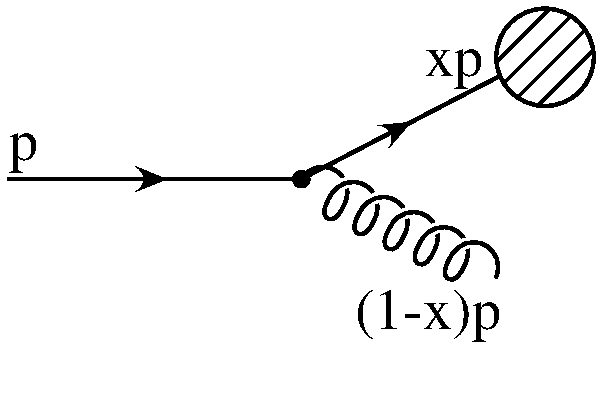
\includegraphics[width=\textwidth]{images/initial_real.pdf}
	\end{subfigure}
	\hspace{1cm}
	\begin{subfigure}[]{0.3\textwidth}
		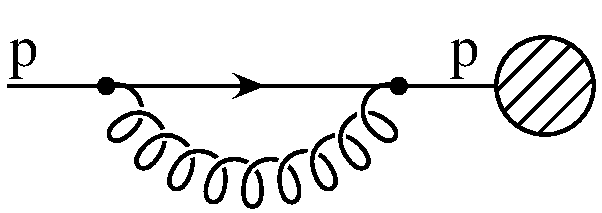
\includegraphics[width=\textwidth]{images/initial_virtual.pdf}
	\end{subfigure}
	\caption{Feynman diagrams for initial-state gluon emission.}
	\label{fig:initial_gluon}
\end{figure}
%
However, there is an important difference between real and virtual emissions in this case:
While the virtual emission does not change the momentum of the parton entering the process, the real gluon carries off parts of the parton momentum.
Thus, the total cross section consists of two different hard cross sections that do not cancel in the collinear limit.
This is a consequence of the collinear limit corresponding to long-range effects of the strong interaction, which are not calculable in perturbation theory.

In order to be able to calculate cross sections with initial-state hadrons, we can take a similar approach as for the renormalization of the coupling constant and introduce a scale variable which we call the \textit{factorization scale} $\mu_F$.
All the non-perturbative parts are cut off at $\mu_F$ and absorbed into the PDF.
There is an arbitrariness in how much of the correction terms is to be factored out.
This is defined by the \textit{factorization scheme}.
Common schemes include the DIS scheme, in which all non-leading order contributions are absorbed into the PDFs, and the $\overline{MS}$ scheme, in which only the divergent parts are absorbed.
Once the factorization scheme has been chosen, it has to be used consistently in all following cross section calculations.

As an example, let us consider the cross section for a scattering process involving two initial state hadrons $h$ and $h'$ with momenta $p$ and $p'$, which now takes the factorized form
%
\begin{equation}
	\sigma_{h,h'} = \sum_{i,j} \int \dif x \dif x' f_{i/h}(x,\mu^2) \cdot \sigma_{ij}(x p,x' p',\alpha_s(\mu^2)) \cdot f_{j/h'}(x',\mu^2) \, ,
\end{equation}
%
where we have taken $\mu_R = \mu_F= \mu$ and where the sum includes all possible initial state parton combinations.
$\sigma_{ij}$ denotes the hard parton-level cross section which can be calculated in perturbation theory.
All the non-perturbative long-distance contributions are factorized into the PDFs.
%
\section{DGLAP evolution}
Analogous to the running coupling, we can define a renormalization group equation that describes the evolution of the PDFs with the factorization scale.
It is called the Dokshitzer-Gribov-Lipatov-Altarelli-Parisi (DGLAP) equation \cite{dglap1,dglap2,dglap3} and takes the form of a matrix equation spanning all quark flavors and the gluon:
%
\begin{align}
	\dod{}{\ln{\mu_F^2}} \begin{pmatrix} q_i(x,\mu_F^2) \\ g(x,\mu_F^2) \end{pmatrix} = &\frac{\alpha_s(\mu_F^2)}{2 \pi} \sum_{q_j,\bar q_j} \int_x^1 \frac{\dif z}{z} \nonumber \\
	&\begin{pmatrix}
		P_{q_i q_j}(\frac{x}{z},\alpha_s(\mu_F^2))	&	P_{q_i g}(\frac{x}{z},\alpha_s(\mu_F^2)) \\
		P_{g q_j}(\frac{x}{z},\alpha_s(\mu_F^2))	&	P_{gg}(\frac{x}{z},\alpha_s(\mu_F^2))
	\end{pmatrix}
	\begin{pmatrix} q_j(z,\mu_F^2) \\ g(z,\mu_F^2) \end{pmatrix} \, .
	\label{eq:dglap}
\end{align}
%
The $P_{i j}(x,\alpha_s)$ are called splitting functions and they imply the probability of a parton splitting into two other partons.
They are calculable in perturbation theory and are known up to NNLO \cite{splittingkernel1,splittingkernel2}.
The DGLAP equation allows to evolve the PDFs from an initial scale $Q_0$ to another scale $Q$ without further knowledge and thus is one of the most important equations of perturbative QCD.
%
\section{Next-to-leading order calculations}
\label{sec:nlo_calculations}
\ldots(need real and virtual, both seperately divergent, need to regularize)


There are two general methods that are commonly used to take care of the infrared divergences in NLO calculations, namely the \textit{slicing method} and the \textit{subtraction method}.
The slicing method introduces a small parameter $\delta$, which slices the integration region into two pieces so that it can be computed numerically.
A residual dependency on $\delta$ remains, which should be neglectable if $\delta$ is small.
However, this has to be checked in an actual calculation.
The advantage of the subtraction method is that it does not involve any approximations.

We can demonstrate the subtraction method with a simple example, that has been adopted from \cite{mcatnlo}.
Consider the expression for the expectation value of an infrared-safe observable $O$ at NLO accuracy, consisting of a Born (B), a virtual (V) und a real (R) term:
%
\begin{equation}
	\left< O \right> = \lim_{\epsilon \rightarrow 0} \int_0^1 \dif x x^{-2 \epsilon} O(x) \left[ \left( \od{\sigma}{x} \right)_B + \left( \od{\sigma}{x} \right)_V + \left( \od{\sigma}{x} \right)_R \right] \, .
\end{equation}
%
We assume that the cross sections can be written as
%
\begin{align}
	\left( \od{\sigma}{x} \right)_B &= B \delta(x) \, , \\
	\left( \od{\sigma}{x} \right)_V &= a \left( \frac{B}{2 \epsilon} + V \right) \delta(x) \, , \\
	\left( \od{\sigma}{x} \right)_R &= a \frac{R(x)}{x} \,
\end{align}
%
where $B$ and $V$ are constant factors and $\lim_{x \rightarrow 0} R(x) = B$.
$a$ denotes the coupling constant.
Obviously, both the real and the virtual part are divergent in the limit $\epsilon \rightarrow 0$.
Using the subtraction method, we can rewrite the real contribution to obtain
%
\begin{align}
	\left< O \right>_R	&= a \lim_{\epsilon \rightarrow 0} \int_0^1 \frac{\dif x}{x^{1+2 \epsilon}} O(x) R(x) \nonumber \\
						&= a B O(0) \lim_{\epsilon \rightarrow 0} \int_0^1 \frac{\dif x}{x^{1+2 \epsilon}} + a \int_0^1 \frac{\dif x}{x} [O(x) R(x) - B O(0)] \nonumber \\
						&= -a B O(0) \lim_{\epsilon \rightarrow 0} \frac{1}{2 \epsilon} + a \int_0^1 \frac{\dif x}{x} [O(x) R(x) - B O(0)] \, .
	\label{eq:toymodel_realsub}
\end{align}
%
By explicitely writing down the virtual part,
%
\begin{equation}
	\left< o \right>_V = a \lim_{\epsilon \rightarrow 0} \int_0^1 \frac{\dif x}{x^{2 \epsilon}} O(x) \left( \frac{B}{2 \epsilon} + V \right) \delta(x) \, ,
\end{equation}
%
we see that the first term gets exactly cancelled by the first term on the right hand side of \eqref{eq:toymodel_realsub}.
Including the Born contribtion we arrive at the expression
%
\begin{equation}
	\left< O \right> = B O(0) + a \left\{ V O(0) + \int_0^1 \frac{\dif x}{x} [O(x) R(x) - B O(0)] \right\} \, ,
\end{equation}
%
which now only consists of finite terms.
The remaining integral can be evaluated using Monte Carlo methods.
The subtraction method can be generalized to arbitrary hadronic cross sections, provided that the definition of the observables allows the cancellation of the divergences.
%
\section{Parton showers}
There are phase space regions that cannot be well described by fixed order calculations in perturbation theory.
These include collinear parton splitting and soft gluon emission, which are closely related to the presence of infrared divergences.
To describe them accurately, higher order terms need to be considered.
However, the work required to derive the needed matrix elements quickly increases with each order, which is the reason why most processes have not been calculated further than NLO.
We need a different approach to deal with the problematic phase space regions.
Instead of relying on a fixed order calculation, we can consider an approximate model that includes the dominant contributions at all orders.
In this model, the collinear splitting and soft gluon emission of every parton in the initial and final state is simulated with respect to the related probabilities.
The additional partons are again able to split or radiate gluons.
By recursively applying this procedure, we obtain a cascade of parton emissions, called a \textit{parton shower}.
An example is illustrated in \cref{fig:partonshower}.
The shower ends when a certain cut-off scale is reached.
%
\begin{figure}[]
	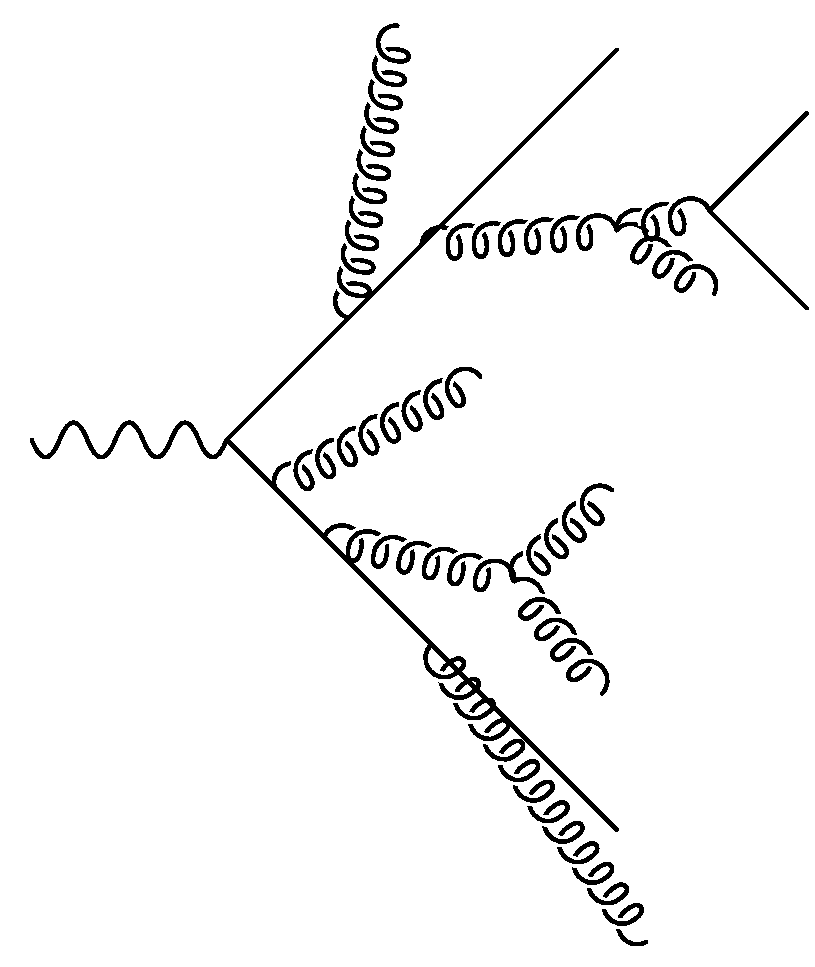
\includegraphics[width=0.5\textwidth]{images/partonshower.pdf}
	\caption{Example of a parton shower.}
	\label{fig:partonshower}
\end{figure}
%

The evolution of the splitting with the decreasing scale is given by the DGLAP equation \cref{eq:dglap}.
In this context the PDFs do not describe the momentum distributions of the partons inside of a hadron, but rather the distribution of the momentum fractions of the partons resulting from the splitting.

The computation of parton showers can be formulated in a way that is well suited for a Monte Carlo program.
We can combine the parton shower program with a hadronization model, that combines both the initial state and the final state partons into colorless hadrons, beginning at the cutoff scale of the shower. We call the result a \textit{parton shower Monte Carlo event generator}.
It is a powerful tool that is able to fully simulate QCD events in hadron collisions.

The main disadvantage of parton shower generators is that they are not guaranteed to properly describe events that include hard and large-angle emissions.
Those events are, however, correctly described by fixed order calculations.
To combine the benefits of both, algorithms have been developed that merge LO matrix elements and parton showers with different multiplicities (MEPS).
The main issue in the course of this is double counting.
An event with $n$ partons in the final state can either be the product of an $n$-parton matrix element that has been showered with only soft and collinear emissions or it could be the product of an $(n-1)$-parton matrix element for which the showering led to the emission of a hard, large-angle gluon.
Those cases have to be carefully seperated to avoid an overrepresentation of the related phase space region.
The most widely used methods to avoid double counting are CKKW matching \cite{ckkw_a,ckkw_b} and MLM matching \cite{mlm_a,mlm_b}.

Another problem of parton shower predictions is that they suffer from strong scale dependence because they are based on LO matrix elements.
Promoting parton showers to NLO accuracy is a much harder task because of divergent event weights.
Nonetheless, there are methods to circumvent this problem and the two widely used solutions are \mcatnlo{} \cite{mcatnlo} and \powheg{} \cite{powheg_a,powheg_b,powheg_c}.
As of recently, it is also possible to merge different jet multiplicities in NLO calculations matched to parton showers \cite{nlomerging1,nlomerging2,nlomerging3,nlomerging4,nlomerging5}.


% !TeX encoding=unicode
% !TeX spellcheck = de-DE

\chapter{Variation of QCD input parameters}
\label{ch:parameter_variation}
Calculations in perturbative QCD comprise uncertainties which should be determined as good as possible when they are meant to be used for predictions.
One source of uncertainty is the truncation of the perturbative series at some fixed order.
The corrections due to higher terms can only be known exactly if those terms are evaluated explicitly.
As that is no suitable approach, a good practice has evolved that consists of varying the renormalization and factorization scales in a specific range and checking how much the cross section changes by this variation.
This is based on the fact that the scale parameters are arbitrary variables, introduced in the renormalization procedure, and have no physical meaning.
Physical observables do not depend on the scale parameters and therefore in perturbative calculations a strong dependence on the scales indicates that higher order terms could give large corrections.
Additional uncertainties come from the strong coupling constant $\alpha_s$ and the choice of the PDF.
They suffer from errors in the experimental data and depend on the assumptions that are used during the fit.

For a differentiated estimate of the full uncertainty, a cross section calculation has to be repeated with different input values.
When the number of variations becomes large, it is not practical to rerun the whole event generation for each calculation as the time and resource consumption become too high.
Instead it is possible to reuse information from previously generated events and combine them with the new parameters.
In the following, two different methods are presented.
%
\section{Reweighting QCD calculations}
If we want to change the parameters in a calculation, we need to know exactly how the individual terms depend on those parameters.
Here we consider an NLO calculation using Catani-Seymour subtraction \cite{catani_seymour1997}, which is the scheme implemented in \sherpa{} and \mcgrid{}.
Other subtraction schemes can be used as well, as is demonstrated in \cite{amcfast} for the FKS scheme \cite{fks_a,fks_b}.

The total cross section can be separated into four finite terms:
%
\begin{equation}
	\sigma^\text{NLO}_{pp \rightarrow X} = \int \dif \hat \sigma^B + \int \dif \hat \sigma^V + \int \dif \hat \sigma^I + \int \dif \hat \sigma^{RS} \,
\end{equation}
%
They correspond to the Born (B), virtual (V), integrated subtraction (I) and real subtraction (RS) parts of the calculation.
We need to work out the explicit dependence on the parameters to accurately reweight them.
For the B and RS terms this is straightforward as they resemble LO calculations.
Making use of the factorization theorem we can write them in the form (cf. \cref{eq:hadron_crosssection})
%
\begin{equation}
	\sigma^{B/RS} = \sum_{i,j} \int \dif x_1 \dif x_2 \int \dif \Phi_n \left( \frac{\alpha_s(\mu_R^2)}{2 \pi} \right)^p \pdf_i(x_1,\mu_F^2) \pdf_j(x_2,\mu_F^2) \dif \hat\sigma \, ,
\end{equation}
%
where for the B term $p = p_\text{LO}$ and for the RS term $p = p_\text{LO} + 1$.
Using Monte Carlo integration, we can rewrite this as a sum over generated events:
%
\begin{equation}
  \int \dif \hat \sigma^{B/RS} = \sum_{e=1}^{N_\text{evt}} \alpha_s^p(\mu_R^2) \pdf_1(x_1,\mu_F^2) \pdf_2(x_2,\mu_F^2) w_e^{(0)} \, ,
  \label{eq:reweight_lo}
\end{equation}
%
where the weight $w_e^{(0)}$ contains the parton-level matrix element squared.

The virtual part occupies a more complicated structure because the weights explicitly depend on the renormalization scale.
It takes the form
%
\begin{equation}
	\int \dif \hat \sigma^V = \sum_{e=1}^{N_\text{evt}} \alpha_s^{p_\text{LO} + 1}(\mu_R^2) \pdf_1(x_1,\mu_F^2) \pdf_2(x_2,\mu_F^2) \left\{ w_e^{(0)} + l_R w_e^{(1)} + l_R^2 w_e^{(2)} \right\} \, ,
\end{equation}
%
with renormalization scale logarithms $l_R = \log\left(\frac{\mu_R^2}{\mu_{R,0}^2} \right)$, where $\mu_{R,0}$ is the scale at which $w_e^{(1)}$ and $w_e^{(2)}$ were originally evaluated.

In the I part, the event weights have a complex dependence on the PDF.
The full structure can be written as
%
\begin{align}
	\int \dif \hat \sigma^I = \sum_{e=1}^{N_\text{evt}} &\alpha_s^{p_\text{LO} + 1}(\mu_R^2) \left\{ \vphantom{\left( \sum_{k=1}^4 \right)} f_1(i,x_1,\mu_F^2) w_e^{(0)} f_2(j,x_2,\mu_F^2) \right. \nonumber \\
								&+ \left( \sum_{k=1}^4 f_1^{(k)}(i,x_1,x'_1,\mu_F^2) w_{e,k}^{(3)} \right) f_2(j,x_2,\mu_F^2) \nonumber \\
								&\left. + f_1(j,x_1,\mu_F^2) \left( \sum_{k=1}^4 w_{e,k}^{(4)} f_2^{(k)}(j,x_2,x'_2,\mu_F^2) \right) \right\} \, ,
\end{align}
%
where the $x$ and $x'$ are the Björken-$x$ before and after initial state branching.
Moreover, $i$ and $j$ denote the parton flavors before the branching and the $f^{(k)}$ provide the correct form of the PDF depending on the type of branching.
They are given explicitly in \cite{mcgrid2013}.

We can dispose of the weights $w^{(1)}$ and $w^{(2)}$ by choosing a central scale.
If we furthermore project the contributions from $w^{(3)}$ and $w^{(4)}$ onto separate events, we can write the total NLO cross section in the compact form
%
\begin{equation}
  \sigma^\text{NLO}_{pp \rightarrow X} = \sum_{e=1}^{N_\text{evt}} \alpha_s^{p_e}(\mu_R^2) \pdf_1(x_1,\mu_F^2) \pdf_2(x_2,\mu_F^2) w_e \, ,
  \label{eq:reweight_nlo}
\end{equation}
%

Provided that all event weights have been stored, it is now possible to change the values of $\alpha_s$, $\mu_R$ and $\mu_F$ or use a different PDF \textit{a posteriori}.
%
\section{Interpolation grids}
Despite the advantage towards regenerating all events for the variation of a single parameter, the reweighting approach is still not a satisfying solution for many use cases.
The whole event record has to be stored, which can easily reach many gigabytes or even terabytes in high statistics computations.
The storing and reprocessing of the events may be a challenge by itself and is not convenient if more than a few parameter variations have to be performed.
One therefore wishes to somehow decrease the resource requirements without losing a significant amount of accuracy.
In the ideal case, it should be mostly independent of the statistics.
A possible solution is the use of interpolating grids to represent the PDFs and event weights.
Then only a uniquely defined number of values has to be saved, while values in-between the grid points are generated by interpolating functions.
Such a method has been implemented by the \appl{} \cite{applgrid2010} and \fnlo{} \cite{fastnlo2006,fastnlo2011} projects.

The PDF $\pdf(x,Q^2)$ depends on the momentum fraction $x$ and the scale $Q^2$.
It can be approximated as a sum over discrete grid points using interpolation functions $I$ of order $N$:
%
\begin{equation}
	\pdf(x,Q^2) = \sum_{i=0}^{N_x} \sum_{j=0}^{N_Q} \pdf(x_i,Q_j^2) I_i^{(N_x)}(x_1) I_j^{(N_Q)}(Q^2) \, .
\end{equation}
%
Consequently, we can write \cref{eq:reweight_nlo} as
%
\begin{alignat}{3}
  \sigma^\text{NLO}_{pp \rightarrow X}	&= \sum_{e=1}^{N_\text{evt}} \sum_{i,j=0}^{N_x} \sum_{k=0}^{N_Q} &&\alpha_s^{p_e}(Q_k^2) \pdf_1(x_i,Q_k^2) \pdf_2(x_j,Q_k^2) w_e \nonumber \\
  										&	&&\cdot I_i^{(N_x)}(x_1) I_j^{(N_x)}(x_2) I_k^{(N_Q)}(Q^2) \nonumber \\
  										&= \mathrlap{\sum_p \sum_{i,j=0}^{N_x} \sum_{k=0}^{N_Q} \alpha_s^p(Q_k^2) \pdf_1(x_i,Q_k^2) \pdf_2(x_j,Q_k^2) W_{i,j,k}^{(p)} \, ,}
\end{alignat}
%
where $p$ is the perturbative order and the interpolated weights $W_{i,j,k}^{(p)}$ are processed as a sum over the events:
\begin{equation}
	W_{i,j,k}^{(p)} = \sum_{e=1}^{N_\text{evt}} \delta_{p,p_e} w_e I_i^{(N_x)}(x_1) I_j^{(N_x)}(x_2) I_k^{(N_Q)}(Q^2) \, .
\end{equation}
%
Now the sum over the events has been completely absorbed into the definition of the interpolated weights.
These can be calculated in a single run of the event generator and be stored efficiently.
The calculation of the cross section has become a simple sum over the grid points and thus is much faster for a large number of events.
The approach can easily be extended to histogrammed data like differential cross sections by defining the observable bins and computing one weight $W_{i,j,k}^{(p),(s),(b)}$ for each bin $b$.
However, unlike the full event record, the weight grid is restricted to the observable it was constructed for and cannot be used to calculate any other values.

While the variation of the PDF and $\alpha_s$ is still straightforward, scale variation is slightly more complicated because the weights themselves depend on the scale choices.
Nevertheless, it is possible to vary the scales without too much effort, using DGLAP evolution.
The precise procedure is explained in \cite{applgrid2010}.

% !TeX encoding=unicode
% !TeX spellcheck = de-DE

\chapter{The considered process: Higgs production through gluon fusion}
\label{ch:gfusion}
%
\section{Gluon fusion at the LHC}
The Englert-Brout-Higgs-Guralnik-Hagen-Kibble mechanism (commonly Higgs mechanism) explains the non-zero masses of the gauge bosons in the standard model.
It has been developed in the 1960s with important contributions coming from several people \cite{higgs1964a,higgs1964b,englert1964,guralnik1964,nambu1960,anderson1963}.
It invokes the process of spontaneous symmetry breaking and evades the Goldstone theorem.
In the development of the standard model, the Higgs mechanism played a key role and ever since the discovery of the Higgs boson in 2012 by ATLAS \cite{higgsdiscovery_atlas2012} and CMS \cite{higgsdiscovery_cms2012} at the LHC it has received wide approval.

In this thesis, the considered process is the production of a Higgs boson through gluon fusion.
Although there are other possible production mechanisms in the Standard Model, this is the main process at the LHC, with an expected cross section of $\approx \SI{50}{\pico\barn}$ at a center-of-mass energy of $\sqrt{s} = \SI{14}{\tera\electronvolt}$ and a Higgs mass of $\SI{125}{\giga\electronvolt}$ \cite{higgshandbook1}.
It proceeds through a triangular loop of heavy quarks (mainly top quarks as the Higgs coupling scales with the quark mass) as is shown in \figref{fig:gluonfusion}.
%
\begin{figure}[]
	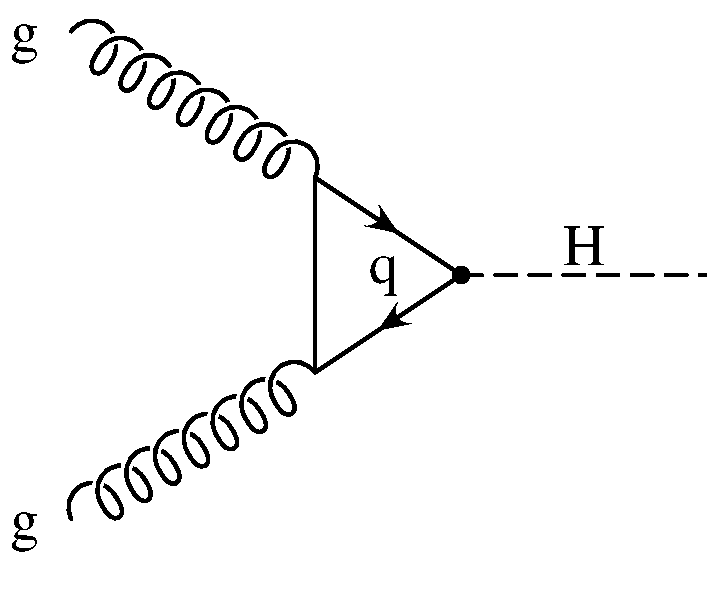
\includegraphics[width=0.5\textwidth]{images/gluonfusion.pdf}
	\caption{Higgs production through gluon fusion.}
	\label{fig:gluonfusion}
\end{figure}
%

In the narrow-width approximation, the leading order cross section is given by \cite{gluonfusioncrosssection}
%
\begin{equation}
	\sigma_\text{LO}(pp \rightarrow H) = \sigma_0^H \tau_H \od{\lumi^{gg}}{\tau_H} \, ,
\end{equation}
%
where $\tau_H = M_H^2/s$ is the Drell-Yan variable and $\dif \lumi^{gg} / \dif \tau_H$ is the gluon luminosity.
The partonic cross section $\sigma_0^H$ can be written as
\begin{equation}
	\sigma_0^H = \frac{G_F \alpha_s^2(\mu_R^2)}{288 \sqrt{2} \pi} \abs{ \sum_q \frac{3}{2 \tau_q} \left[ 1 + \left( 1 - \frac{1}{\tau_q} \right) f(\tau_q) \right] }^2  \, ,
\end{equation}
%
with the form factor
%
\begin{equation}
	f(\tau_q) = 
	\begin{cases}
		\arcsin^2 \left( \sqrt{\tau_q} \right) ,																& \tau_q < 1, \\
		- \frac{1}{4} \left[ \ln \frac{1 + \sqrt{1-\tau_q^{-1}}}{1 - \sqrt{1-\tau_q^{-1}}} -i \pi \right]^2 ,	& \tau_q > 1,
	\end{cases}
\end{equation}
%
where $G_F$ denotes the Fermi coupling constant and $\tau_q = m_H^2/4m_q^2$.
The gluon luminosity takes the form
%
\begin{equation}
	\od{\lumi^{gg}}{\tau_H} = \int_0^1 \dif x_1 \dif x_2 \gluonpdf(x_1,\mu_F^2) \gluonpdf(x_2,\mu_F^2) \delta(x_1 x_2 - \tau_q) \,
\end{equation}
%
with $\gluonpdf(x,\mu_F^2)$ denoting the gluon PDF.

The QCD corrections are composed of virtual corrections to the vertices and propagators, real gluon radiation in the initial state and the contributions of the subprocesses $gq \rightarrow Hq$ and $q \bar q \rightarrow Hg$.
Exemplary diagrams for the corrections are shown in \figref{fig:ggh_corrections}.
The full NLO cross section has been calculated in \cite{gfusionnlo1,gfusionnlo2,gfusionnlo3}.
They increase the cross section by a factor of \num{1.5} to \num{1.7}.
%
\begin{figure}
\centering
\begin{subfigure}[]{0.3\textwidth}
	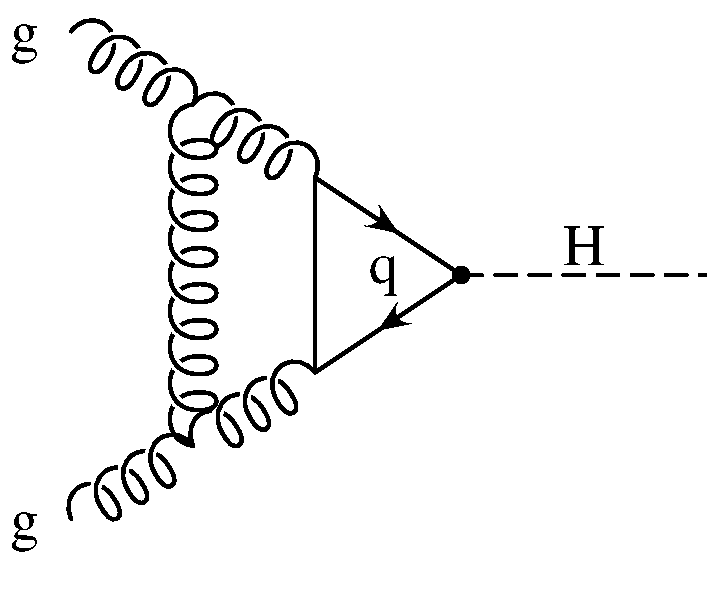
\includegraphics[width=\textwidth]{images/gluonfusion_virtual1.pdf}
	\caption{}
\end{subfigure}
~
\begin{subfigure}[]{0.3\textwidth}
	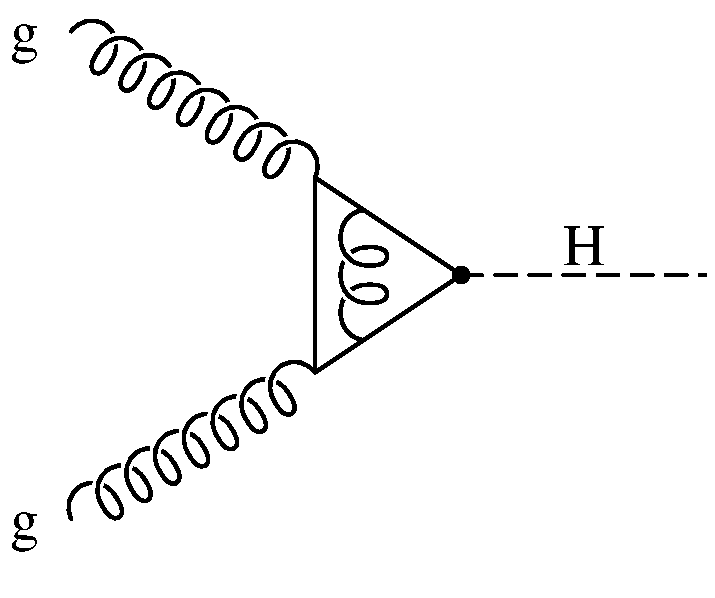
\includegraphics[width=\textwidth]{images/gluonfusion_virtual2.pdf}
	\caption{}
\end{subfigure}
~
\begin{subfigure}[]{0.3\textwidth}
	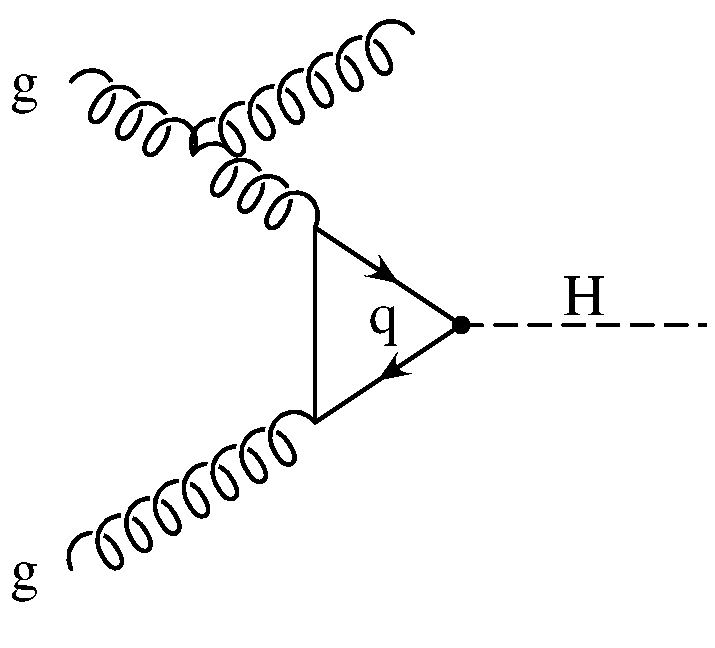
\includegraphics[width=\textwidth]{images/gluonfusion_real1.pdf}
	\caption{}
\end{subfigure}

\begin{subfigure}[]{0.3\textwidth}
	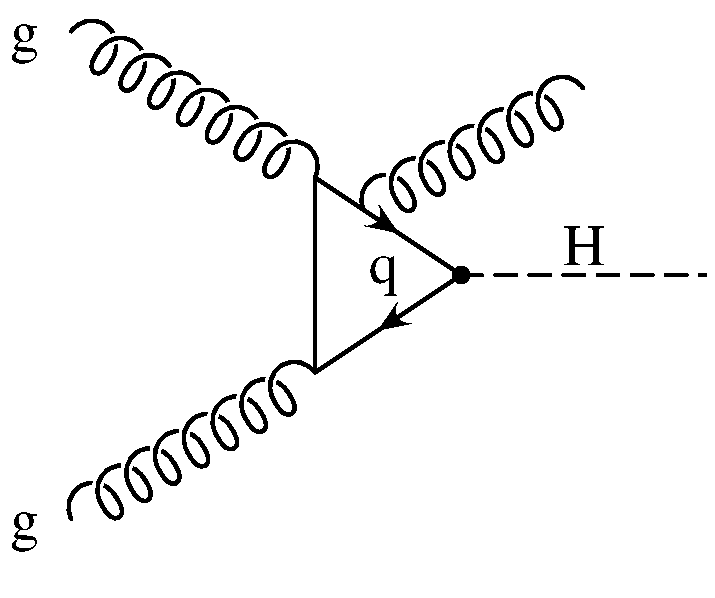
\includegraphics[width=\textwidth]{images/gluonfusion_real2.pdf}
	\caption{}
\end{subfigure}
~
\begin{subfigure}[]{0.3\textwidth}
	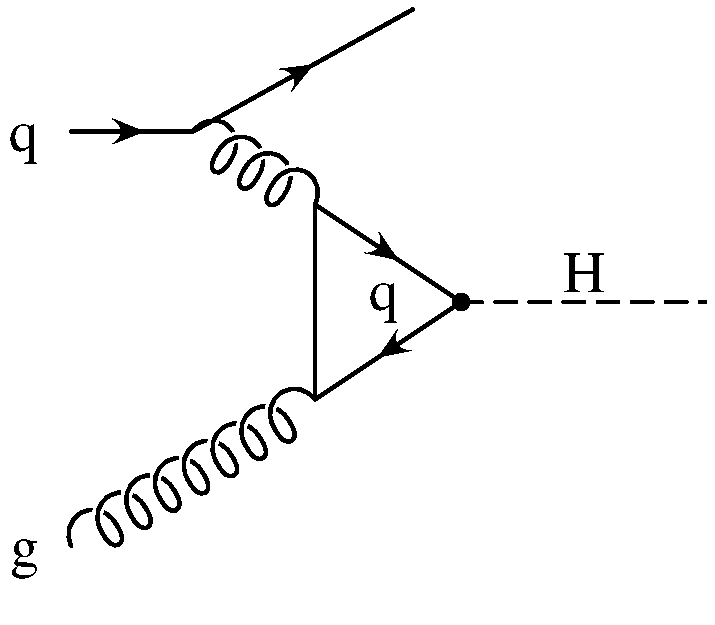
\includegraphics[width=\textwidth]{images/gq_hq.pdf}
	\caption{}
\end{subfigure}
~
\begin{subfigure}[]{0.3\textwidth}
	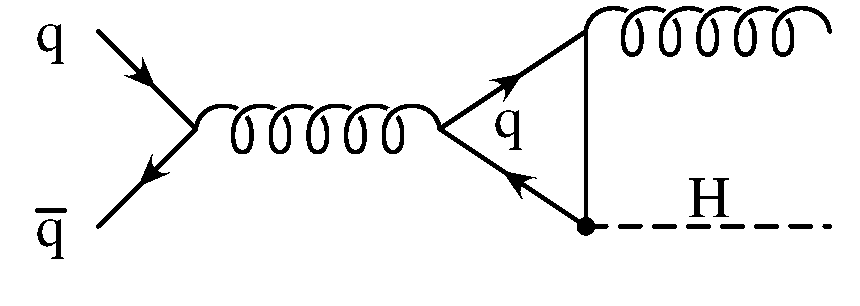
\includegraphics[width=\textwidth]{images/qq_hg.pdf}
	\caption{}
\end{subfigure}
\caption{Example diagrams illustrating the QCD corrections to the process $pp \rightarrow H$:
		(a), (b) virtual corrections; (c), (d) real emission of a gluon; (e) $gq \rightarrow Hq$; (f) $q \bar q \rightarrow Hg$.}
\label{fig:ggh_corrections}
\end{figure}
%

In the limit where the top quark has infinite mass, $m_t \rightarrow \infty$, the form factor takes the value $\frac{4}{3}$.
This allows for an analytical expression of the corrections \cite{gfusionnlo2}.
It can be considered as an extension of the Standard Model, where the Higgs boson couples directly to gluons, known as effective Higgs coupling (cf. \cref{fig:heft}).
The effective Lagrangian for Higgs gluon interaction can be written as \cite{gfusionnnlo2}
%
\begin{equation}
	\Lagr_\text{eff}^{ggH} = - \frac{1}{4v} C_1 G_{\mu \nu}^a {G^a}^{\mu \nu} H \, ,
\end{equation}
%
where $v$ is the Higgs vacuum expectation value, $G^a_{\mu \nu}$ is the gluon field strength tensor and $H$ is the Higgs field.
The coefficient $C_1$, in the \msbar{} scheme, is given by
%
\begin{align}
	C_1 = \frac{-1}{3 \pi} &\left\{1 + \frac{11 \alpha_s}{4 \pi} + \left( \frac{\alpha_s}{\pi} \right)^2 \left[ \frac{2777}{288} + \frac{19}{16} \log\left( \frac{\mu^2}{m_t^2} \right)
	\vphantom{n_f \left( -\frac{67}{96} + \frac{1}{3} \log\left( \frac{\mu^2}{m_t^2} \right) \right)} \right. \right. \nonumber \\
	%	
		&\qquad \left. \left. \vphantom{\frac{2777}{288} + \frac{19}{16} \log\left( \frac{\mu^2}{m_t^2} \right)}
		+ n_f \left( -\frac{67}{96} + \frac{1}{3} \log\left( \frac{\mu^2}{m_t^2} \right) \right) \right] + \order{\alpha_s^3} \right\} \, ,
\end{align}
%
where the number of active flavors should be set to $n_f = 5$.
According to \cite{gfusionnnlo2}, at LO this approximation is accurate within \SI{5}{\percent} for $m_H \approx \SI{150}{\giga\electronvolt}$ (which is close to the measured value $m_H \approx \SI{126}{\giga\electronvolt}$) and improves at NLO.
All calculations in this thesis are based on effective Higgs coupling.
%
\begin{figure}[]
	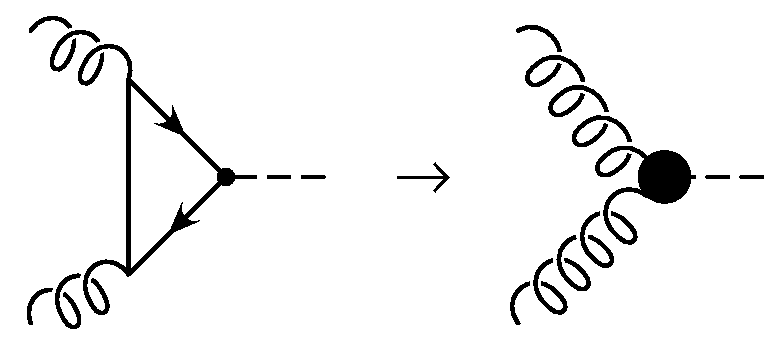
\includegraphics[width=0.5\textwidth]{images/heft.pdf}
	\caption{Effective Higgs coupling.}
	\label{fig:heft}
\end{figure}
%

Besides the basic process, the fully differential NLO cross sections are available for $H + 1$ jet \cite{gghj_nlo_fullydiff_1,gghj_nlo_fullydiff_2}, $H + 2$ jets \cite{gghjj_nlo_fullydiff_1,gghjj_nlo_fullydiff_2} and $H + 3$ jets \cite{gghjjj_nlo_fullydiff}.
A fully differential NNLO calculation exists for $H + 0$ jets production \cite{ggh_nnlo_fullydiff_1,ggh_nnlo_fullydiff_2} and substantial progress has been achieved towards an NNLO calculation of the $H + 1$ jets cross section \cite{gghj_nnlo_progress}.
%
\section{Leptonic Higgs decay}
In an experiment, one would never observe the Higgs boson directly but rather reconstruct it from the measured properties of its decay products.
We want to approximate this situation by simulating the Higgs boson decay.
There are several possible decay channels.
One has to keep in mind that the Higgs coupling is proportional to the particle masses, so that it will decay into the heaviest possible particles.
Assuming a Higgs mass of $m_H = \SI{126}{\giga\electronvolt}$, the most relevant decay products are $q \bar q$ (where q denotes a bottom or charm quark), $WW$, $ZZ$, $Z \gamma$, $\gamma \gamma$, $gg$ and $\tau^+ \tau^-$ \cite{higgshandbook2}.
The decay into photons or gluons is only possible through intermediate loops.
The studies leading to the discovery of the Higgs boson at the LHC relied primarily on the decay modes $H \rightarrow \gamma \gamma$, $H \rightarrow ZZ$ and $H \rightarrow WW$.

For the purpose of this thesis, we will consider the decay $H \rightarrow \tau^+ \tau^-$, which has a branching ratio of approximately \SI{6}{\percent} \cite{higgshandbook3}.
The Feynman diagram is shown in \cref{fig:h_tautau}.
It would be possible to simulate the other decay channels as well, however, this would only complicate the analysis unnecessarily.
The leptonic decay is the easiest one and closely resembles the Drell-Yan process.
There have been searches for $H \rightarrow \tau \tau$ events in the LHC data and both ATLAS \cite{htau_atlas} and CMS \cite{htau_cms} have published evidence for this type of decay.
It also allows for the observation of additional jets that are produced in the initial state and are separated from the Higgs decay products.
We will not consider the further decay of the tau leptons, which would naturally occur in the experiment.
%
\begin{figure}[]
	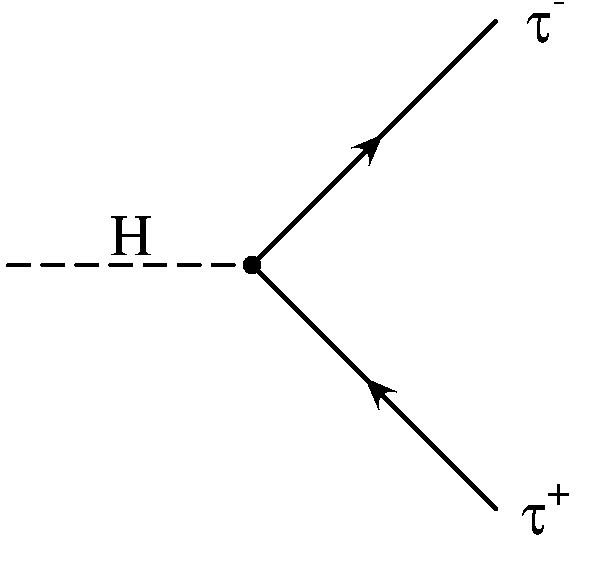
\includegraphics[width=0.5\textwidth]{images/h_tautau.pdf}
	\caption{Higgs decay into two $\tau$ leptons.}
	\label{fig:h_tautau}
\end{figure}
%
\section{The transverse momentum of the Higgs boson}
\ldots

The transverse momentum distribution of the Higgs boson is one of the most interesting observables in Higgs production.
It provides a powerful test of the standard model once the statistics of the experimental results become suitable.
In the following, we will briefly study the distribution in the gluon fusion process, where the Higgs boson is produced along with a different number of jets.
In particular, we will take a look at how the quality of the prediction is influenced by parton showers.

\ldots

Four seperate runs have been performed: One run each for zero, one and two jets at fixed order NLO and one \mcatnlo{} run merging up to two jets in the core process.
The \rivet{} analysis system has been used to extract the transverse momentum of the Higgs boson from the events.
In the multijet merged run, the cases of at least zero, one or two jets have been distinguished and sorted into different histograms.
Thus, we obtain inclusive observables that are comparable to the fixed order results.
\sherpa{} has been used for all calculations and the \mcfm{} library \cite{mcfm_hjj} has been interfaced for the 2-jet process.
For the fixed order calculations, both the renormalization and the factorization scale have been set to the transverse mass of the Higgs boson.
Final state jets have been extracted by the \fastjet{} library \cite{fastjet_manual} using the anti-$k_t$ algorithm \cite{anti_kt} with a radius parameter $R=0.4$ and a $p_\perp$-cut of $p_\perp > \SI{20}{\giga\electronvolt}$.
All the resulting histograms have been normalized to \num{1}, so that the comparison is not affected by differences in the scale definitions between the fixed order and the merged runs.
As we want to do a qualitative study rather than a quantitative one, this is no big restriction.
For the same reason no uncertainties are shown in the plots.
More detailed studies can be found in the relevant literature, cf. for example \cite{symmetrybreaking1,symmetrybreaking2} or \cite{higgshandbook1,higgshandbook2,higgshandbook3}.

\Cref{fig:h_hpt_nominal} compares the fixed order NLO and the merged \mcatnlo{} results in the case of no jets.
At NLO the tranverse momentum of the Higgs boson arises solely from real gluon emissions as the LO process does not have any tranverse parts.
The splitting leading to the real emissions is divergent in the soft and collinear limits which correspond to low transverse momenta.
Therefore, in \cref{fig:h_hpt_nominal}, we see that the cross section diverges towards low $p_\perp$.
The multijet result behaves completely different in the low $p_\perp$ region and shows no divergence.
In this case, the cross section is dominated by parton showers which include higher orders and are not divergent.
Compared to the fixed order calculation, the cross section is much smaller in the low $p_\perp$ region.
As opposed to this, the cross section is amplified for $p_\perp \gtrsim \SI{20}{\giga\electronvolt}$.
The influence of the parton shower is negligible in this region.
Instead the additional contributions come from the higher jet multiplicities that have been merged into the calculation.
At high $p_\perp$, both results approach each other.

The results containing one or more jets are compared in \cref{fig:hj_hpt_nominal}.
Due to the jet cut, Higgs $p_\perp$ below \SI{20}{\giga\electronvolt} are very unlikely and present no meaningful observable, so we do not consider that case.
At $p_\perp = \SI{20}{\giga\electronvolt}$, when the Higgs boson recoils against the jet, the cross section diverges at NLO.
Similar to the previous situation, the parton shower fixes the divergence and produces a smooth distribution.
At high $p_\perp$ the merged run gives a higher cross section, this time the additional contributions stem from the 2-jet process.

With two additional jets, the fixed order and the showered result become very similar, cf. \cref{fig:hjj_hpt_nominal}.
The core process now is the same in both cases.
Higher multiplicities in the \mcatnlo{} result are generated only by the parton shower.
The influence of the shower, though, is negligible.
%
\begin{figure}
	\centering
	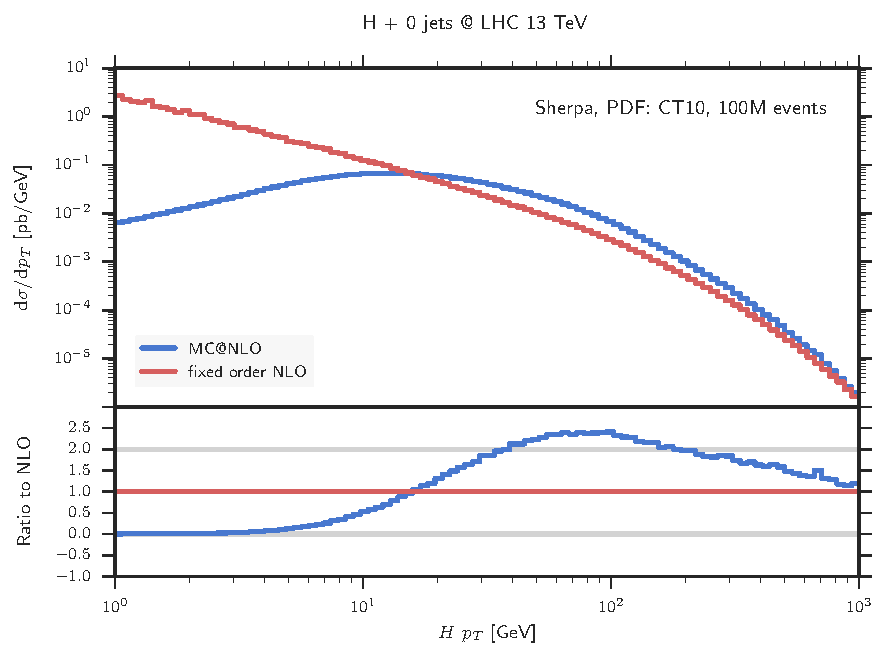
\includegraphics[width=0.8\textwidth]{images/h_hpt_nominal.pdf}
	\caption{H pT 0j}
	\label{fig:h_hpt_nominal}
\end{figure}
%
\begin{figure}
	\centering
	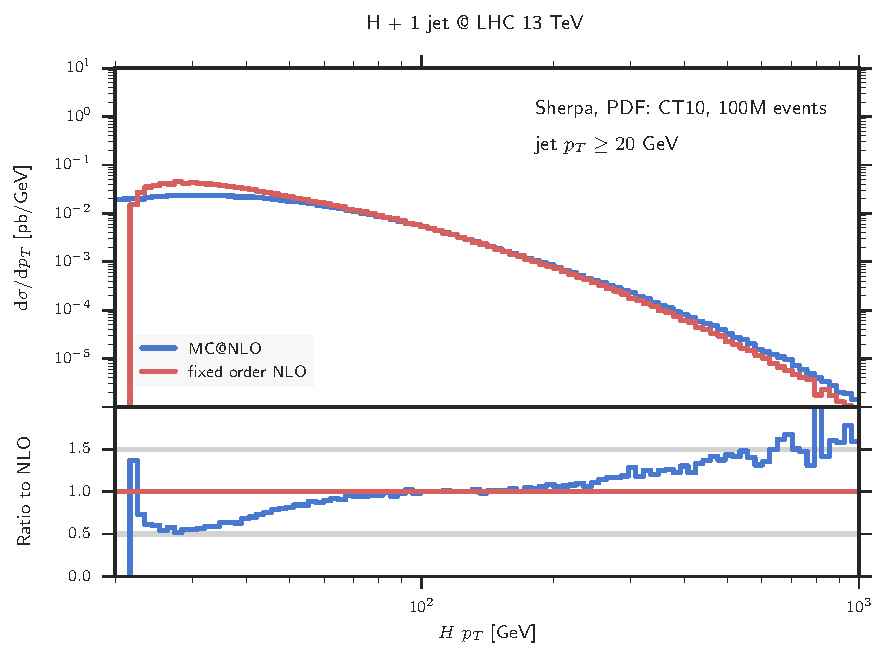
\includegraphics[width=0.8\textwidth]{images/hj_hpt_nominal.pdf}
	\caption{H pT 1j}
	\label{fig:hj_hpt_nominal}
\end{figure}
%
\begin{figure}
	\centering
	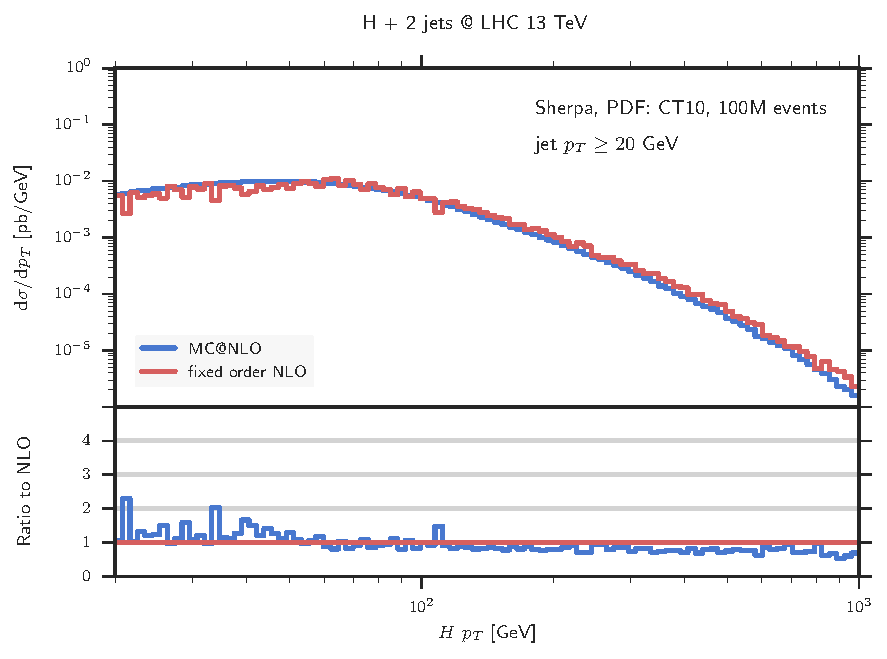
\includegraphics[width=0.8\textwidth]{images/hjj_hpt_nominal.pdf}
	\caption{H pT 2j}
	\label{fig:hjj_hpt_nominal}
\end{figure}
%

% !TeX encoding=unicode
% !TeX spellcheck = de-DE

\chapter{Validation of the interpolation method}
\label{ch:validation}
%
In the following, the interpolation method used by \mcgrid{} is validated for the processes $pp \rightarrow H + (0,1,2)$ jets at the \SI{13}{\tera\electronvolt} LHC, computed at NLO.
Thereto, reference distributions for different observables are generated using the \sherpa{} event generator and compared to the distributions obtained by convoluting a grid with the respective PDF.
Additionally, the results from \appl{} and \fnlo{} are compared to each other.
All grids are filled using the central value of the CT10 PDF set \cite{ct10}.
The examined observables are the transverse momenta $p_\perp$ of the Higgs boson and the $\tau$ leptons, respectively, the rapidity $y$ of the Higgs boson and the pseudorapidity $\eta$ of the $\tau$ leptons.
The projection of the observables into histogram bins is accomplished by the \rivet{} analysis system.
Final state jets are extracted by the \fastjet{} library \cite{fastjet_manual} using the anti-$k_t$ algorithm \cite{anti_kt} with a radius parameter $R=0.4$ and a $p_\perp$-cut of $p_\perp > \SI{20}{\giga\electronvolt}$.

The first validity test will check whether the grids are able to reproduce the distributions when they are filled with the same events as the reference histograms, i.e.\ when no parameter variation is performed.
This will also determine the interpolation accuracy.
Subsequently, the cases where the scale factors and/or PDFs of the grids are changed \textit{a posteriori} will be compared to reference distributions where these parameters have been set explicitly.
%
\section{The distribution of parton momenta}
\label{sec:xtransform}
\appl{} and \fnlo{} do not use the momentum fraction $x$ and the factorization scale $Q^2$ directly in their grids.
Instead, they provide transformations that are supposed to achieve better coverage of the values.
In the following, we will concentrate on the $x$ distribution, which is more crucial to the number of grid points needed.
The functions provided by \appl{} are:
%
\begin{align}
	f_0(x)	&= \log(\frac{1}{x} -1) \\
	f_1(x)	&= -\log(x) \\
	f_2(x)	&= \sqrt{-\log(x)} \\
	f_3(x)	&= -\log(x) + 5 \cdot (1-x) \, .
\end{align}
%
\fnlo{} only provides the functions $f_1(x)$ and $f_2(x)$.
To be used in a grid, the functions are divided into equal-sized bins.
In order to avoid empty bins, the limit values are determined in a seperate \enquote{phasespace run} before the actual fill run.

The functions (normalized to the domain $[0,1]$ for comparability) are shown in \figref{fig:xtransform}.%
%
\begin{figure}[]
	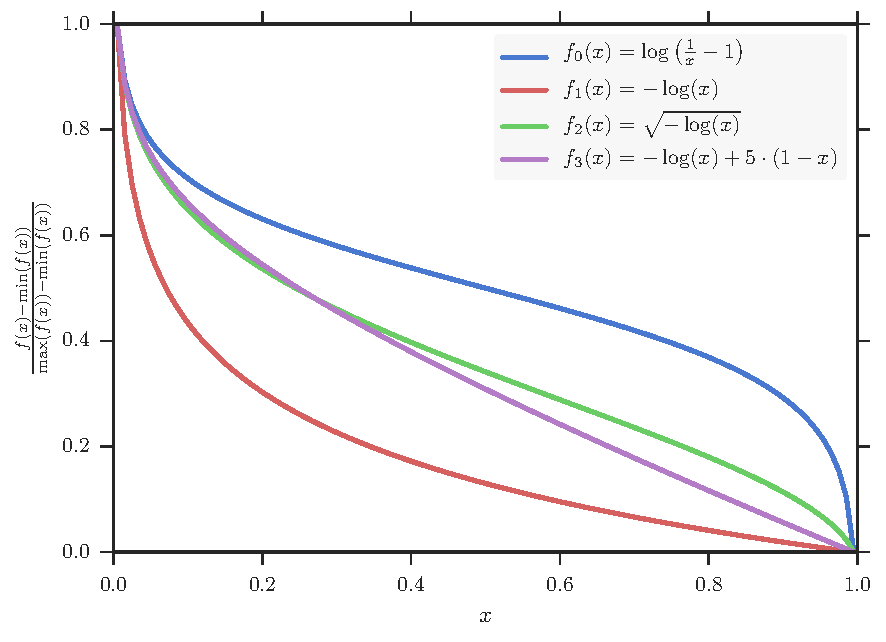
\includegraphics[width=0.7\textwidth]{images/xtransform.pdf}
	\caption{The transformations applied to the $x$ distribution, normalized to the range $[0,1]$.}
	\label{fig:xtransform}
\end{figure}
%
All transformations increase the point density in the low $x$ region, where most events should fall into.
Compared against $f_1$, the other functions also accomplish a higher point density in the high $x$ region.
Some observables in specific processes might benefit from this.

We can look at the actual $x$ distribution in the process considered in this thesis.
In \figref{fig:x_compare} it is plotted for one of the gluons involved in the process $gg \rightarrow H + j$ at leading order for a center-of-mass energy of $\sqrt{s} = \SI{13}{\tera\electronvolt}$.
For comparison, the respective distribution for the functions $f_0$ to $f_3$ is also shown.
In the bare distribution, the number of events per bin increases rapidly towards low $x$.
It is obvious that the reproduction of the low $x$ region is poor for this linear binning.
We expect that for some $x>0$ the number of events approaches zero, because there has to be at least enough momentum transfer to produce the Higgs boson and the jet.
To see this with linear binning, one would need a huge amount of bins.
In contrast, the transformations are able to project the low $x$ peak to a higher number of bins than the naive linear binning.
Additionally, they all approach zero for a finite value (note that high values of $f(x)$ correspond to low values of $x$).
Due to the normalization, this happens at $1$.
For all transformed distributions, it should be possible to interpolate them with a reasonable number of sampling points.
The function $f_1(x)$ looks most promising, as it allocates many bins for the peak region, which should be the most relevant for this process.

%
\begin{figure}[]
	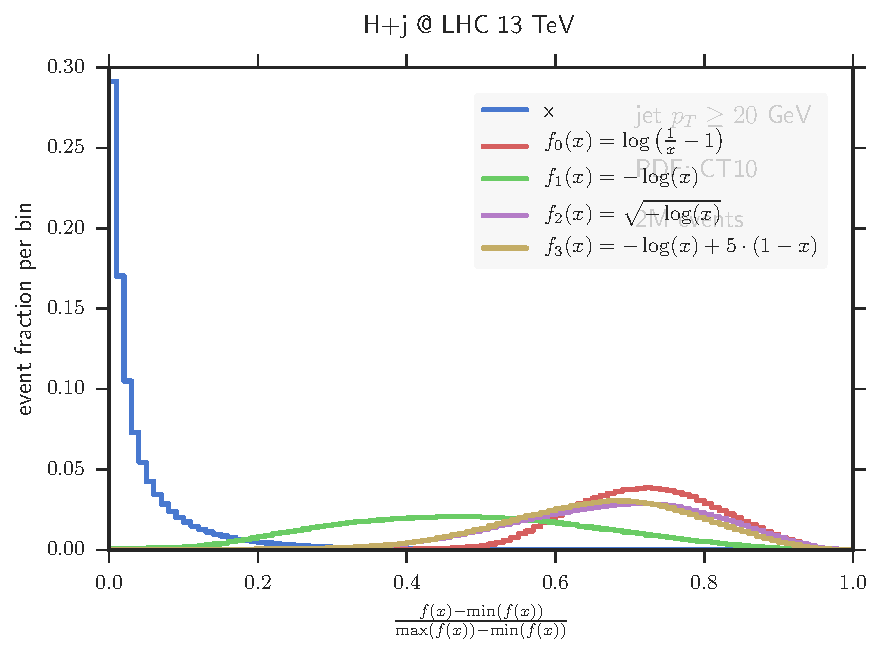
\includegraphics[width=0.7\textwidth]{images/x_compare.pdf}
	\caption{The event fraction per bin for the different transformations.}
	\label{fig:x_compare}
\end{figure}
%

If we want to be more specific, we can extract the dependence of the observables on $x$ and $f(x)$, respectively, from the generated events.
This is shown in \figref{fig:hpt_compare} for the transverse momentum $p_\perp$ and in \figref{fig:hy_compare} for the rapidity $y$ of the Higgs boson.
We see that the rapidity heavily depends on low $x$ values.
One half of the contributions comes from values $x \leq \num{0.03}$.
Values above \num{0.3} are in practice negligible.
The transformations reveal a substructure of the peak that is impossible to see with the linear binning.
Compared to the rapidity, the transverse momentum has a higher percentage of high $x$ values.
Nevertheless, it is still dominated by the low $x$ region.

For both observables all considered functions are a reasonable choice.
Especially for the rapidity, the function $f_1(x)$ seems to be best suited.
Hence, it will be the transformation used in all following grid calculations.
%
\begin{figure}[]
	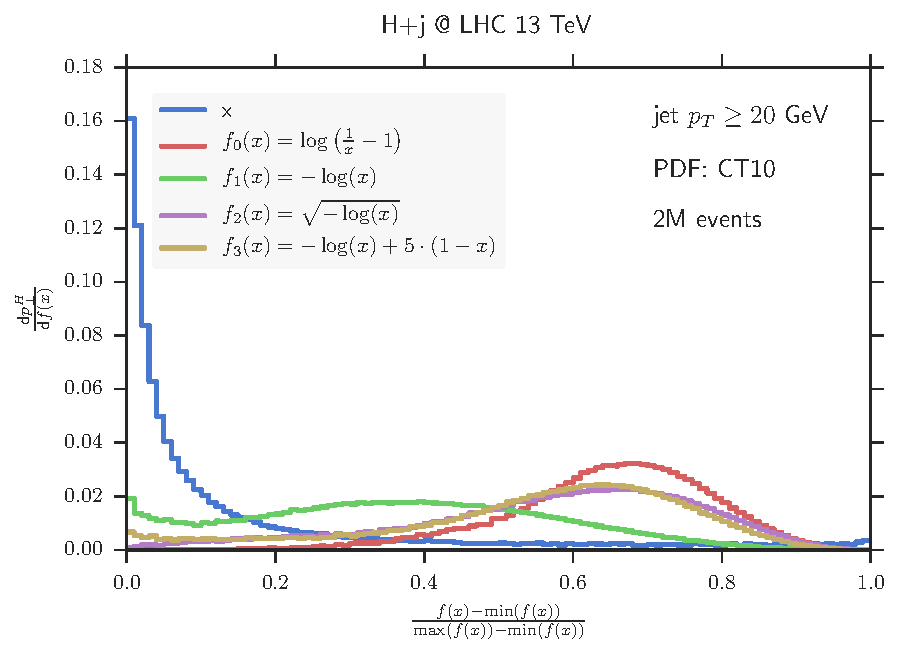
\includegraphics[width=0.7\textwidth]{images/hpt_compare.pdf}
	\caption{The transverse momentum $p_\perp$ of the Higgs boson differential in f(x).
				The ordinate shows the fraction per bin.}
	\label{fig:hpt_compare}
\end{figure}
%
\begin{figure}[]
	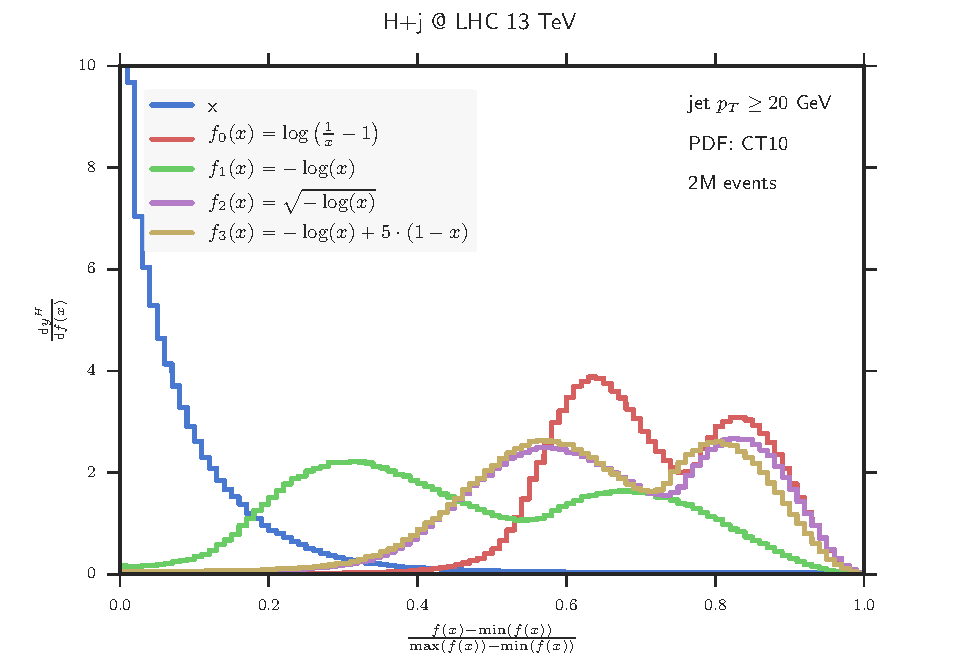
\includegraphics[width=0.7\textwidth]{images/hy_compare.pdf}
	\caption{The rapidity $y$ of the Higgs boson differential in f(x).
				The ordinate shows the fraction per bin.}
	\label{fig:hy_compare}
\end{figure}
%
\section{Interpolation accuracy}
In this section we will prove, that the grids are able to reproduce the reference distributions up to the available interpolation accuracy.
For each observable, one high precision grid and one lower precision grid is used.
In the 0- and 1-jet cases, the high precision grid has \num{50} bins in $x$ and the lower precision grid has \num{30} bins in $x$.
In the 2-jet case, the high precision grid has \num{70} bins and the lower precision one has \num{50} bins.
This is because with higher jet multiplicity, the influence of high $x$ values increases while in all cases the same transformation is used to smooth the distribution.
As we have seen in \cref{sec:xtransform}, this transformation favors low values of $x$, so a relatively high number of grid points is needed to accurately represent the high $x$ region.
For all the following calculations, the scale parameters have been fixed to the mass of the Higgs boson.
Therefore, $Q^2$ does not change and only one bin is used.
To achieve better comparability, \appl{} is configured to use fourth order interpolation, which is the same as is hardcoded into the \fnlo{} library.
A sample of \num{10} million events is used to fill the grids.

\Cref{fig:hnlo_validation} shows the ratio of the results obtained by convoluting the grids with the CT10 PDF to the reference distributions for the 0-jet process.
Using the high precision grid, all errors are below \SI{0.1}{\percent}.
\appl{} and \fnlo{} show roughly the same accuracy.
The effect of using a smaller grid is considerably bigger for the $p_\perp$ distributions than for the rapidity distributions.
This can be understood by looking back at \cref{fig:hpt_compare,fig:hy_compare} in \cref{sec:xtransform}.
There we saw, that high values of $x$ are completely negligible for the rapidity distribution and that it can be interpolated very well by using a logarithmic transformation.
The $p_\perp$ distribution is still dominated by small values of $x$, but compared to the rapidity large $x$-values have a bigger influence.
Thereby, the interpolation is not as optimal.
Here, the smaller grid also has a more severe impact on the \appl{} result than on the \fnlo{} one.

With one jet (\cref{fig:hjnlo_validation}), the errors in the reproduction of the $p_\perp$ become notably larger.
Even with the high precision grid, \fnlo{} produces errors for individual bins of the $p_\perp$ distributions, that are large compared to the other bins.
The errors of the largest outliers are about \SI{2}{\percent}.
In comparison, the errors produced by \appl{} with the high precision grid are of the order of \SI{0.01}{\percent}.
The main difference between the two packages that remains in the used configuration is the interpolation function.
Both use a kind of Lagrangian polynomials, but the implementations differ.
It might be possible, that the function used by \appl{} is more appropriate in this case.
Nonetheless, the reproduction of the rapidity distributions is still very good with all grids.
This is because the rapidity is not much influenced by additional jets.

The case of two jets is shown in \cref{fig:hjjnlo_validation}.
Here the grids with \num{50} bins produce relatively large errors.
With the high precision grid, however, \appl{} still allows a very good reproduction.
\fnlo{}, by contrast, features large outliers with errors of several percent.
This can be attributed to the statistics.
\Cref{fig:hpt_100m} proves that the reproduction is much better with a 100 million event sample, albeit still being worse than with \appl{}.
The problem with the $H + 2j$ process is that the event generator produces many negative weights, so that high statistics is needed to obtain a smooth distribution.
For some reason, this affects \fnlo{} more than \appl{}.
%
\begin{sidewaysfigure}
\centering
\begin{subfigure}[]{0.49\textwidth}
	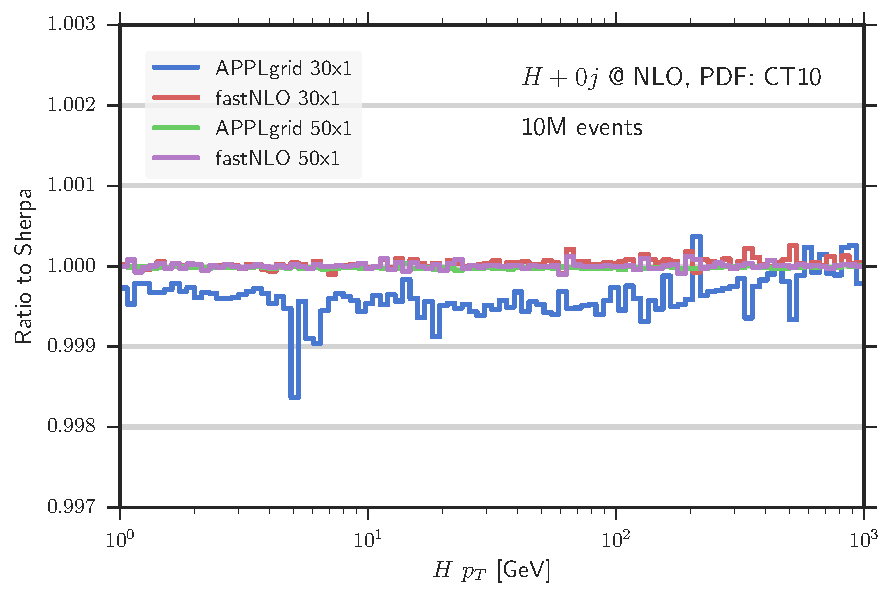
\includegraphics[width=\textwidth]{images/hnlo_hpt_50v30.pdf}
\end{subfigure}
\hfill
\begin{subfigure}[]{0.49\textwidth}
	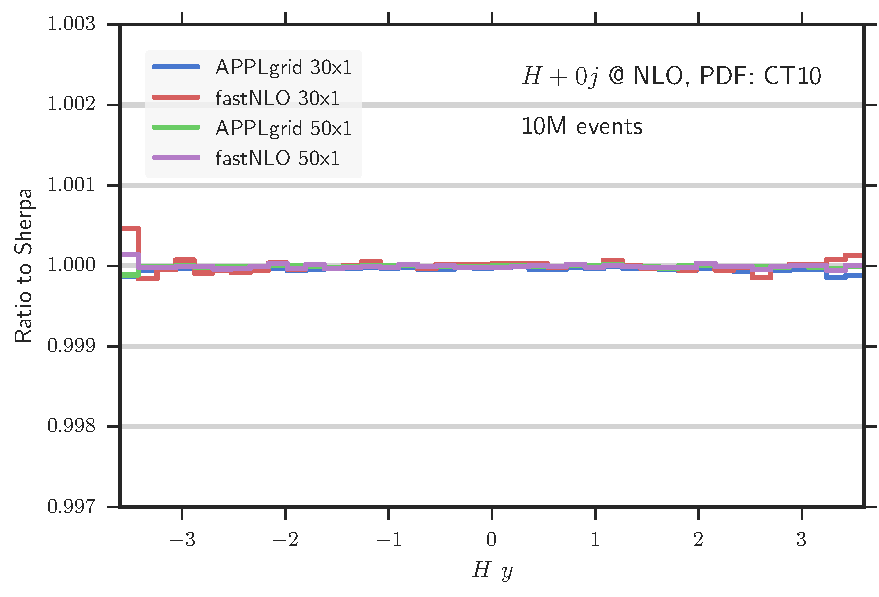
\includegraphics[width=\textwidth]{images/hnlo_hy_50v30.pdf}
\end{subfigure}

\begin{subfigure}[]{0.49\textwidth}
	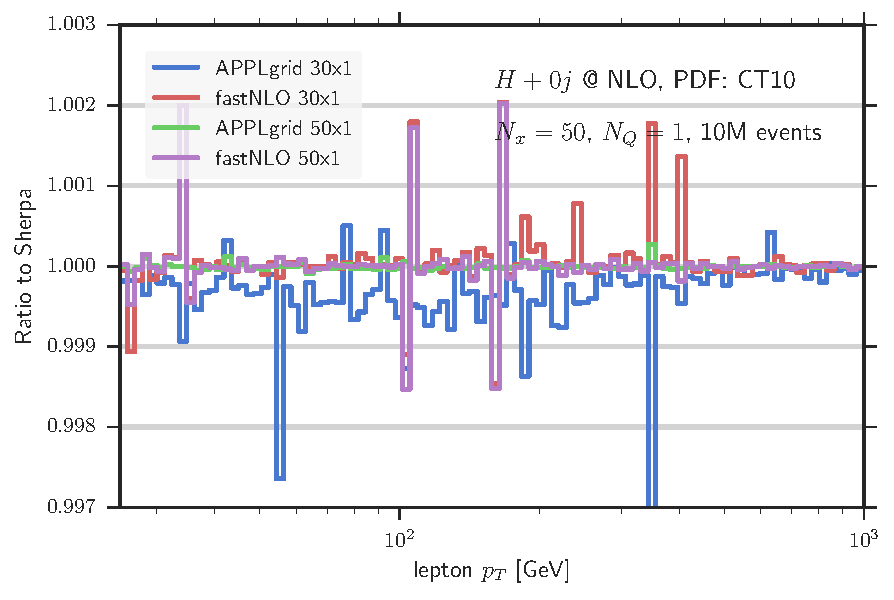
\includegraphics[width=\textwidth]{images/hnlo_lpt_50v30.pdf}
\end{subfigure}
\hfill
\begin{subfigure}[]{0.49\textwidth}
	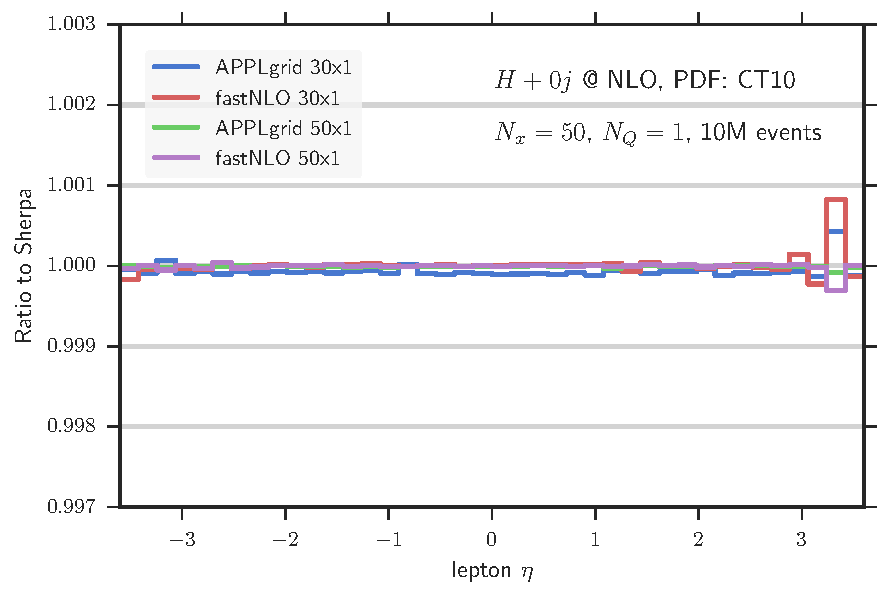
\includegraphics[width=\textwidth]{images/hnlo_leta_50v30.pdf}
\end{subfigure}
\caption{H+0j NLO}
\label{fig:hnlo_validation}
\end{sidewaysfigure}
%
\begin{sidewaysfigure}
\centering
\begin{subfigure}[]{0.49\textwidth}
	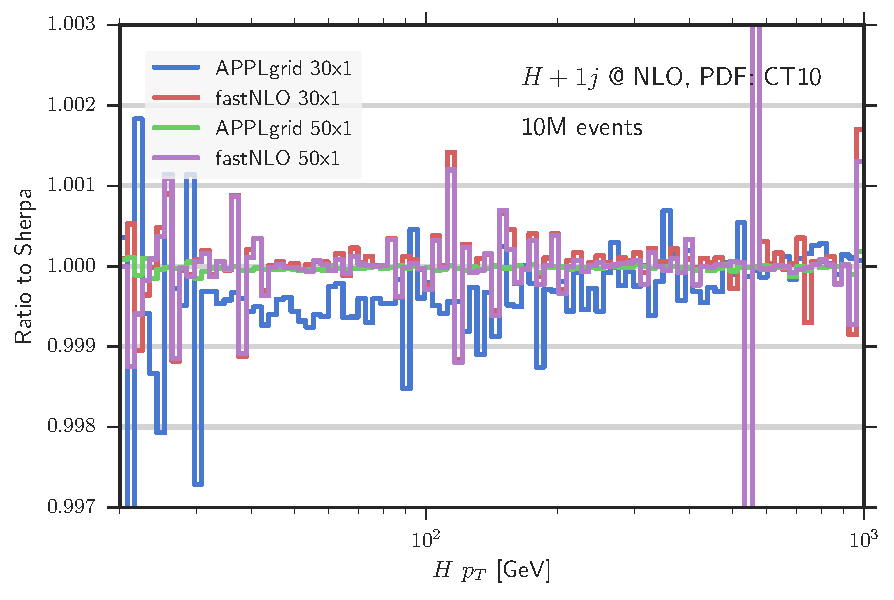
\includegraphics[width=\textwidth]{images/hjnlo_hpt_50v30.pdf}
\end{subfigure}
\hfill
\begin{subfigure}[]{0.49\textwidth}
	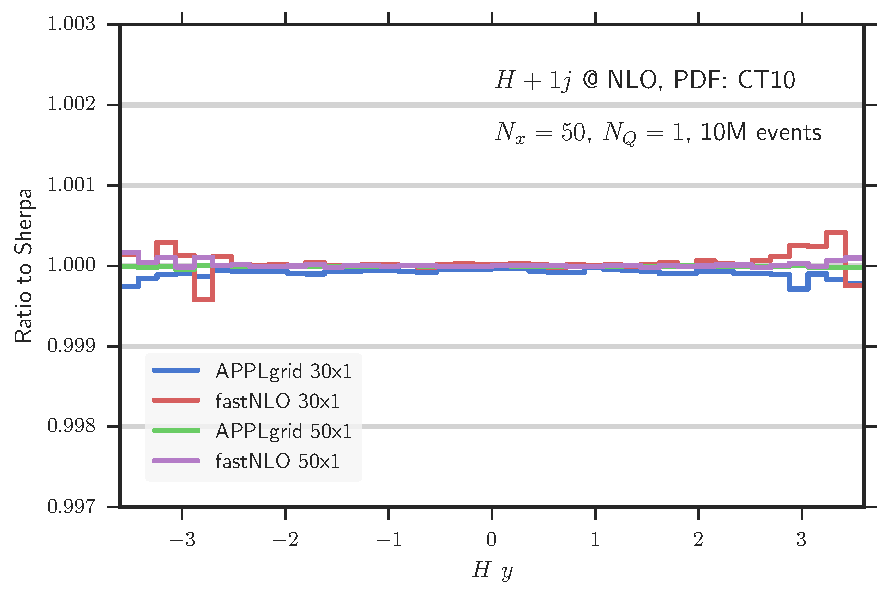
\includegraphics[width=\textwidth]{images/hjnlo_hy_50v30.pdf}
\end{subfigure}

\begin{subfigure}[]{0.49\textwidth}
	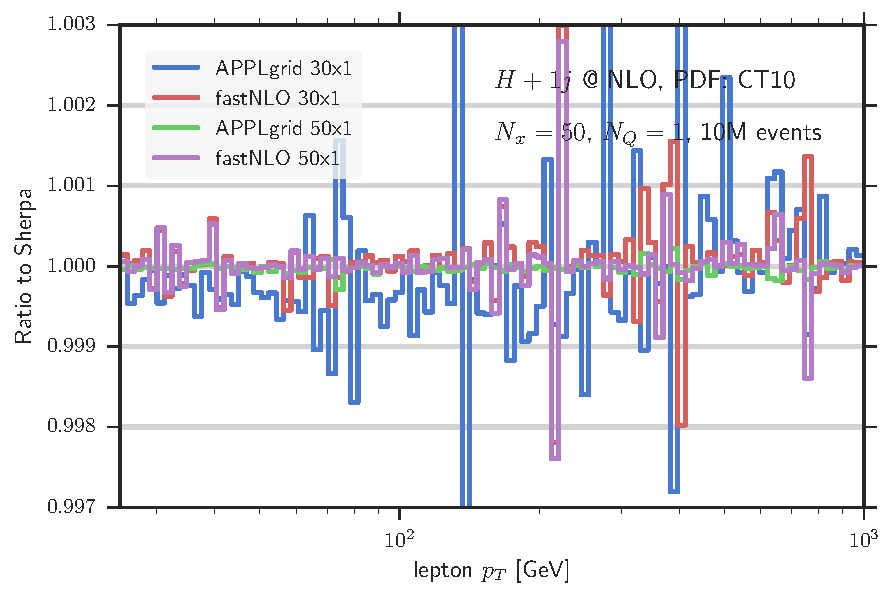
\includegraphics[width=\textwidth]{images/hjnlo_lpt_50v30.pdf}
\end{subfigure}
\hfill
\begin{subfigure}[]{0.49\textwidth}
	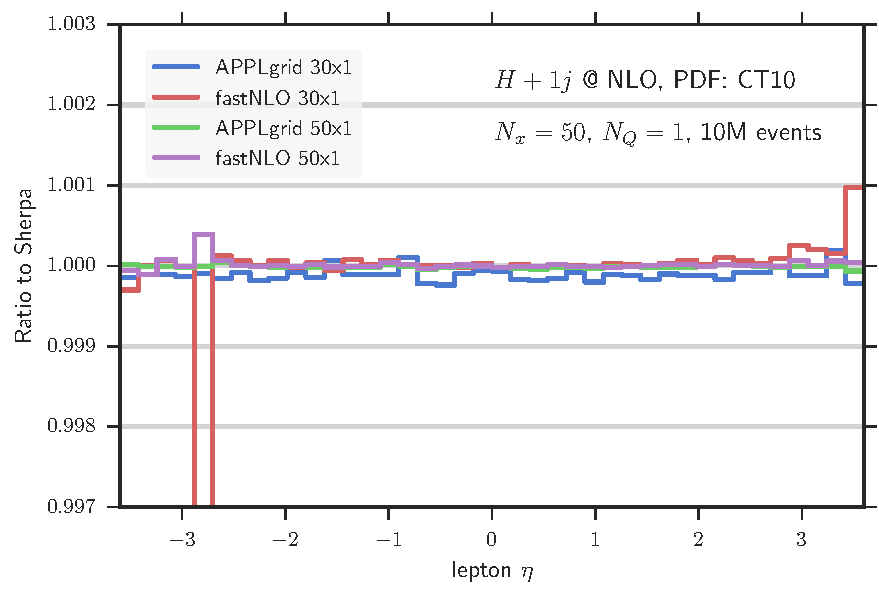
\includegraphics[width=\textwidth]{images/hjnlo_leta_50v30.pdf}
\end{subfigure}
\caption{H+1j NLO}
\label{fig:hjnlo_validation}
\end{sidewaysfigure}
%
\begin{sidewaysfigure}
\centering
\begin{subfigure}[]{0.49\textwidth}
	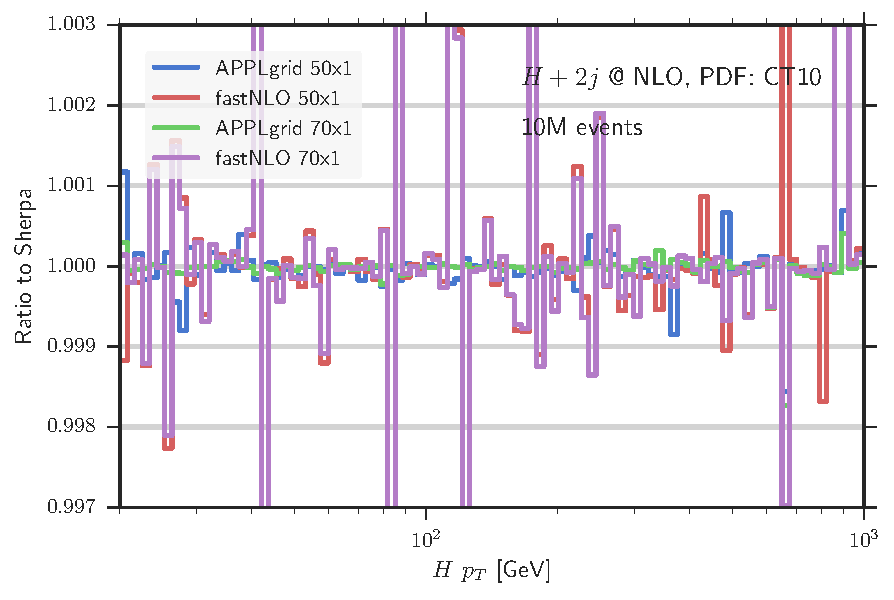
\includegraphics[width=\textwidth]{images/hjjnlo_hpt_70v50.pdf}
\end{subfigure}
\hfill
\begin{subfigure}[]{0.49\textwidth}
	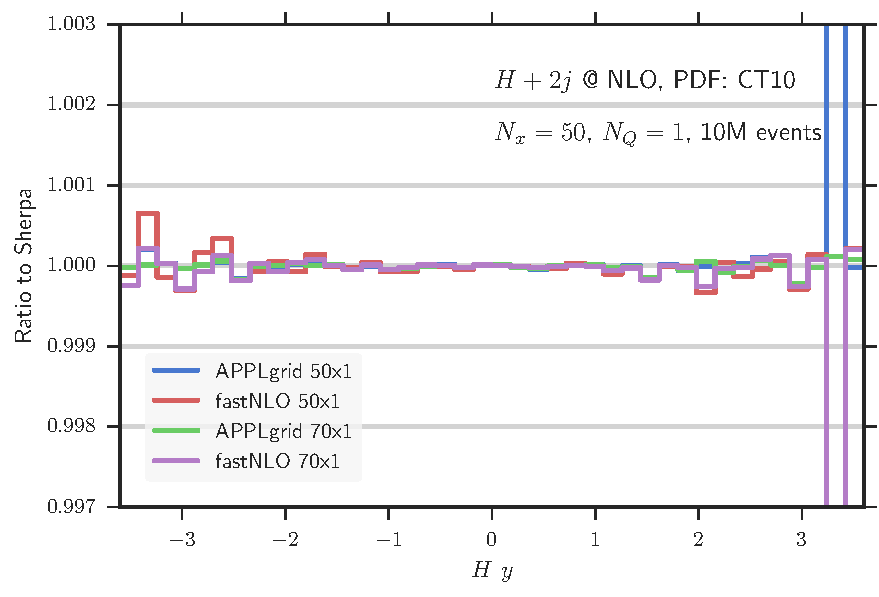
\includegraphics[width=\textwidth]{images/hjjnlo_hy_70v50.pdf}
\end{subfigure}

\begin{subfigure}[]{0.49\textwidth}
	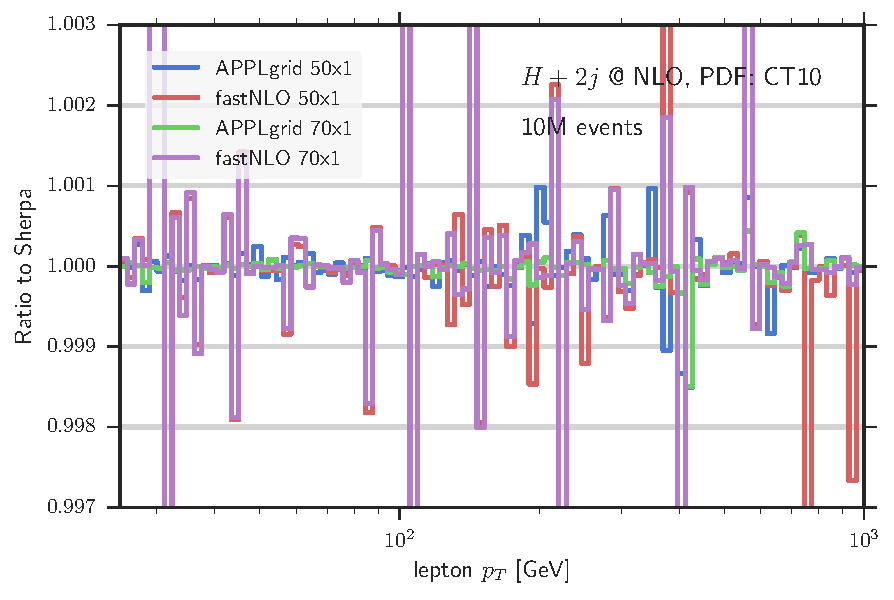
\includegraphics[width=\textwidth]{images/hjjnlo_lpt_70v50.pdf}
\end{subfigure}
\hfill
\begin{subfigure}[]{0.49\textwidth}
	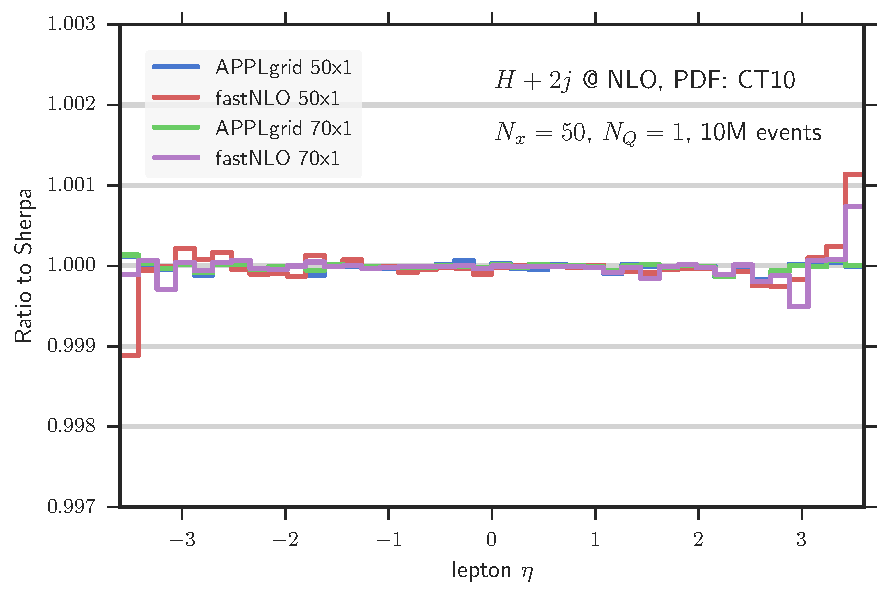
\includegraphics[width=\textwidth]{images/hjjnlo_leta_70v50.pdf}
\end{subfigure}
\caption{H+2j NLO}
\label{fig:hjjnlo_validation}
\end{sidewaysfigure}
%
\begin{figure}
	\centering
	\begin{subfigure}[]{0.49\textwidth}
		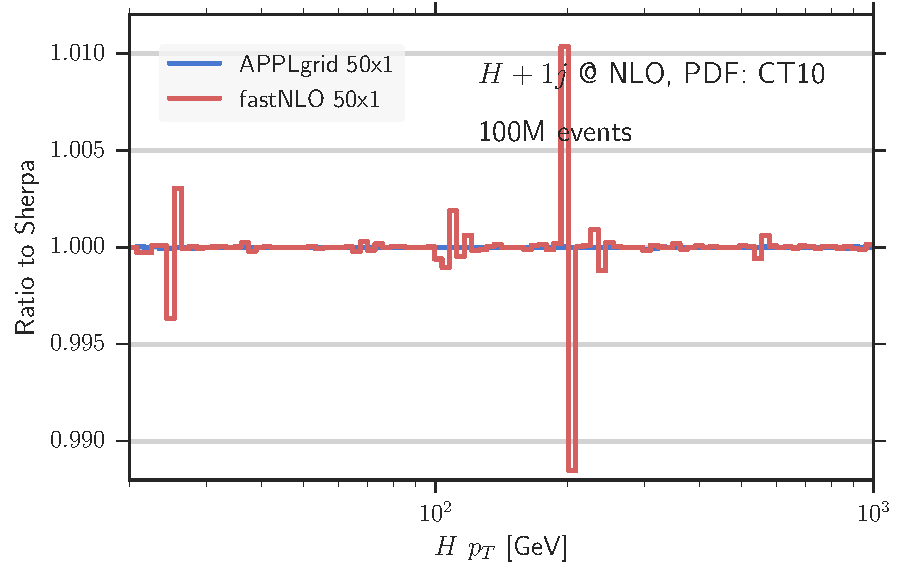
\includegraphics[width=\textwidth]{images/hjnlo_hpt_100m.pdf}
		\caption{$H + 1j$}
	\end{subfigure}
	\hfill
	\begin{subfigure}[]{0.49\textwidth}
		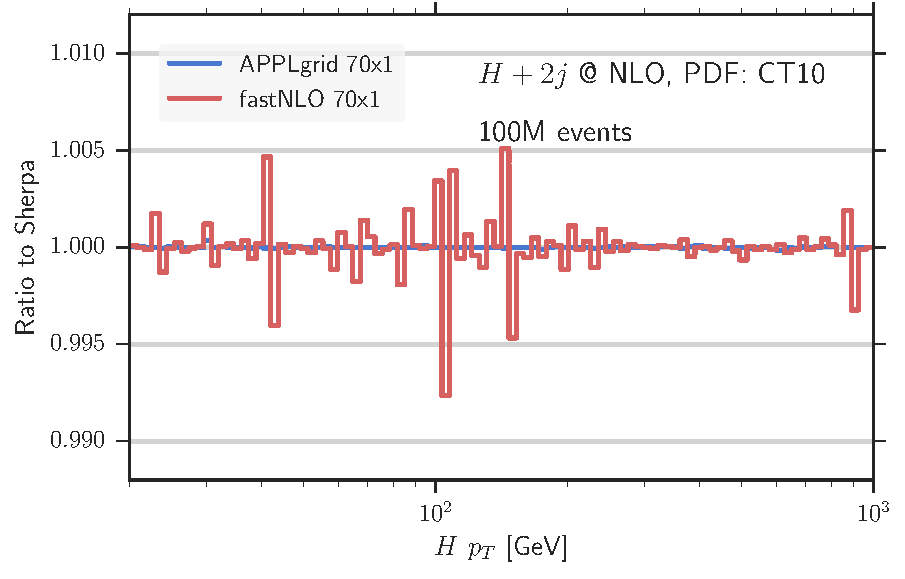
\includegraphics[width=\textwidth]{images/hjjnlo_hpt_100m.pdf}
		\caption{$H + 2j$}
	\end{subfigure}
	\caption{The effect of higher statistics on the interpolation.
				With two jets the 100 million event sample gives notably better results than the 10 million event sample in \cref{fig:hjjnlo_validation}.
				With one jet the errors are roughly the same.}
	\label{fig:hpt_100m}
\end{figure}
%
\section{Parameter variation}
\subsection{Scale factor variation}
Now that we have verified that the grids produced by \appl{} and \fnlo{} are able to reproduce the reference distributions up to the interpoation accuracy, we can take a look at the variation of the QCD parameters.
In this section we will examine the results obtained by varying the renormalization and factorization scales.
\appl{} and \fnlo{} both have methods implemented that allow to change the scales when calculating NLO cross sections.
There are different approaches to this.
The original method used by \appl{} is to apply the renormalization group equation for the renormalization scale and calculate the LO DGLAP splitting functions using \hoppet{} \cite{hoppet} to vary the factorization scale.
\fnlo{} originally did not allow the use of \hoppet{} and instead stored individual grids for each desired factorization scale.
This approach is not as flexible and leads to larger grid files but the calculation of the cross section is much faster.
However, since version 2.3 \fnlo{} can also be used in combination with \hoppet{}.
Another method, called \enquote{flexible-scale table}, is also implemented in \fnlo{}.
It stores fully scale-independent weights and allows for arbitrary and independent variation of the scale factors without the need of splitting functions.
As this feature is not yet implemented in \mcgrid{} (but will be in a future release), the first method is used in the following calculations.

The reference histograms are again generated with Sherpa using the CT10 PDF.
One central scale $\mu_R = \mu_F = m_H$ and two additional scales $2 \mu$ and $\frac{1}{2} \mu$ are used.
During the central scale run, grids for the transverse momentum of the Higgs boson are filled by \appl{} and \fnlo{} using an \mcgrid{}-enabled \rivet{} analysis.
This is done for Higgs production with zero and one jets using an event sample of 100 million events in each case.
In \cref{fig:scalesvar_hnlo_appl,fig:scalesvar_hnlo_fnlo} the reference distributions are compared to the results from \appl{} and \fnlo{} in the 0-jet case.
We observe a strong scale dependence, indicating that higher order terms entail large corrections.
This turns out to be true \cite{gfusionnnlo1,gfusionnnlo2}.
It can be seen, that the accuracy of the reproduction is very good in both cases.
The discrepancies at low $p_\perp$ in \cref{fig:scalesvar_hnlo_appl} are due to an insufficient phasespace run (the first ten million events have been used), meaning that during the fill run $x$-values emerged that were not expected by \appl{}.
The \fnlo{} grid was prepared with the same phasespace run and obviously it responds to these events in a different way resulting in a precise reproduction throughout the range of considered values.
Using a larger phasespace run, the inaccuracies with \appl{} would of course vanish.
%
\begin{figure}
	\centering
	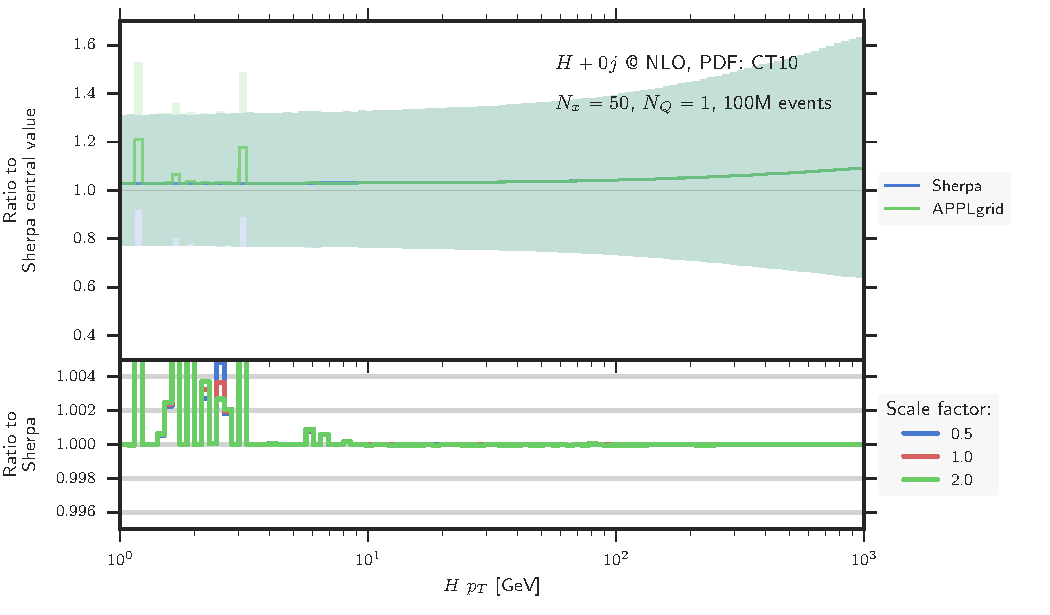
\includegraphics[width=\textwidth]{images/scalesvar_hnlo_appl.pdf}
	\caption{Scale variation appl}
	\label{fig:scalesvar_hnlo_appl}
\end{figure}
%
\begin{figure}
	\centering
	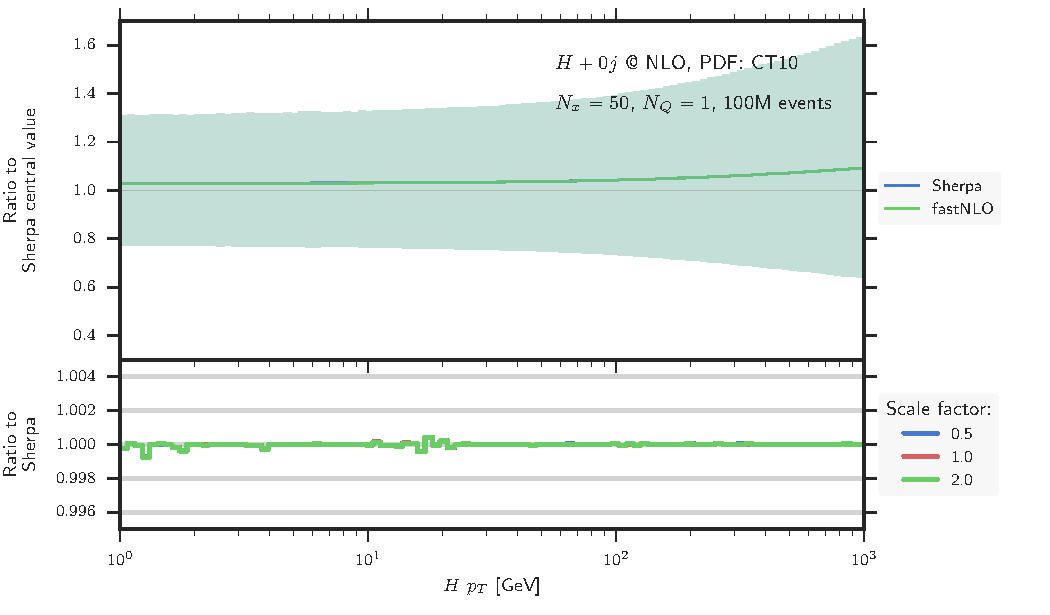
\includegraphics[width=\textwidth]{images/scalesvar_hnlo_fnlo.pdf}
	\caption{Scale variation fnlo}
	\label{fig:scalesvar_hnlo_fnlo}
\end{figure}
%

In the 1-jet case, shown in \cref{fig:scalesvar_hjnlo_appl,fig:scalesvar_hjnlo_fnlo}, the scale dependence is more complicated.
Still, \appl{} is able to reproduce all three scales at the permille level.
\fnlo{}, on the contrary, shows an unexpected behaviour.
There are systematic deviations that increase towards high transverse momenta.
As the error is definitely not caused by statistical fluctuations and because the central scale is reproduced very well, there is probably a mistake in the implementation of the evolution.
A similar behaviour can be observed with \appl{} as well, when the 2-jet case is considered.
Therefore, this does not seem to be a problem of \fnlo{} alone.
This problem is object of further investigations.
%
\begin{figure}
	\centering
	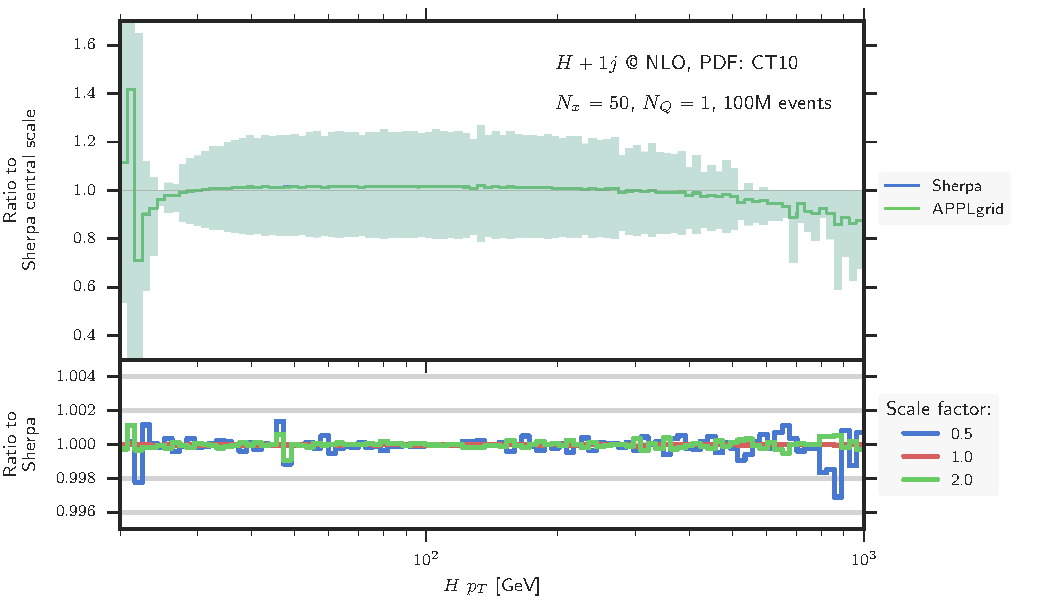
\includegraphics[width=\textwidth]{images/scalesvar_hjnlo_appl.pdf}
	\caption{Scale variation appl}
	\label{fig:scalesvar_hjnlo_appl}
\end{figure}
%
\begin{figure}
	\centering
	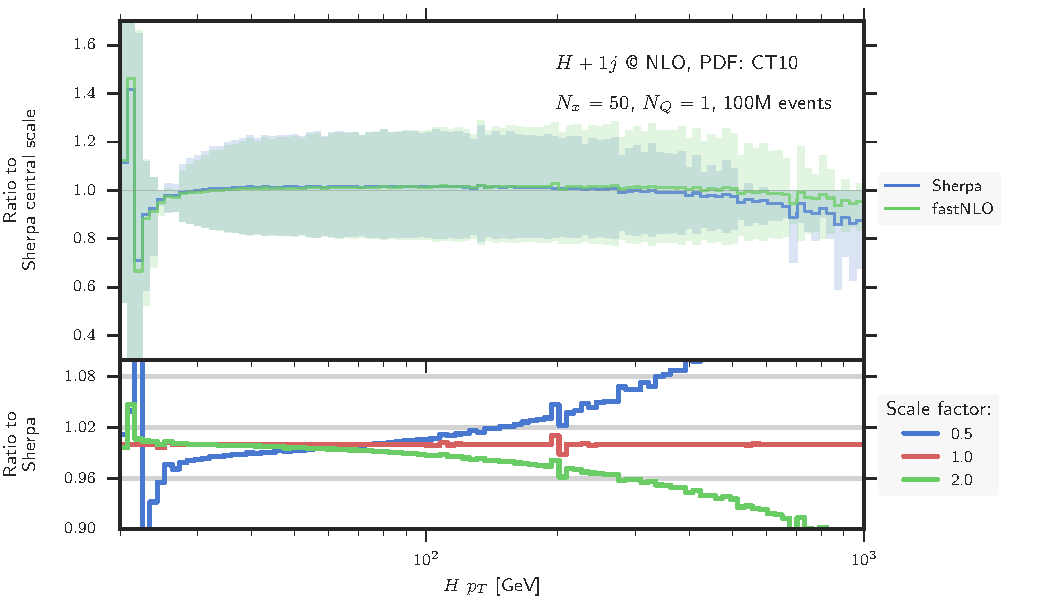
\includegraphics[width=\textwidth]{images/scalesvar_hjnlo_fnlo.pdf}
	\caption{Scale variation fnlo}
	\label{fig:scalesvar_hjnlo_fnlo}
\end{figure}
%
\subsection{Reweighting to a different PDF}
In addition to the variation of the scale factors, it is possible to change the PDF as well.
As an example, the transverse momentum of the Higgs boson is considered again.
Grids that have been filled with the CT10 PDF are convoluted with the central value of the NNPDF3.0 set \textit{a posteriori}.
They are compared to the reference distribution, that has been produced by \sherpa{} using NNPDF3.0 explicitly, at three different scales.
The results are shown in \cref{fig:pdfvar_hnlo_appl,fig:pdfvar_hnlo_fnlo} for \appl{} and \fnlo{}, respectively.
Again, we observe a very good reproduction.
The magnitude of the errors is similar to the results of the previous section (cf. \cref{fig:scalesvar_hnlo_appl,fig:scalesvar_hnlo_fnlo}).
As has already been explained above, the discrepancies in the \appl{} plot at low $p_\perp$ originate from an insufficient phasespace run that did not cover the whole $x$-range.
They do not indicate any problems with the interpolation (which is proven by the \fnlo{} result in \cref{fig:pdfvar_hnlo_fnlo}) and are fixable.
%
\begin{figure}
	\centering
	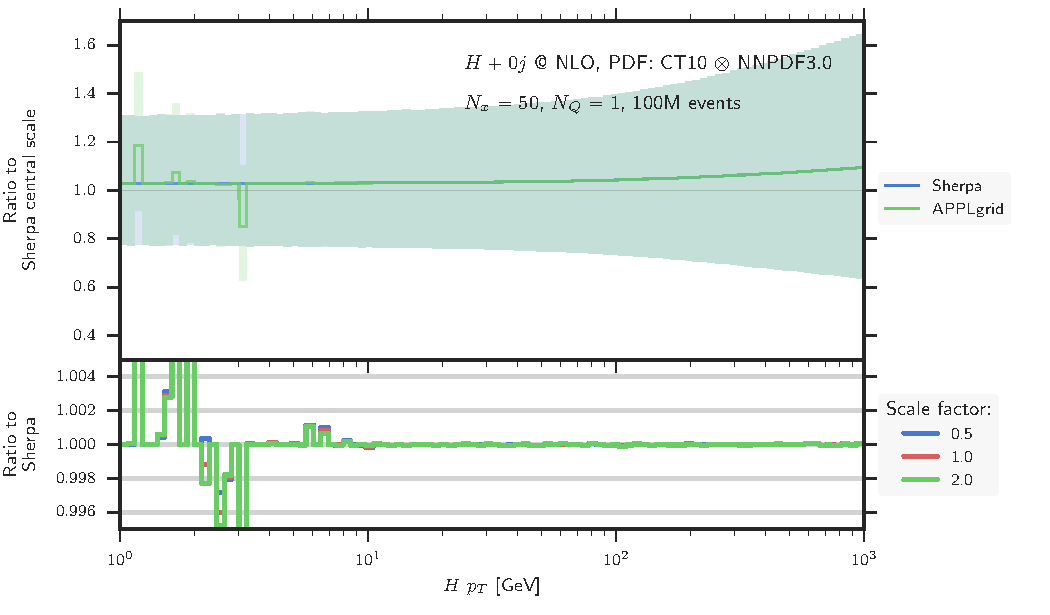
\includegraphics[width=\textwidth]{images/pdfvar_hnlo_appl.pdf}
	\caption{PDF variation appl}
	\label{fig:pdfvar_hnlo_appl}
\end{figure}
%
\begin{figure}
	\centering
	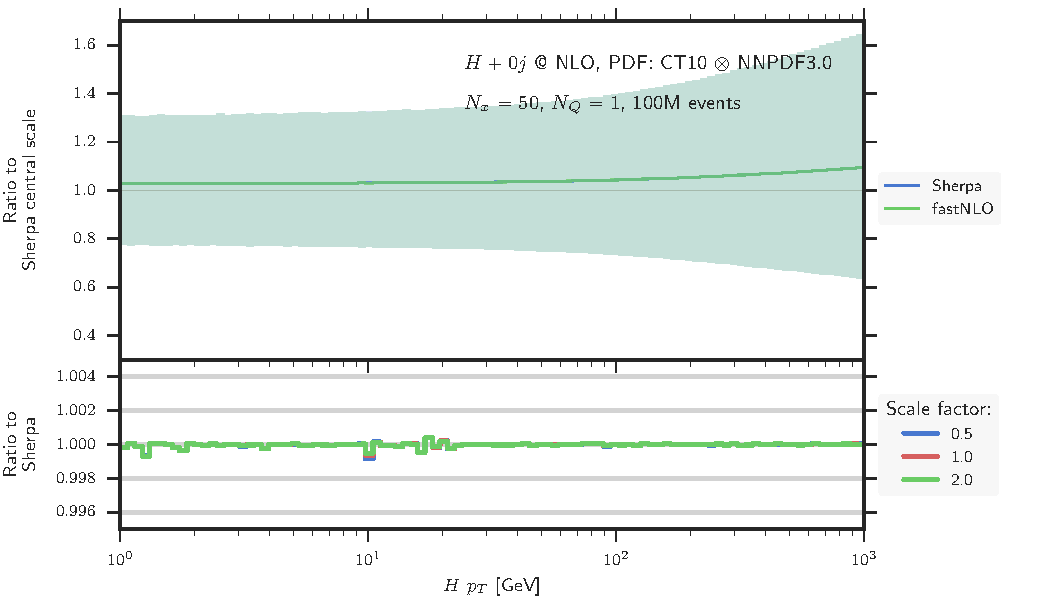
\includegraphics[width=\textwidth]{images/pdfvar_hnlo_fnlo.pdf}
	\caption{PDF variation fnlo}
	\label{fig:pdfvar_hnlo_fnlo}
\end{figure}
%

% !TeX encoding=unicode
% !TeX spellcheck = en-US

\chapter{Application examples}
\label{ch:examples}
This chapter presents two examples of application for interpolation grids.
They demonstrate how they extend the number of possible calculations and allow a level of detail in the study of uncertainties that would be very expensive otherwise.
%
\section{PDF uncertainty in cross section calculations}
The application of the interpolation method is sensible every time a calculation has to be repeated plenty of times.
This situation is given for instance, when the uncertainty from a PDF set is meant to be included in a cross section calculation.
Modern PDF sets contain a large number of different samples that can be used to derive the inherent uncertainty.
Having verified that the interpolation grids allow for PDF reweighting in the previous chapter, it is now justified to use them to compute the PDF uncertainty.
Here we consider the NNPDF 3.0 NLO set \cite{nnpdf30}, which consists of \num{101} samples each for \num{5} different values of $\alpha_s$ between \num{0.115} and \num{0.121}.
The grid that has been filled with 100 million events using the central value of the CT10 set is used to calculate a total of 505 replicas for the Higgs $p_\perp$ in \cref{fig:nnpdf_band}.
The similarity between the \appl{} and \fnlo{} plots confirms the correctness of the calculation, as inaccuracies would propagate quite differently in the two implementations.
Once again we see the effects of an insufficient phase space run that have already appeared in \cref{fig:scalesvar_hnlo_appl,fig:pdfvar_hnlo_appl}.
Another thing to observe is that the PDF uncertainty is significantly smaller than the scale uncertainty, even when combined with the error on $\alpha_s$.
The ratio between them is roughly $\frac{1}{6}$.
%
\begin{figure}
	\centering
	\begin{subfigure}[]{0.49\textwidth}
		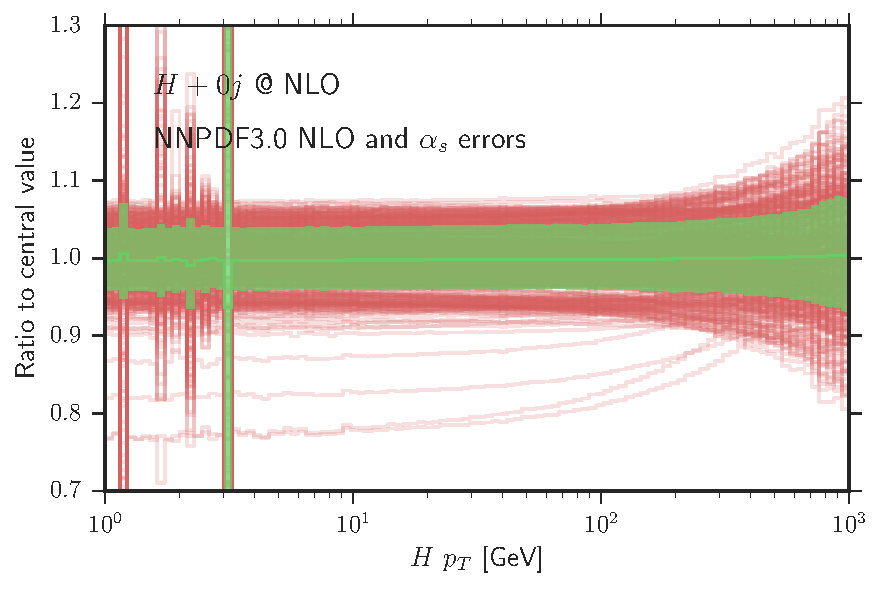
\includegraphics[width=\textwidth]{images/nnpdf_band_appl.pdf}
		\caption{\appl{}}
	\end{subfigure}
	\hfill
	\begin{subfigure}[]{0.49\textwidth}
		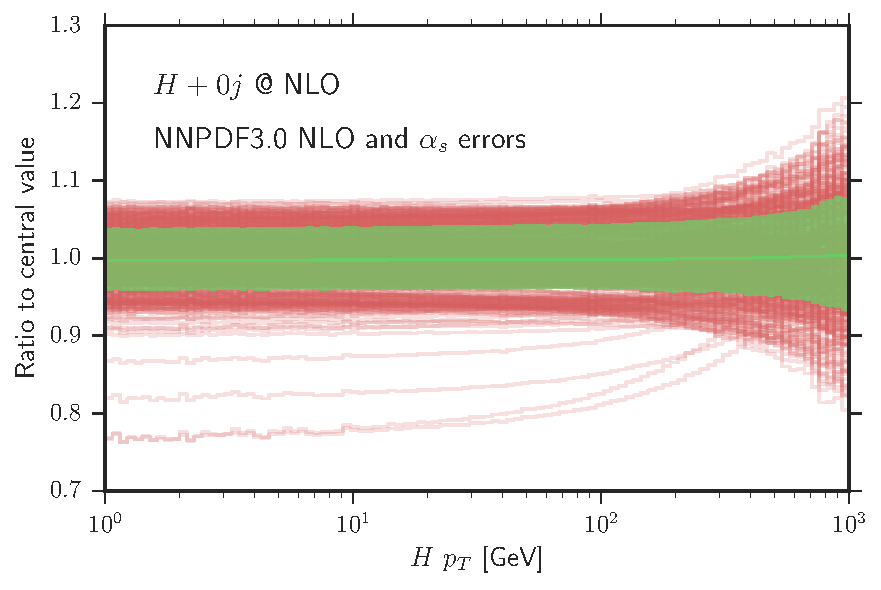
\includegraphics[width=\textwidth]{images/nnpdf_band_fnlo.pdf}
		\caption{\fnlo{}}
	\end{subfigure}
	\caption{Application example of the interpolation method.
				The figure shows the distribution of replicas from the NNPDF3.0 NLO set including the error on $\alpha_s$ for the $p_\perp$ of the Higgs boson in gluon fusion.
				The green area highlights the 1-$\sigma$ confidence interval.}
	\label{fig:nnpdf_band}
\end{figure}
%
\section{Detailed scale dependence of the cross section}
When one wishes to estimate the uncertainty of a fixed order calculation, a common method is to vary the renormalization and factorization scales simultaneously or independently by some factor, usually a factor of 2.
This way one hopes to get a reasonable estimate of the corrections due to higher order terms.
Typically, only the boundary values are calculated because of limited resources.
However, using interpolation grids, any combination of scale factors can be evaluated very fast.
To demonstrate this, \cref{fig:3dscale} shows the total cross section of inclusive Higgs production through gluon fusion for different combinations of scale factors, calculated using a \fnlo{} grid.
Both the renormalization scale and the factorization scale are independently varied by 13 factors between $\frac{1}{4}$ and \num{4} resulting in a total number of 169 calculations of the cross section.
We see that the dependence on the factorization scale is low whereas we observe a strong dependence on the renormalization scale.
%
\begin{figure}
	\centering
	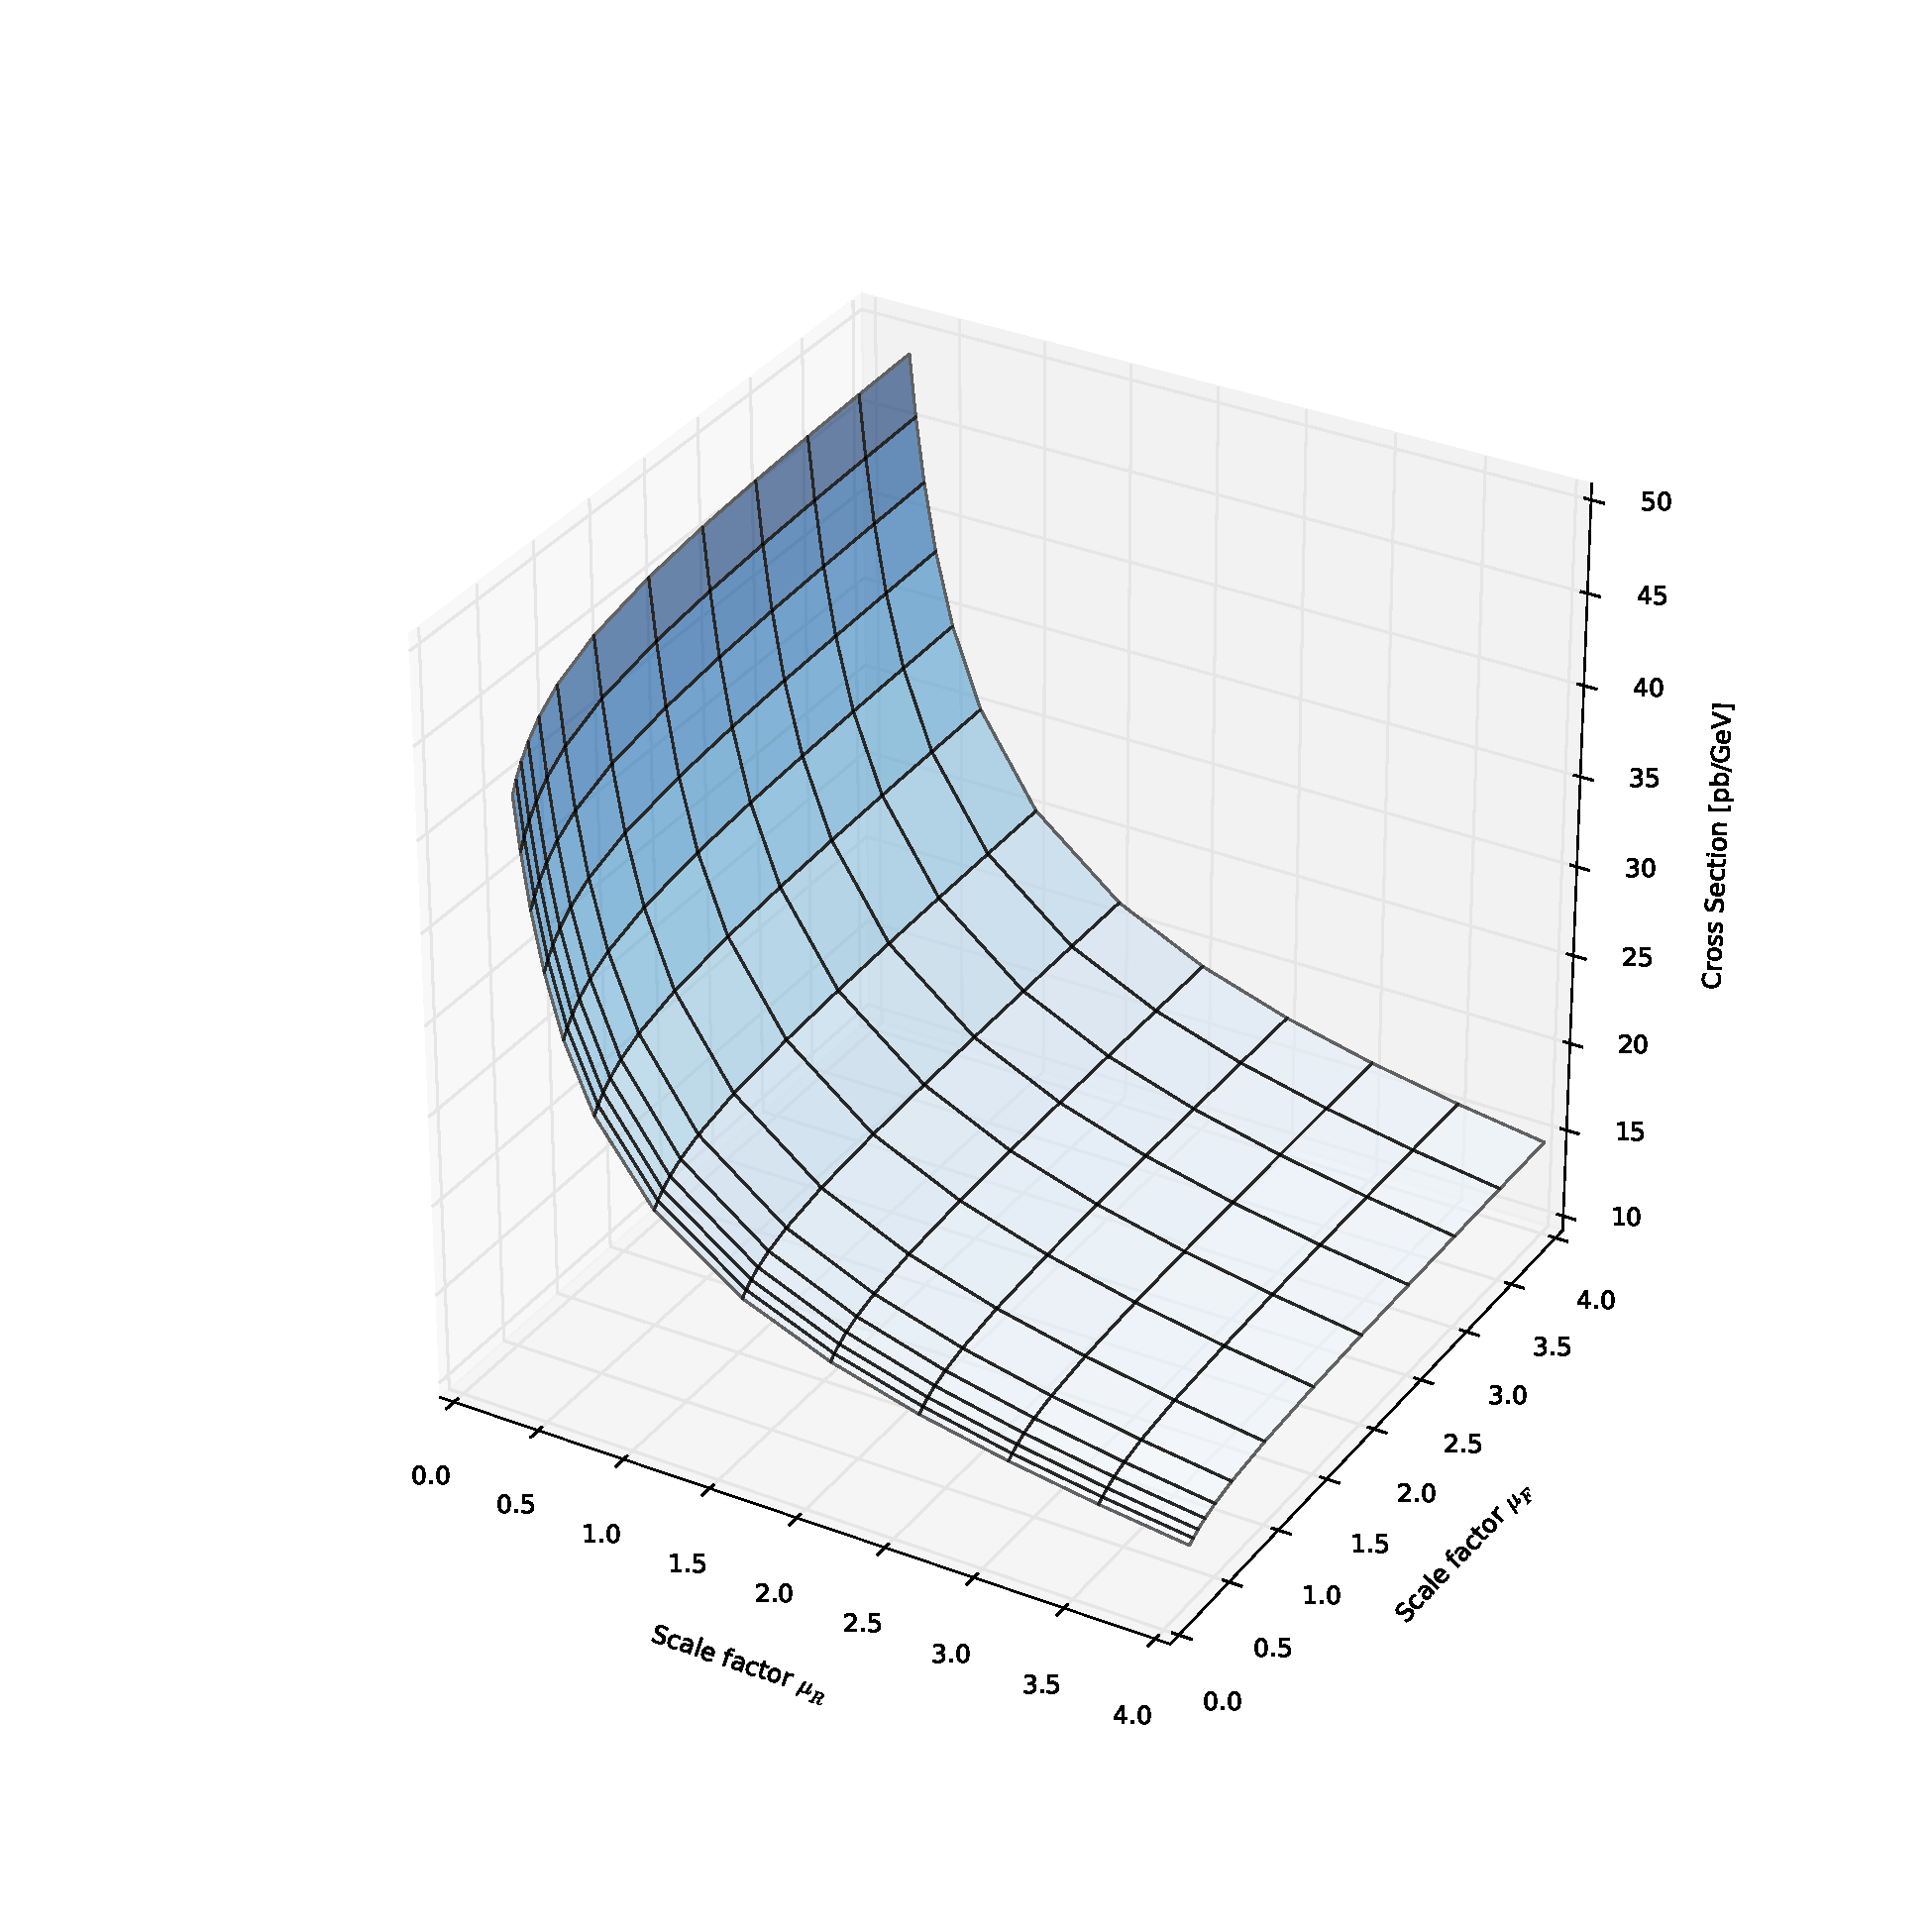
\includegraphics[width=0.8\textwidth]{images/3dscale.pdf}
	\caption{Application example of the interpolation method}
	\label{fig:3dscale}
\end{figure}
%

Calculations such as this one and the example illustrated before would be extremely costly if done explicitly.
If they are time-critical, explicit calculations become impossible.
Interpolation tools offer much more flexibility in these cases.
Especially the estimation of uncertainties can be much more differentiated.

% !TeX encoding=unicode
% !TeX spellcheck = de-DE

\chapter{Conclusion}
In this thesis, an interpolation method has been used to accelerate the variation of parameters in a fixed order NLO calculation.
\mcgrid{} has been used to interface two different tools, \appl{} and \fnlo{}, which have been used to fill interpolation grids with the correct information.
This has been performed explicitly for the example of Higgs boson production at the LHC.
It could be verified that the applied method is able to achieve sub-percent accuracy in the reproduction of different observables.
The possibility of \textit{a posteriori} variation of the renormalization and factorization scales has been demonstrated.
It shows no significant decrease in accuracy when no additional hard jets are considered but problems in the reproduction emerged in the cases of one and two additional jets (cf. \cref{sec:scalesvar}).
They seem to be caused by the technique that is used to variate the scales and not by errors in the interpolation method itself.
Future investigations will isolate the cause of the problem and deduce what is needed to fix it.
Changing the PDF during the reevaluation of the cross section, however, has caused no further problems and has provided reproduction accuracy at permille level.

Two examples have been demonstrated that give an impression of possible applications.
Global PDF fits benefit from the possibilty of evaluating a large number of PDFs in cross section calculations.
Without tools like \appl{} and \fnlo{}, many processes could not be included in fits beyond LO.
In addition to that, the interpolation tools simplify the treatment of uncertainties in theoretical predictions based on Monte Carlo event generators.

Further studies concerning the use of \mcgrid{} in the Higgs production process could include dynamically allocated scales.
This case adds further complexity to the interpolation grids as the dependence on the scales has to be interpolated as well.
It could not be validated yet.
In a next step the support of the fixed order expansion of \mcatnlo{}, which is introduced in version 2.0 of \mcgrid{}, needs to be verified as well.
That would pave the way for a complete inclusion of multijet merged calculations.
It is a desirable goal, because merged calculations are very complex and time consuming and therefore are very well suited for a method that allows faster computation.
%... 
%
%Version 2.0 of \mcgrid{} will allow the creation of grids for calculations matching NLO QCD computations and parton showers using \mcatnlo{}.
%This has not been verified yet for Higgs production.
%However, as has been seen in section \textcolor{red}{???} the \mcatnlo{} approach allows for a more accurate description of soft and collinear emissions than fixed order NLO calculations.
%Therefore ...

In \cref{sec:xtransform} we examined how \appl{} and \fnlo{} parametrize the $x$\-/distribution to provide a better coverage of the data on a grid with equal-sized bins.
Which transformation should be used depends on the considered observable.
To achieve the best possible performance, one would have to check the actual $x$-distribution in each case.
The provided transformations are obviously a compromise to cover the needs of a large number of processes.
The drawback of this approach is that for some observables one needs unnecessary large grids to reliably reproduce them.
There is, however, an alternative way: When performing the phasespace run prior to the fill run one could, instead of only determining the limit values of $x$ and $Q^2$, sample the whole distribution.
By the use of numerical inversion, the data could then be used to provide a transformation that represents the actual distribution of $x$ or $Q^2$ in the process.
Thus, the bins of the grid would be filled ideally and a smaller grid would suffice to reproduce the desired observable.
This would improve the overall performance of the software, as a smaller grid means less computation time and less memory consumption.


% !TeX encoding=unicode
% !TeX spellcheck = de-DE

% change parskip
\setlength\parindent{0pt} 
\setlength\parskip{\medskipamount}

% chapter without heading and without number
% \addchap*{Acknowledgements}
\addchap*{Acknowledgements}
%
I'd like to thank my supervisor Steffen Schumann for giving me the chance to be a part of this interesting project as well as for his encouragement and for always trying his best in answering my various questions.
Furthermore I'm very grateful for the support from Enrico Bothmann, who helped me with the technical aspects of my study and never hesitated to provide me the required information or to take a deeper look at my issues.
Without his help, I would not have come as far as I did during the time of my thesis.

\cleardoublepage


%%% -- end of main content

%%% -- list of figures and tables --
%\cleardoublepage\IfDefined{phantomsection}{\phantomsection}\label{sec:lof}
%\listoffigures
%\cleardoublepage\IfDefined{phantomsection}{\phantomsection}\label{sec:lot}
%\listoftables
%
%%% -- List of Listings --
%% _Remove_ if no listing with caption is defined
%\IfDefined{lstlistoflistings}{\cleardoublepage\lstlistoflistings}
%
%% --- Appendix --- --- --- --- --- --- ---
%\cleardoublepage
%\appendix
%% Add `Appendix` to TOC
%\addcontentsline{toc}{part}{\appendixname}
%% must be _input_, otherwise the TOC entry is at the wrong place
%% !TeX encoding=unicode
% !TeX spellcheck = de-DE

%
% add files for appendix chapter here
%\chapter{Erster Anhang}



% -- bibliography --
% (must be placed _after_ appendix)
\IfPackageLoaded{biblatex}{
  \cleardoublepage
  \IfDefined{phantomsection}{\phantomsection}\label{sec:bibliography}
  \printbibliography[%
    heading=bibintoc, % (bibintoc, bibnumbered)
  ]	
}% end of bibliography

%% -- Index --
% _Remove_ Index unless you really want to invest a large amount
% of time and effort to create a good index!
\IfDefined{printindex}{%
  \cleardoublepage\IfDefined{phantomsection}{\phantomsection}\label{sec:index}%
  \printindex%
}% end of index

% -- declaration --
% (only in bachelor/master thesis)
% !TeX encoding=unicode
% !TeX spellcheck = de-DE

\Declaration


% add todo list (remove for final document!)
%\IfPackageLoaded{todonotes}{
  \clearpage
  \IfPackageLoaded{hyperref}{\phantomsection}
  \todototoc   % add to toc 
  \listoftodos % print to document
}


%%% document END %%%%%%%%%%%%%%%%%%%%%%%%%%%%%%%%%%%%%%%%%%%%%%%%%%%%%%%%%%%
\end{document}
%%%%%%%%%%%%%%%%%%%%%%%%%%%%%%%%%%%%%%%%%%%%%%%%%%%%%%%%%%%%%%%%%%%%%%%%%%%%
